\documentclass[twoside]{book}

% Packages required by doxygen
\usepackage{calc}
\usepackage{doxygen}
\usepackage{graphicx}
\usepackage[utf8]{inputenc}
\usepackage{makeidx}
\usepackage{multicol}
\usepackage{multirow}
\usepackage{textcomp}
\usepackage[table]{xcolor}

% NLS support packages
\usepackage[T2A]{fontenc}
\usepackage[russian]{babel}

% Font selection
\usepackage[T1]{fontenc}
\usepackage{mathptmx}
\usepackage[scaled=.90]{helvet}
\usepackage{courier}
\usepackage{amssymb}
\usepackage{sectsty}
\renewcommand{\familydefault}{\sfdefault}
\allsectionsfont{%
  \fontseries{bc}\selectfont%
  \color{darkgray}%
}
\renewcommand{\DoxyLabelFont}{%
  \fontseries{bc}\selectfont%
  \color{darkgray}%
}

% Page & text layout
\usepackage{geometry}
\geometry{%
  a4paper,%
  top=2.5cm,%
  bottom=2.5cm,%
  left=2.5cm,%
  right=2.5cm%
}
\tolerance=750
\hfuzz=15pt
\hbadness=750
\setlength{\emergencystretch}{15pt}
\setlength{\parindent}{0cm}
\setlength{\parskip}{0.2cm}
\makeatletter
\renewcommand{\paragraph}{%
  \@startsection{paragraph}{4}{0ex}{-1.0ex}{1.0ex}{%
    \normalfont\normalsize\bfseries\SS@parafont%
  }%
}
\renewcommand{\subparagraph}{%
  \@startsection{subparagraph}{5}{0ex}{-1.0ex}{1.0ex}{%
    \normalfont\normalsize\bfseries\SS@subparafont%
  }%
}
\makeatother

% Headers & footers
\usepackage{fancyhdr}
\pagestyle{fancyplain}
\fancyhead[LE]{\fancyplain{}{\bfseries\thepage}}
\fancyhead[CE]{\fancyplain{}{}}
\fancyhead[RE]{\fancyplain{}{\bfseries\leftmark}}
\fancyhead[LO]{\fancyplain{}{\bfseries\rightmark}}
\fancyhead[CO]{\fancyplain{}{}}
\fancyhead[RO]{\fancyplain{}{\bfseries\thepage}}
\fancyfoot[LE]{\fancyplain{}{}}
\fancyfoot[CE]{\fancyplain{}{}}
\fancyfoot[RE]{\fancyplain{}{\bfseries\scriptsize Документация по graph\-Editor. Последние изменения\-: Пн 4 Янв 2021 05\-:02\-:15. Создано системой Doxygen }}
\fancyfoot[LO]{\fancyplain{}{\bfseries\scriptsize Документация по graph\-Editor. Последние изменения\-: Пн 4 Янв 2021 05\-:02\-:15. Создано системой Doxygen }}
\fancyfoot[CO]{\fancyplain{}{}}
\fancyfoot[RO]{\fancyplain{}{}}
\renewcommand{\footrulewidth}{0.4pt}
\renewcommand{\chaptermark}[1]{%
  \markboth{#1}{}%
}
\renewcommand{\sectionmark}[1]{%
  \markright{\thesection\ #1}%
}

% Indices & bibliography
\usepackage{natbib}
\usepackage[titles]{tocloft}
\setcounter{tocdepth}{3}
\setcounter{secnumdepth}{5}
\makeindex

% Hyperlinks (required, but should be loaded last)
\usepackage{ifpdf}
\ifpdf
  \usepackage[pdftex,pagebackref=true]{hyperref}
\else
  \usepackage[ps2pdf,pagebackref=true]{hyperref}
\fi
\hypersetup{%
  colorlinks=true,%
  linkcolor=blue,%
  citecolor=blue,%
  unicode%
}

% Custom commands
\newcommand{\clearemptydoublepage}{%
  \newpage{\pagestyle{empty}\cleardoublepage}%
}


%===== C O N T E N T S =====

\begin{document}

% Titlepage & ToC
\hypersetup{pageanchor=false}
\pagenumbering{roman}
\begin{titlepage}
\vspace*{7cm}
\begin{center}%
{\Large graph\-Editor }\\
\vspace*{1cm}
{\large Создано системой Doxygen 1.8.6}\\
\vspace*{0.5cm}
{\small Пн 4 Янв 2021 05:02:15}\\
\end{center}
\end{titlepage}
\clearemptydoublepage
\tableofcontents
\clearemptydoublepage
\pagenumbering{arabic}
\hypersetup{pageanchor=true}

%--- Begin generated contents ---
\chapter{Иерархический список классов}
\section{Иерархия классов}
Иерархия классов.\begin{DoxyCompactList}
\item \contentsline{section}{Controller}{\pageref{class_controller}}{}
\begin{DoxyCompactList}
\item \contentsline{section}{Create\-Controller}{\pageref{class_create_controller}}{}
\item \contentsline{section}{Delete\-Controller}{\pageref{class_delete_controller}}{}
\item \contentsline{section}{Load\-Controller}{\pageref{class_load_controller}}{}
\item \contentsline{section}{Multyline\-Controller}{\pageref{class_multyline_controller}}{}
\begin{DoxyCompactList}
\item \contentsline{section}{Quadrangle\-Controller}{\pageref{class_quadrangle_controller}}{}
\begin{DoxyCompactList}
\item \contentsline{section}{Parallelogram\-Controller}{\pageref{class_parallelogram_controller}}{}
\item \contentsline{section}{Rectangle\-Controller}{\pageref{class_rectangle_controller}}{}
\item \contentsline{section}{Rhombous\-Controller}{\pageref{class_rhombous_controller}}{}
\item \contentsline{section}{Square\-Controller}{\pageref{class_square_controller}}{}
\end{DoxyCompactList}
\item \contentsline{section}{Section\-Controller}{\pageref{class_section_controller}}{}
\item \contentsline{section}{Triangle\-Controller}{\pageref{class_triangle_controller}}{}
\begin{DoxyCompactList}
\item \contentsline{section}{Equilateral\-Triangle\-Controller}{\pageref{class_equilateral_triangle_controller}}{}
\item \contentsline{section}{Isosceles\-Triangle\-Controller}{\pageref{class_isosceles_triangle_controller}}{}
\item \contentsline{section}{Versatile\-Triangle\-Controller}{\pageref{class_versatile_triangle_controller}}{}
\end{DoxyCompactList}
\end{DoxyCompactList}
\item \contentsline{section}{Save\-Controller}{\pageref{class_save_controller}}{}
\end{DoxyCompactList}
\item \contentsline{section}{Main\-Controller}{\pageref{class_main_controller}}{}
\item \contentsline{section}{Model}{\pageref{class_model}}{}
\item \contentsline{section}{Multyline}{\pageref{class_multyline}}{}
\begin{DoxyCompactList}
\item \contentsline{section}{Quadrangle}{\pageref{class_quadrangle}}{}
\begin{DoxyCompactList}
\item \contentsline{section}{Parallelogram}{\pageref{class_parallelogram}}{}
\item \contentsline{section}{Rectangle}{\pageref{class_rectangle}}{}
\item \contentsline{section}{Rhombous}{\pageref{class_rhombous}}{}
\item \contentsline{section}{Square}{\pageref{class_square}}{}
\item \contentsline{section}{Versatile\-Quadrangle}{\pageref{class_versatile_quadrangle}}{}
\end{DoxyCompactList}
\item \contentsline{section}{Section}{\pageref{class_section}}{}
\item \contentsline{section}{Triangle}{\pageref{class_triangle}}{}
\begin{DoxyCompactList}
\item \contentsline{section}{Equilateral\-Triangle}{\pageref{class_equilateral_triangle}}{}
\item \contentsline{section}{Isosceles\-Triangle}{\pageref{class_isosceles_triangle}}{}
\item \contentsline{section}{Versatile\-Triangle}{\pageref{class_versatile_triangle}}{}
\end{DoxyCompactList}
\end{DoxyCompactList}
\item \contentsline{section}{Point}{\pageref{class_point}}{}
\item \contentsline{section}{View}{\pageref{class_view}}{}
\item \contentsline{section}{View\-Object}{\pageref{class_view_object}}{}
\begin{DoxyCompactList}
\item \contentsline{section}{Button}{\pageref{class_button}}{}
\item \contentsline{section}{Canvas}{\pageref{class_canvas}}{}
\end{DoxyCompactList}
\end{DoxyCompactList}

\chapter{Алфавитный указатель классов}
\section{Классы}
Классы с их кратким описанием.\begin{DoxyCompactList}
\item\contentsline{section}{\hyperlink{class_button}{Button} }{\pageref{class_button}}{}
\item\contentsline{section}{\hyperlink{class_canvas}{Canvas} }{\pageref{class_canvas}}{}
\item\contentsline{section}{\hyperlink{class_controller}{Controller} }{\pageref{class_controller}}{}
\item\contentsline{section}{\hyperlink{class_create_controller}{Create\-Controller} }{\pageref{class_create_controller}}{}
\item\contentsline{section}{\hyperlink{class_delete_controller}{Delete\-Controller} }{\pageref{class_delete_controller}}{}
\item\contentsline{section}{\hyperlink{class_equilateral_triangle}{Equilateral\-Triangle} }{\pageref{class_equilateral_triangle}}{}
\item\contentsline{section}{\hyperlink{class_equilateral_triangle_controller}{Equilateral\-Triangle\-Controller} }{\pageref{class_equilateral_triangle_controller}}{}
\item\contentsline{section}{\hyperlink{class_isosceles_triangle}{Isosceles\-Triangle} }{\pageref{class_isosceles_triangle}}{}
\item\contentsline{section}{\hyperlink{class_isosceles_triangle_controller}{Isosceles\-Triangle\-Controller} }{\pageref{class_isosceles_triangle_controller}}{}
\item\contentsline{section}{\hyperlink{class_load_controller}{Load\-Controller} }{\pageref{class_load_controller}}{}
\item\contentsline{section}{\hyperlink{class_main_controller}{Main\-Controller} }{\pageref{class_main_controller}}{}
\item\contentsline{section}{\hyperlink{class_model}{Model} }{\pageref{class_model}}{}
\item\contentsline{section}{\hyperlink{class_multyline}{Multyline} }{\pageref{class_multyline}}{}
\item\contentsline{section}{\hyperlink{class_multyline_controller}{Multyline\-Controller} }{\pageref{class_multyline_controller}}{}
\item\contentsline{section}{\hyperlink{class_parallelogram}{Parallelogram} }{\pageref{class_parallelogram}}{}
\item\contentsline{section}{\hyperlink{class_parallelogram_controller}{Parallelogram\-Controller} }{\pageref{class_parallelogram_controller}}{}
\item\contentsline{section}{\hyperlink{class_point}{Point} }{\pageref{class_point}}{}
\item\contentsline{section}{\hyperlink{class_quadrangle}{Quadrangle} }{\pageref{class_quadrangle}}{}
\item\contentsline{section}{\hyperlink{class_quadrangle_controller}{Quadrangle\-Controller} }{\pageref{class_quadrangle_controller}}{}
\item\contentsline{section}{\hyperlink{class_rectangle}{Rectangle} }{\pageref{class_rectangle}}{}
\item\contentsline{section}{\hyperlink{class_rectangle_controller}{Rectangle\-Controller} }{\pageref{class_rectangle_controller}}{}
\item\contentsline{section}{\hyperlink{class_rhombous}{Rhombous} }{\pageref{class_rhombous}}{}
\item\contentsline{section}{\hyperlink{class_rhombous_controller}{Rhombous\-Controller} }{\pageref{class_rhombous_controller}}{}
\item\contentsline{section}{\hyperlink{class_save_controller}{Save\-Controller} }{\pageref{class_save_controller}}{}
\item\contentsline{section}{\hyperlink{class_section}{Section} }{\pageref{class_section}}{}
\item\contentsline{section}{\hyperlink{class_section_controller}{Section\-Controller} }{\pageref{class_section_controller}}{}
\item\contentsline{section}{\hyperlink{class_square}{Square} }{\pageref{class_square}}{}
\item\contentsline{section}{\hyperlink{class_square_controller}{Square\-Controller} }{\pageref{class_square_controller}}{}
\item\contentsline{section}{\hyperlink{class_triangle}{Triangle} }{\pageref{class_triangle}}{}
\item\contentsline{section}{\hyperlink{class_triangle_controller}{Triangle\-Controller} }{\pageref{class_triangle_controller}}{}
\item\contentsline{section}{\hyperlink{class_versatile_quadrangle}{Versatile\-Quadrangle} }{\pageref{class_versatile_quadrangle}}{}
\item\contentsline{section}{\hyperlink{class_versatile_triangle}{Versatile\-Triangle} }{\pageref{class_versatile_triangle}}{}
\item\contentsline{section}{\hyperlink{class_versatile_triangle_controller}{Versatile\-Triangle\-Controller} }{\pageref{class_versatile_triangle_controller}}{}
\item\contentsline{section}{\hyperlink{class_view}{View} }{\pageref{class_view}}{}
\item\contentsline{section}{\hyperlink{class_view_object}{View\-Object} }{\pageref{class_view_object}}{}
\end{DoxyCompactList}

\chapter{Список файлов}
\section{Файлы}
Полный список файлов.\begin{DoxyCompactList}
\item\contentsline{section}{libs/\hyperlink{controller_8cpp}{controller.\-cpp} }{\pageref{controller_8cpp}}{}
\item\contentsline{section}{libs/\hyperlink{controller_8h}{controller.\-h} }{\pageref{controller_8h}}{}
\item\contentsline{section}{libs/\hyperlink{model_8cpp}{model.\-cpp} }{\pageref{model_8cpp}}{}
\item\contentsline{section}{libs/\hyperlink{model_8h}{model.\-h} }{\pageref{model_8h}}{}
\item\contentsline{section}{libs/\hyperlink{view_8h}{view.\-h} }{\pageref{view_8h}}{}
\item\contentsline{section}{libs/controllers/\hyperlink{base_controller_8h}{base\-Controller.\-h} }{\pageref{base_controller_8h}}{}
\item\contentsline{section}{libs/models/\hyperlink{m__multyline_8cpp}{m\-\_\-multyline.\-cpp} }{\pageref{m__multyline_8cpp}}{}
\item\contentsline{section}{libs/models/\hyperlink{m__multyline_8h}{m\-\_\-multyline.\-h} }{\pageref{m__multyline_8h}}{}
\item\contentsline{section}{libs/models/\hyperlink{m__point_8cpp}{m\-\_\-point.\-cpp} }{\pageref{m__point_8cpp}}{}
\item\contentsline{section}{libs/models/\hyperlink{m__point_8h}{m\-\_\-point.\-h} }{\pageref{m__point_8h}}{}
\item\contentsline{section}{libs/models/m\-\_\-shapes/\hyperlink{m2__section_8cpp}{m2\-\_\-section.\-cpp} }{\pageref{m2__section_8cpp}}{}
\item\contentsline{section}{libs/models/m\-\_\-shapes/\hyperlink{m2__section_8h}{m2\-\_\-section.\-h} }{\pageref{m2__section_8h}}{}
\item\contentsline{section}{libs/models/m\-\_\-shapes/\hyperlink{m3__basic_8cpp}{m3\-\_\-basic.\-cpp} }{\pageref{m3__basic_8cpp}}{}
\item\contentsline{section}{libs/models/m\-\_\-shapes/\hyperlink{m3__basic_8h}{m3\-\_\-basic.\-h} }{\pageref{m3__basic_8h}}{}
\item\contentsline{section}{libs/models/m\-\_\-shapes/\hyperlink{m4__basic_8cpp}{m4\-\_\-basic.\-cpp} }{\pageref{m4__basic_8cpp}}{}
\item\contentsline{section}{libs/models/m\-\_\-shapes/\hyperlink{m4__basic_8h}{m4\-\_\-basic.\-h} }{\pageref{m4__basic_8h}}{}
\item\contentsline{section}{libs/views/\hyperlink{v__button_8h}{v\-\_\-button.\-h} }{\pageref{v__button_8h}}{}
\item\contentsline{section}{libs/views/\hyperlink{v__canvas_8h}{v\-\_\-canvas.\-h} }{\pageref{v__canvas_8h}}{}
\item\contentsline{section}{libs/views/\hyperlink{view_object_8h}{view\-Object.\-h} }{\pageref{view_object_8h}}{}
\item\contentsline{section}{src/\hyperlink{main_8cpp}{main.\-cpp} }{\pageref{main_8cpp}}{}
\end{DoxyCompactList}

\chapter{Классы}
\hypertarget{class_button}{\section{Класс Button}
\label{class_button}\index{Button@{Button}}
}


{\ttfamily \#include $<$v\-\_\-button.\-h$>$}



Граф наследования\-:Button\-:
\nopagebreak
\begin{figure}[H]
\begin{center}
\leavevmode
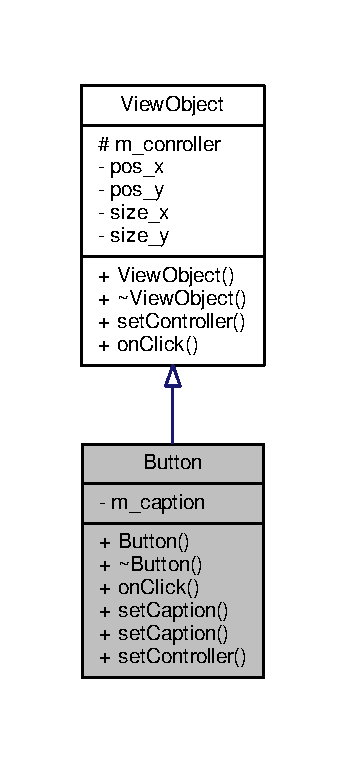
\includegraphics[width=166pt]{class_button__inherit__graph}
\end{center}
\end{figure}


Граф связей класса Button\-:
\nopagebreak
\begin{figure}[H]
\begin{center}
\leavevmode
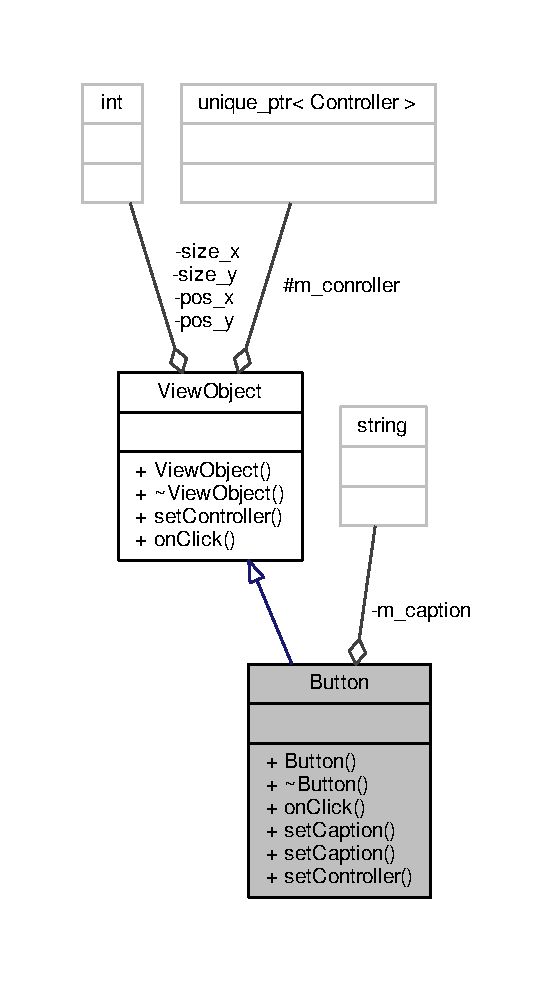
\includegraphics[width=267pt]{class_button__coll__graph}
\end{center}
\end{figure}
\subsection*{Открытые члены}
\begin{DoxyCompactItemize}
\item 
\hyperlink{class_button_ac637a36b28d13a66a0dbce532cec521b}{Button} (const int \&p\-\_\-x, const int \&p\-\_\-y, const int \&s\-\_\-x, const int \&s\-\_\-y)
\item 
\hyperlink{class_button_a2a001eb9c3cc8ae54768a850dd345002}{$\sim$\-Button} ()
\item 
void \hyperlink{class_button_ae0fef75f8dd8a25ae122a379ad330400}{on\-Click} ()
\item 
void \hyperlink{class_button_a95e15fb095da12867e001df39cef24c7}{set\-Caption} (std\-::string \&str)
\item 
void \hyperlink{class_button_ae33b92340f6cd5525c65998452b31260}{set\-Caption} (std\-::string str)
\item 
void \hyperlink{class_button_a2fbc0656e6a74d895365cb4f383b432e}{set\-Controller} (std\-::unique\-\_\-ptr$<$ \hyperlink{class_controller}{Controller} $>$ controller)
\end{DoxyCompactItemize}
\subsection*{Закрытые данные}
\begin{DoxyCompactItemize}
\item 
std\-::string \hyperlink{class_button_a0d3dca4ac1192e87eab73a0f61baf23a}{m\-\_\-caption}
\end{DoxyCompactItemize}
\subsection*{Дополнительные унаследованные члены}


\subsection{Подробное описание}


См. определение в файле v\-\_\-button.\-h строка 10



\subsection{Конструктор(ы)}
\hypertarget{class_button_ac637a36b28d13a66a0dbce532cec521b}{\index{Button@{Button}!Button@{Button}}
\index{Button@{Button}!Button@{Button}}
\subsubsection[{Button}]{\setlength{\rightskip}{0pt plus 5cm}Button\-::\-Button (
\begin{DoxyParamCaption}
\item[{const int \&}]{p\-\_\-x, }
\item[{const int \&}]{p\-\_\-y, }
\item[{const int \&}]{s\-\_\-x, }
\item[{const int \&}]{s\-\_\-y}
\end{DoxyParamCaption}
)\hspace{0.3cm}{\ttfamily [inline]}}}\label{class_button_ac637a36b28d13a66a0dbce532cec521b}


См. определение в файле v\-\_\-button.\-h строка 13

\hypertarget{class_button_a2a001eb9c3cc8ae54768a850dd345002}{\index{Button@{Button}!$\sim$\-Button@{$\sim$\-Button}}
\index{$\sim$\-Button@{$\sim$\-Button}!Button@{Button}}
\subsubsection[{$\sim$\-Button}]{\setlength{\rightskip}{0pt plus 5cm}Button\-::$\sim$\-Button (
\begin{DoxyParamCaption}
{}
\end{DoxyParamCaption}
)\hspace{0.3cm}{\ttfamily [inline]}}}\label{class_button_a2a001eb9c3cc8ae54768a850dd345002}


См. определение в файле v\-\_\-button.\-h строка 14



\subsection{Методы}
\hypertarget{class_button_ae0fef75f8dd8a25ae122a379ad330400}{\index{Button@{Button}!on\-Click@{on\-Click}}
\index{on\-Click@{on\-Click}!Button@{Button}}
\subsubsection[{on\-Click}]{\setlength{\rightskip}{0pt plus 5cm}void Button\-::on\-Click (
\begin{DoxyParamCaption}
{}
\end{DoxyParamCaption}
)\hspace{0.3cm}{\ttfamily [inline]}}}\label{class_button_ae0fef75f8dd8a25ae122a379ad330400}


См. определение в файле v\-\_\-button.\-h строка 15

\hypertarget{class_button_a95e15fb095da12867e001df39cef24c7}{\index{Button@{Button}!set\-Caption@{set\-Caption}}
\index{set\-Caption@{set\-Caption}!Button@{Button}}
\subsubsection[{set\-Caption}]{\setlength{\rightskip}{0pt plus 5cm}void Button\-::set\-Caption (
\begin{DoxyParamCaption}
\item[{std\-::string \&}]{str}
\end{DoxyParamCaption}
)\hspace{0.3cm}{\ttfamily [inline]}}}\label{class_button_a95e15fb095da12867e001df39cef24c7}


См. определение в файле v\-\_\-button.\-h строка 22

\hypertarget{class_button_ae33b92340f6cd5525c65998452b31260}{\index{Button@{Button}!set\-Caption@{set\-Caption}}
\index{set\-Caption@{set\-Caption}!Button@{Button}}
\subsubsection[{set\-Caption}]{\setlength{\rightskip}{0pt plus 5cm}void Button\-::set\-Caption (
\begin{DoxyParamCaption}
\item[{std\-::string}]{str}
\end{DoxyParamCaption}
)\hspace{0.3cm}{\ttfamily [inline]}}}\label{class_button_ae33b92340f6cd5525c65998452b31260}


См. определение в файле v\-\_\-button.\-h строка 23

\hypertarget{class_button_a2fbc0656e6a74d895365cb4f383b432e}{\index{Button@{Button}!set\-Controller@{set\-Controller}}
\index{set\-Controller@{set\-Controller}!Button@{Button}}
\subsubsection[{set\-Controller}]{\setlength{\rightskip}{0pt plus 5cm}void Button\-::set\-Controller (
\begin{DoxyParamCaption}
\item[{std\-::unique\-\_\-ptr$<$ {\bf Controller} $>$}]{controller}
\end{DoxyParamCaption}
)\hspace{0.3cm}{\ttfamily [inline]}}}\label{class_button_a2fbc0656e6a74d895365cb4f383b432e}


См. определение в файле v\-\_\-button.\-h строка 30



\subsection{Данные класса}
\hypertarget{class_button_a0d3dca4ac1192e87eab73a0f61baf23a}{\index{Button@{Button}!m\-\_\-caption@{m\-\_\-caption}}
\index{m\-\_\-caption@{m\-\_\-caption}!Button@{Button}}
\subsubsection[{m\-\_\-caption}]{\setlength{\rightskip}{0pt plus 5cm}std\-::string Button\-::m\-\_\-caption\hspace{0.3cm}{\ttfamily [private]}}}\label{class_button_a0d3dca4ac1192e87eab73a0f61baf23a}


См. определение в файле v\-\_\-button.\-h строка 33



Объявления и описания членов класса находятся в файле\-:\begin{DoxyCompactItemize}
\item 
libs/views/\hyperlink{v__button_8h}{v\-\_\-button.\-h}\end{DoxyCompactItemize}

\hypertarget{class_canvas}{\section{Класс Canvas}
\label{class_canvas}\index{Canvas@{Canvas}}
}


{\ttfamily \#include $<$v\-\_\-canvas.\-h$>$}



Граф наследования\-:Canvas\-:
\nopagebreak
\begin{figure}[H]
\begin{center}
\leavevmode
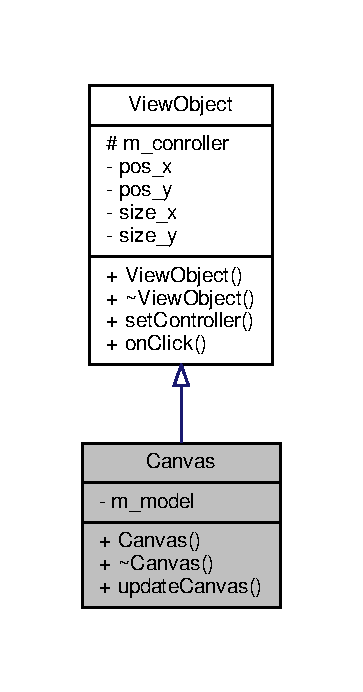
\includegraphics[width=174pt]{class_canvas__inherit__graph}
\end{center}
\end{figure}


Граф связей класса Canvas\-:
\nopagebreak
\begin{figure}[H]
\begin{center}
\leavevmode
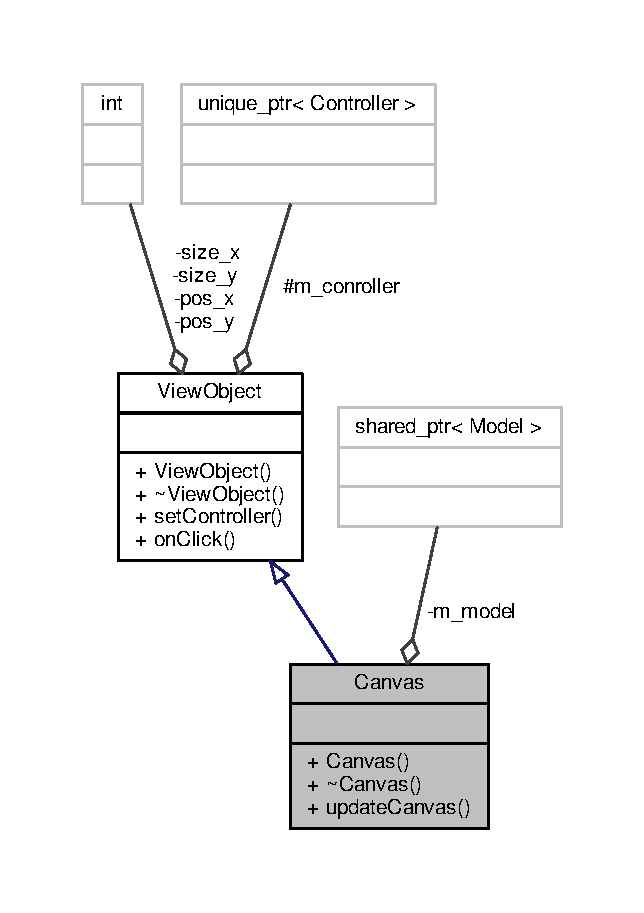
\includegraphics[width=309pt]{class_canvas__coll__graph}
\end{center}
\end{figure}
\subsection*{Открытые члены}
\begin{DoxyCompactItemize}
\item 
\hyperlink{class_canvas_a90a539fde4aa87ad1d09ca220df17c99}{Canvas} (const int \&p\-\_\-x, const int \&p\-\_\-y, const int \&s\-\_\-x, const int \&s\-\_\-y)
\item 
\hyperlink{class_canvas_ac64895ae1cdfc39c58e95097873e861e}{$\sim$\-Canvas} ()=default
\item 
void \hyperlink{class_canvas_a8514b56f7bee6b267dd12b9b11aa97d6}{update\-Canvas} ()
\end{DoxyCompactItemize}
\subsection*{Закрытые данные}
\begin{DoxyCompactItemize}
\item 
std\-::shared\-\_\-ptr$<$ \hyperlink{class_model}{Model} $>$ \hyperlink{class_canvas_a4bae0f13adb834323d28fd1a5884b6e0}{m\-\_\-model}
\end{DoxyCompactItemize}
\subsection*{Дополнительные унаследованные члены}


\subsection{Подробное описание}


См. определение в файле v\-\_\-canvas.\-h строка 6



\subsection{Конструктор(ы)}
\hypertarget{class_canvas_a90a539fde4aa87ad1d09ca220df17c99}{\index{Canvas@{Canvas}!Canvas@{Canvas}}
\index{Canvas@{Canvas}!Canvas@{Canvas}}
\subsubsection[{Canvas}]{\setlength{\rightskip}{0pt plus 5cm}Canvas\-::\-Canvas (
\begin{DoxyParamCaption}
\item[{const int \&}]{p\-\_\-x, }
\item[{const int \&}]{p\-\_\-y, }
\item[{const int \&}]{s\-\_\-x, }
\item[{const int \&}]{s\-\_\-y}
\end{DoxyParamCaption}
)\hspace{0.3cm}{\ttfamily [inline]}}}\label{class_canvas_a90a539fde4aa87ad1d09ca220df17c99}


См. определение в файле v\-\_\-canvas.\-h строка 9

\hypertarget{class_canvas_ac64895ae1cdfc39c58e95097873e861e}{\index{Canvas@{Canvas}!$\sim$\-Canvas@{$\sim$\-Canvas}}
\index{$\sim$\-Canvas@{$\sim$\-Canvas}!Canvas@{Canvas}}
\subsubsection[{$\sim$\-Canvas}]{\setlength{\rightskip}{0pt plus 5cm}Canvas\-::$\sim$\-Canvas (
\begin{DoxyParamCaption}
{}
\end{DoxyParamCaption}
)\hspace{0.3cm}{\ttfamily [default]}}}\label{class_canvas_ac64895ae1cdfc39c58e95097873e861e}


\subsection{Методы}
\hypertarget{class_canvas_a8514b56f7bee6b267dd12b9b11aa97d6}{\index{Canvas@{Canvas}!update\-Canvas@{update\-Canvas}}
\index{update\-Canvas@{update\-Canvas}!Canvas@{Canvas}}
\subsubsection[{update\-Canvas}]{\setlength{\rightskip}{0pt plus 5cm}void Canvas\-::update\-Canvas (
\begin{DoxyParamCaption}
{}
\end{DoxyParamCaption}
)}}\label{class_canvas_a8514b56f7bee6b267dd12b9b11aa97d6}


\subsection{Данные класса}
\hypertarget{class_canvas_a4bae0f13adb834323d28fd1a5884b6e0}{\index{Canvas@{Canvas}!m\-\_\-model@{m\-\_\-model}}
\index{m\-\_\-model@{m\-\_\-model}!Canvas@{Canvas}}
\subsubsection[{m\-\_\-model}]{\setlength{\rightskip}{0pt plus 5cm}std\-::shared\-\_\-ptr$<${\bf Model}$>$ Canvas\-::m\-\_\-model\hspace{0.3cm}{\ttfamily [private]}}}\label{class_canvas_a4bae0f13adb834323d28fd1a5884b6e0}


См. определение в файле v\-\_\-canvas.\-h строка 15



Объявления и описания членов класса находятся в файле\-:\begin{DoxyCompactItemize}
\item 
libs/views/\hyperlink{v__canvas_8h}{v\-\_\-canvas.\-h}\end{DoxyCompactItemize}

\hypertarget{class_controller}{\section{Класс Controller}
\label{class_controller}\index{Controller@{Controller}}
}


{\ttfamily \#include $<$base\-Controller.\-h$>$}



Граф наследования\-:Controller\-:
\nopagebreak
\begin{figure}[H]
\begin{center}
\leavevmode
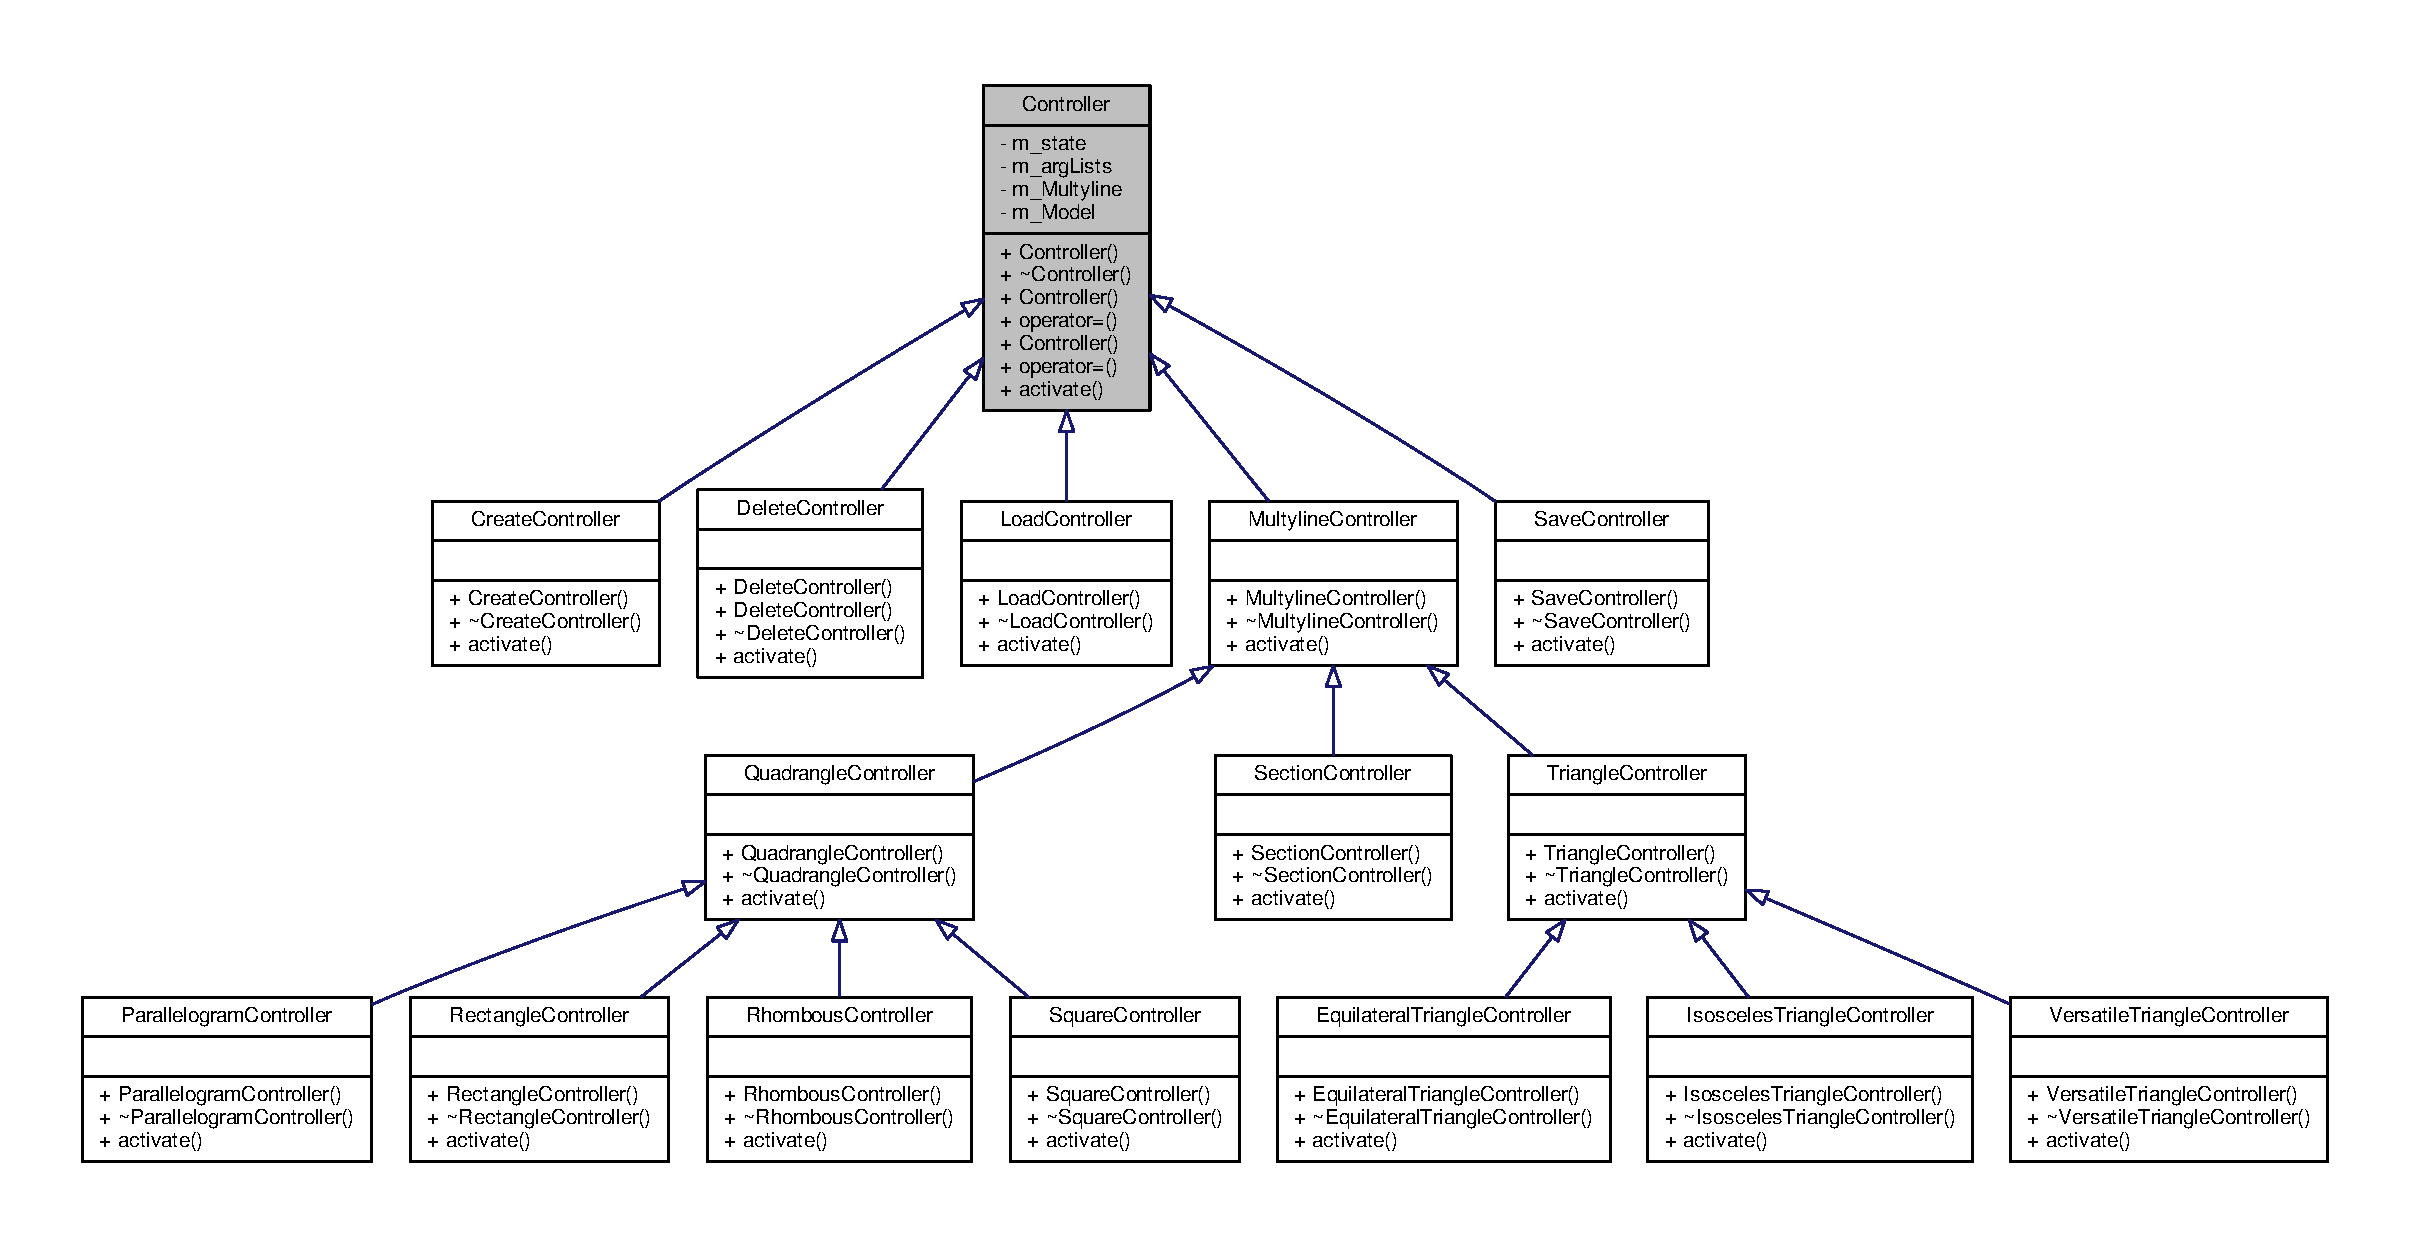
\includegraphics[width=350pt]{class_controller__inherit__graph}
\end{center}
\end{figure}


Граф связей класса Controller\-:
\nopagebreak
\begin{figure}[H]
\begin{center}
\leavevmode
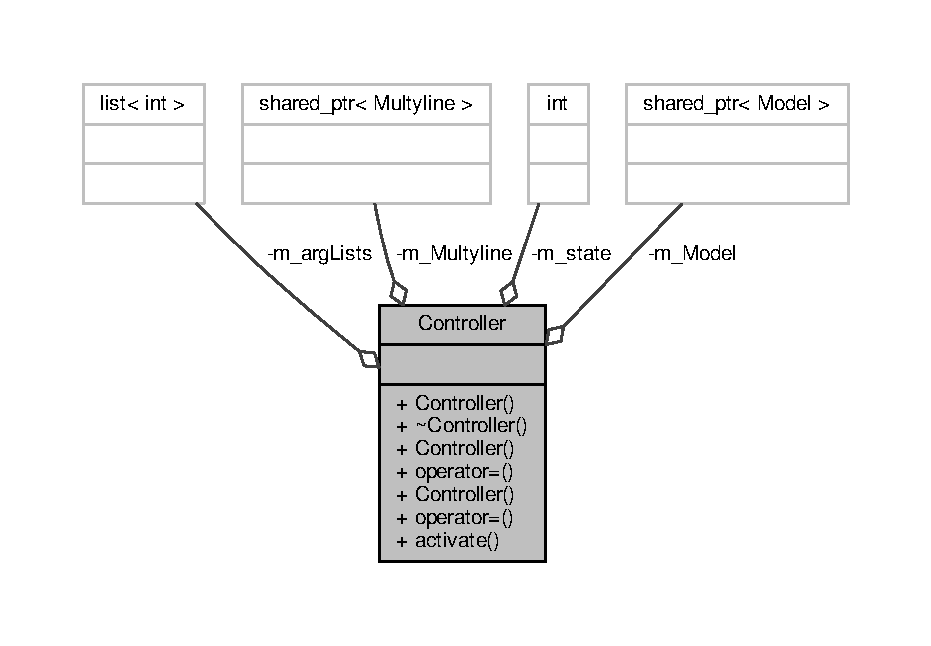
\includegraphics[width=350pt]{class_controller__coll__graph}
\end{center}
\end{figure}
\subsection*{Открытые члены}
\begin{DoxyCompactItemize}
\item 
\hyperlink{class_controller_ad2ce690a1bfa8ec80e9785ee8b475592}{Controller} (std\-::shared\-\_\-ptr$<$ \hyperlink{class_model}{Model} $>$ \&model)
\item 
virtual \hyperlink{class_controller_a8d16a7a97c266dc0d5aa5685c4dcdd89}{$\sim$\-Controller} ()=default
\item 
\hyperlink{class_controller_abae5d6be388bd2499f1ffb01a4c60f2d}{Controller} (\hyperlink{class_controller}{Controller} \&other)
\item 
\hyperlink{class_controller}{Controller} \& \hyperlink{class_controller_a74985f0bdefdb90a5d31e195684aac97}{operator=} (\hyperlink{class_controller}{Controller} \&other)
\item 
\hyperlink{class_controller_a8b96e5f809484c765067f551e948b32a}{Controller} (\hyperlink{class_controller}{Controller} \&\&other)
\item 
\hyperlink{class_controller}{Controller} \& \hyperlink{class_controller_a9b263660c90a6d2f7e65ccadaa46fd2d}{operator=} (\hyperlink{class_controller}{Controller} \&\&other)
\item 
virtual void \hyperlink{class_controller_a4cc69a630011f49efb0c221d617af633}{activate} (int cursor\-Pos\-X, int cursor\-Pos\-Y)=0
\end{DoxyCompactItemize}
\subsection*{Закрытые данные}
\begin{DoxyCompactItemize}
\item 
int \hyperlink{class_controller_a8b090b5fb29c22eb74d6bab24713ce4e}{m\-\_\-state}
\item 
std\-::list$<$ int $>$ \hyperlink{class_controller_acaa49bf804d980462e65b7c9df8228ad}{m\-\_\-arg\-Lists}
\item 
std\-::shared\-\_\-ptr$<$ \hyperlink{class_multyline}{Multyline} $>$ \hyperlink{class_controller_a58633f078953ff4035c7fd1fc14ba01c}{m\-\_\-\-Multyline}
\item 
std\-::shared\-\_\-ptr$<$ \hyperlink{class_model}{Model} $>$ \hyperlink{class_controller_a5190c0bded8b780fed2baaf56737b9cb}{m\-\_\-\-Model}
\end{DoxyCompactItemize}


\subsection{Подробное описание}


См. определение в файле base\-Controller.\-h строка 7



\subsection{Конструктор(ы)}
\hypertarget{class_controller_ad2ce690a1bfa8ec80e9785ee8b475592}{\index{Controller@{Controller}!Controller@{Controller}}
\index{Controller@{Controller}!Controller@{Controller}}
\subsubsection[{Controller}]{\setlength{\rightskip}{0pt plus 5cm}Controller\-::\-Controller (
\begin{DoxyParamCaption}
\item[{std\-::shared\-\_\-ptr$<$ {\bf Model} $>$ \&}]{model}
\end{DoxyParamCaption}
)\hspace{0.3cm}{\ttfamily [inline]}}}\label{class_controller_ad2ce690a1bfa8ec80e9785ee8b475592}


См. определение в файле base\-Controller.\-h строка 10

\hypertarget{class_controller_a8d16a7a97c266dc0d5aa5685c4dcdd89}{\index{Controller@{Controller}!$\sim$\-Controller@{$\sim$\-Controller}}
\index{$\sim$\-Controller@{$\sim$\-Controller}!Controller@{Controller}}
\subsubsection[{$\sim$\-Controller}]{\setlength{\rightskip}{0pt plus 5cm}virtual Controller\-::$\sim$\-Controller (
\begin{DoxyParamCaption}
{}
\end{DoxyParamCaption}
)\hspace{0.3cm}{\ttfamily [virtual]}, {\ttfamily [default]}}}\label{class_controller_a8d16a7a97c266dc0d5aa5685c4dcdd89}
\hypertarget{class_controller_abae5d6be388bd2499f1ffb01a4c60f2d}{\index{Controller@{Controller}!Controller@{Controller}}
\index{Controller@{Controller}!Controller@{Controller}}
\subsubsection[{Controller}]{\setlength{\rightskip}{0pt plus 5cm}Controller\-::\-Controller (
\begin{DoxyParamCaption}
\item[{{\bf Controller} \&}]{other}
\end{DoxyParamCaption}
)}}\label{class_controller_abae5d6be388bd2499f1ffb01a4c60f2d}
\hypertarget{class_controller_a8b96e5f809484c765067f551e948b32a}{\index{Controller@{Controller}!Controller@{Controller}}
\index{Controller@{Controller}!Controller@{Controller}}
\subsubsection[{Controller}]{\setlength{\rightskip}{0pt plus 5cm}Controller\-::\-Controller (
\begin{DoxyParamCaption}
\item[{{\bf Controller} \&\&}]{other}
\end{DoxyParamCaption}
)}}\label{class_controller_a8b96e5f809484c765067f551e948b32a}


\subsection{Методы}
\hypertarget{class_controller_a4cc69a630011f49efb0c221d617af633}{\index{Controller@{Controller}!activate@{activate}}
\index{activate@{activate}!Controller@{Controller}}
\subsubsection[{activate}]{\setlength{\rightskip}{0pt plus 5cm}void Controller\-::activate (
\begin{DoxyParamCaption}
\item[{int}]{cursor\-Pos\-X, }
\item[{int}]{cursor\-Pos\-Y}
\end{DoxyParamCaption}
)\hspace{0.3cm}{\ttfamily [pure virtual]}}}\label{class_controller_a4cc69a630011f49efb0c221d617af633}


Замещается в \hyperlink{class_parallelogram_controller_a42022d7939a32ef5fcdced235edad018}{Parallelogram\-Controller}, \hyperlink{class_rhombous_controller_a9e839123b8a65d202fb898b6233694b2}{Rhombous\-Controller}, \hyperlink{class_rectangle_controller_ac0d209fecccce59cf9270f7f6facbc06}{Rectangle\-Controller}, \hyperlink{class_square_controller_a169d59d75dd023ed352e7722a3bd2dcc}{Square\-Controller}, \hyperlink{class_quadrangle_controller_a2a38c3afba85014f27041e002cfc7950}{Quadrangle\-Controller}, \hyperlink{class_equilateral_triangle_controller_ac8822ad6419def097652fc8a88426898}{Equilateral\-Triangle\-Controller}, \hyperlink{class_isosceles_triangle_controller_ac060b7bdfdc3c5fc078147e14e31415b}{Isosceles\-Triangle\-Controller}, \hyperlink{class_versatile_triangle_controller_a0d553f2393114a789f3e3964b97dad66}{Versatile\-Triangle\-Controller}, \hyperlink{class_triangle_controller_ab86471e4de39ae99bc6198583d173c7b}{Triangle\-Controller}, \hyperlink{class_section_controller_ac42bb71f574f336a79a2e0a739fbad24}{Section\-Controller}, \hyperlink{class_multyline_controller_a5a574a5ca48d2a7e62201e9415a61afe}{Multyline\-Controller}, \hyperlink{class_delete_controller_a77305d1d2c625ff61b61f97a8beffd03}{Delete\-Controller}, \hyperlink{class_save_controller_a82d91ea99368d4cbce96a24d988a8c2b}{Save\-Controller}, \hyperlink{class_load_controller_aa9fc9b866ea0abda7d8d766ffa9256f4}{Load\-Controller} и \hyperlink{class_create_controller_abc72a0a1947c1dd5eec2cdfd84f481c5}{Create\-Controller}.



См. определение в файле base\-Controller.\-h строка 28

\hypertarget{class_controller_a74985f0bdefdb90a5d31e195684aac97}{\index{Controller@{Controller}!operator=@{operator=}}
\index{operator=@{operator=}!Controller@{Controller}}
\subsubsection[{operator=}]{\setlength{\rightskip}{0pt plus 5cm}{\bf Controller}\& Controller\-::operator= (
\begin{DoxyParamCaption}
\item[{{\bf Controller} \&}]{other}
\end{DoxyParamCaption}
)}}\label{class_controller_a74985f0bdefdb90a5d31e195684aac97}
\hypertarget{class_controller_a9b263660c90a6d2f7e65ccadaa46fd2d}{\index{Controller@{Controller}!operator=@{operator=}}
\index{operator=@{operator=}!Controller@{Controller}}
\subsubsection[{operator=}]{\setlength{\rightskip}{0pt plus 5cm}{\bf Controller}\& Controller\-::operator= (
\begin{DoxyParamCaption}
\item[{{\bf Controller} \&\&}]{other}
\end{DoxyParamCaption}
)}}\label{class_controller_a9b263660c90a6d2f7e65ccadaa46fd2d}


\subsection{Данные класса}
\hypertarget{class_controller_acaa49bf804d980462e65b7c9df8228ad}{\index{Controller@{Controller}!m\-\_\-arg\-Lists@{m\-\_\-arg\-Lists}}
\index{m\-\_\-arg\-Lists@{m\-\_\-arg\-Lists}!Controller@{Controller}}
\subsubsection[{m\-\_\-arg\-Lists}]{\setlength{\rightskip}{0pt plus 5cm}std\-::list$<$int$>$ Controller\-::m\-\_\-arg\-Lists\hspace{0.3cm}{\ttfamily [private]}}}\label{class_controller_acaa49bf804d980462e65b7c9df8228ad}


См. определение в файле base\-Controller.\-h строка 22

\hypertarget{class_controller_a5190c0bded8b780fed2baaf56737b9cb}{\index{Controller@{Controller}!m\-\_\-\-Model@{m\-\_\-\-Model}}
\index{m\-\_\-\-Model@{m\-\_\-\-Model}!Controller@{Controller}}
\subsubsection[{m\-\_\-\-Model}]{\setlength{\rightskip}{0pt plus 5cm}std\-::shared\-\_\-ptr$<${\bf Model}$>$ Controller\-::m\-\_\-\-Model\hspace{0.3cm}{\ttfamily [private]}}}\label{class_controller_a5190c0bded8b780fed2baaf56737b9cb}


См. определение в файле base\-Controller.\-h строка 24

\hypertarget{class_controller_a58633f078953ff4035c7fd1fc14ba01c}{\index{Controller@{Controller}!m\-\_\-\-Multyline@{m\-\_\-\-Multyline}}
\index{m\-\_\-\-Multyline@{m\-\_\-\-Multyline}!Controller@{Controller}}
\subsubsection[{m\-\_\-\-Multyline}]{\setlength{\rightskip}{0pt plus 5cm}std\-::shared\-\_\-ptr$<${\bf Multyline}$>$ Controller\-::m\-\_\-\-Multyline\hspace{0.3cm}{\ttfamily [private]}}}\label{class_controller_a58633f078953ff4035c7fd1fc14ba01c}


См. определение в файле base\-Controller.\-h строка 23

\hypertarget{class_controller_a8b090b5fb29c22eb74d6bab24713ce4e}{\index{Controller@{Controller}!m\-\_\-state@{m\-\_\-state}}
\index{m\-\_\-state@{m\-\_\-state}!Controller@{Controller}}
\subsubsection[{m\-\_\-state}]{\setlength{\rightskip}{0pt plus 5cm}int Controller\-::m\-\_\-state\hspace{0.3cm}{\ttfamily [private]}}}\label{class_controller_a8b090b5fb29c22eb74d6bab24713ce4e}


См. определение в файле base\-Controller.\-h строка 21



Объявления и описания членов класса находятся в файле\-:\begin{DoxyCompactItemize}
\item 
libs/controllers/\hyperlink{base_controller_8h}{base\-Controller.\-h}\end{DoxyCompactItemize}

\hypertarget{class_create_controller}{\section{Класс Create\-Controller}
\label{class_create_controller}\index{Create\-Controller@{Create\-Controller}}
}


{\ttfamily \#include $<$base\-Controller.\-h$>$}



Граф наследования\-:Create\-Controller\-:
\nopagebreak
\begin{figure}[H]
\begin{center}
\leavevmode
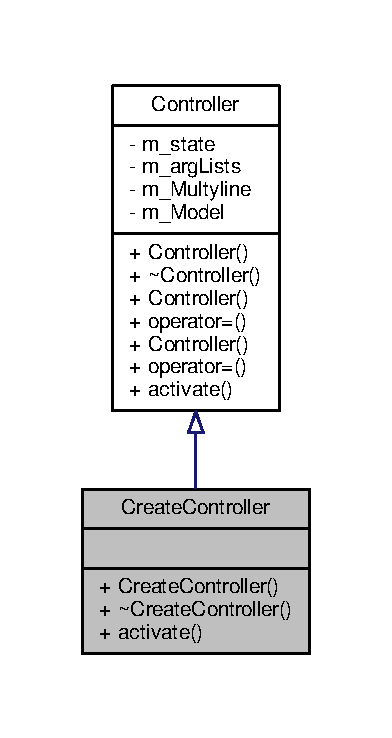
\includegraphics[width=188pt]{class_create_controller__inherit__graph}
\end{center}
\end{figure}


Граф связей класса Create\-Controller\-:
\nopagebreak
\begin{figure}[H]
\begin{center}
\leavevmode
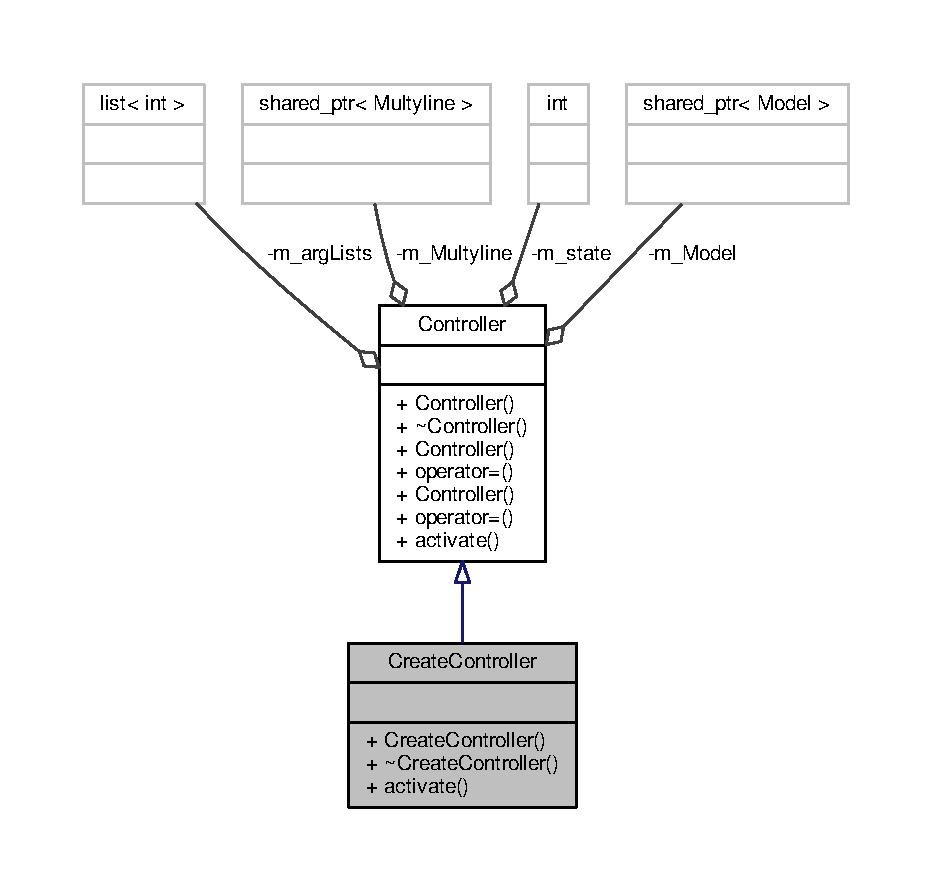
\includegraphics[width=350pt]{class_create_controller__coll__graph}
\end{center}
\end{figure}
\subsection*{Открытые члены}
\begin{DoxyCompactItemize}
\item 
\hyperlink{class_create_controller_a5d544e80e4786ae8767b61b8fa303f5f}{Create\-Controller} (std\-::shared\-\_\-ptr$<$ \hyperlink{class_model}{Model} $>$ \&model)
\item 
\hyperlink{class_create_controller_af894a8921fb37dec129fc22f9bc6a86a}{$\sim$\-Create\-Controller} ()=default
\item 
void \hyperlink{class_create_controller_abc72a0a1947c1dd5eec2cdfd84f481c5}{activate} (int cursor\-Pos\-X, int cursor\-Pos\-Y) final
\end{DoxyCompactItemize}


\subsection{Подробное описание}


См. определение в файле base\-Controller.\-h строка 35



\subsection{Конструктор(ы)}
\hypertarget{class_create_controller_a5d544e80e4786ae8767b61b8fa303f5f}{\index{Create\-Controller@{Create\-Controller}!Create\-Controller@{Create\-Controller}}
\index{Create\-Controller@{Create\-Controller}!CreateController@{Create\-Controller}}
\subsubsection[{Create\-Controller}]{\setlength{\rightskip}{0pt plus 5cm}Create\-Controller\-::\-Create\-Controller (
\begin{DoxyParamCaption}
\item[{std\-::shared\-\_\-ptr$<$ {\bf Model} $>$ \&}]{model}
\end{DoxyParamCaption}
)\hspace{0.3cm}{\ttfamily [inline]}}}\label{class_create_controller_a5d544e80e4786ae8767b61b8fa303f5f}


См. определение в файле base\-Controller.\-h строка 38

\hypertarget{class_create_controller_af894a8921fb37dec129fc22f9bc6a86a}{\index{Create\-Controller@{Create\-Controller}!$\sim$\-Create\-Controller@{$\sim$\-Create\-Controller}}
\index{$\sim$\-Create\-Controller@{$\sim$\-Create\-Controller}!CreateController@{Create\-Controller}}
\subsubsection[{$\sim$\-Create\-Controller}]{\setlength{\rightskip}{0pt plus 5cm}Create\-Controller\-::$\sim$\-Create\-Controller (
\begin{DoxyParamCaption}
{}
\end{DoxyParamCaption}
)\hspace{0.3cm}{\ttfamily [default]}}}\label{class_create_controller_af894a8921fb37dec129fc22f9bc6a86a}


\subsection{Методы}
\hypertarget{class_create_controller_abc72a0a1947c1dd5eec2cdfd84f481c5}{\index{Create\-Controller@{Create\-Controller}!activate@{activate}}
\index{activate@{activate}!CreateController@{Create\-Controller}}
\subsubsection[{activate}]{\setlength{\rightskip}{0pt plus 5cm}void Create\-Controller\-::activate (
\begin{DoxyParamCaption}
\item[{int}]{cursor\-Pos\-X, }
\item[{int}]{cursor\-Pos\-Y}
\end{DoxyParamCaption}
)\hspace{0.3cm}{\ttfamily [inline]}, {\ttfamily [final]}, {\ttfamily [virtual]}}}\label{class_create_controller_abc72a0a1947c1dd5eec2cdfd84f481c5}


Замещает \hyperlink{class_controller_a4cc69a630011f49efb0c221d617af633}{Controller}.



См. определение в файле base\-Controller.\-h строка 40



Объявления и описания членов класса находятся в файле\-:\begin{DoxyCompactItemize}
\item 
libs/controllers/\hyperlink{base_controller_8h}{base\-Controller.\-h}\end{DoxyCompactItemize}

\hypertarget{class_delete_controller}{\section{Класс Delete\-Controller}
\label{class_delete_controller}\index{Delete\-Controller@{Delete\-Controller}}
}


{\ttfamily \#include $<$base\-Controller.\-h$>$}



Граф наследования\-:Delete\-Controller\-:
\nopagebreak
\begin{figure}[H]
\begin{center}
\leavevmode
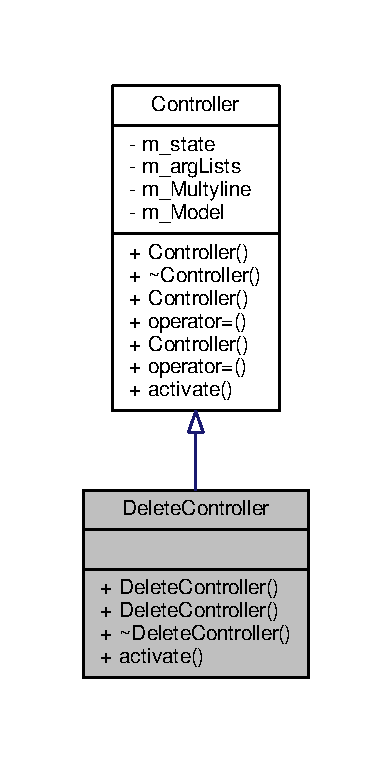
\includegraphics[width=188pt]{class_delete_controller__inherit__graph}
\end{center}
\end{figure}


Граф связей класса Delete\-Controller\-:
\nopagebreak
\begin{figure}[H]
\begin{center}
\leavevmode
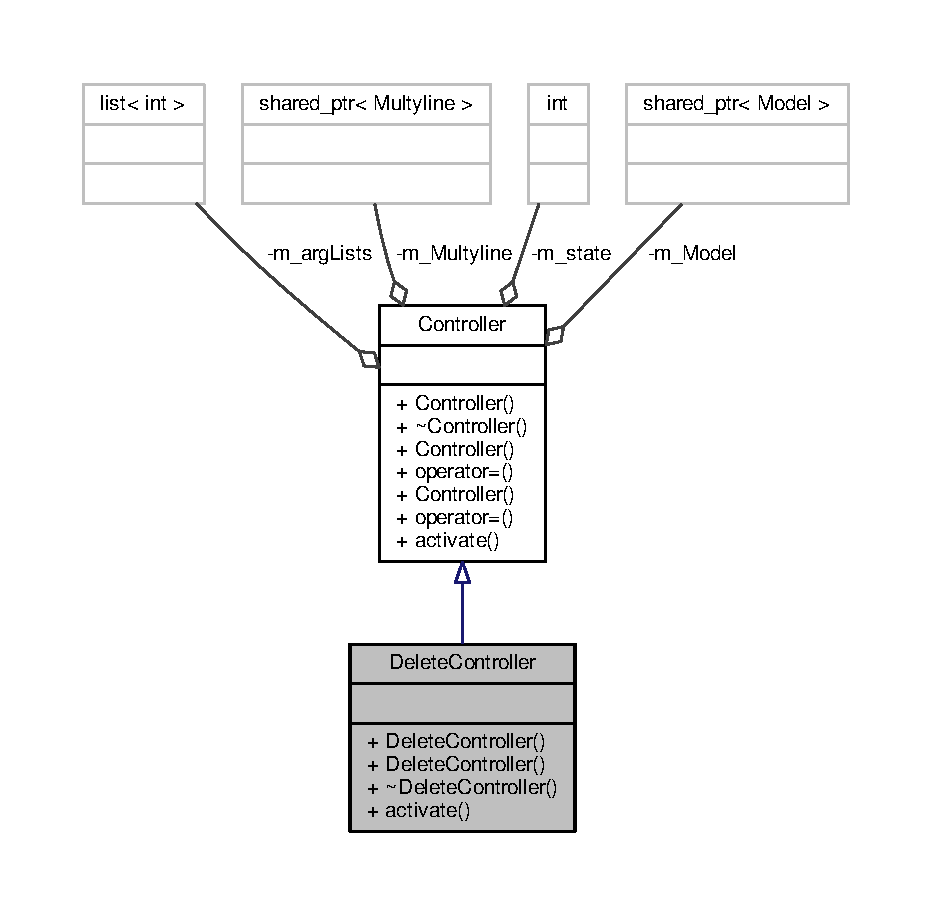
\includegraphics[width=350pt]{class_delete_controller__coll__graph}
\end{center}
\end{figure}
\subsection*{Открытые члены}
\begin{DoxyCompactItemize}
\item 
\hyperlink{class_delete_controller_acaa7ec19df8914bad38a2119e0a69ba9}{Delete\-Controller} ()=delete
\item 
\hyperlink{class_delete_controller_ae51255a8c23649c9bcd024a43a254129}{Delete\-Controller} (std\-::shared\-\_\-ptr$<$ \hyperlink{class_model}{Model} $>$ \&model)
\item 
\hyperlink{class_delete_controller_a1ea8fdb189618aa6c305a27e48f059f9}{$\sim$\-Delete\-Controller} ()=default
\item 
void \hyperlink{class_delete_controller_a77305d1d2c625ff61b61f97a8beffd03}{activate} (int cursor\-Pos\-X, int cursor\-Pos\-Y) final
\end{DoxyCompactItemize}


\subsection{Подробное описание}


См. определение в файле base\-Controller.\-h строка 74



\subsection{Конструктор(ы)}
\hypertarget{class_delete_controller_acaa7ec19df8914bad38a2119e0a69ba9}{\index{Delete\-Controller@{Delete\-Controller}!Delete\-Controller@{Delete\-Controller}}
\index{Delete\-Controller@{Delete\-Controller}!DeleteController@{Delete\-Controller}}
\subsubsection[{Delete\-Controller}]{\setlength{\rightskip}{0pt plus 5cm}Delete\-Controller\-::\-Delete\-Controller (
\begin{DoxyParamCaption}
{}
\end{DoxyParamCaption}
)\hspace{0.3cm}{\ttfamily [delete]}}}\label{class_delete_controller_acaa7ec19df8914bad38a2119e0a69ba9}
\hypertarget{class_delete_controller_ae51255a8c23649c9bcd024a43a254129}{\index{Delete\-Controller@{Delete\-Controller}!Delete\-Controller@{Delete\-Controller}}
\index{Delete\-Controller@{Delete\-Controller}!DeleteController@{Delete\-Controller}}
\subsubsection[{Delete\-Controller}]{\setlength{\rightskip}{0pt plus 5cm}Delete\-Controller\-::\-Delete\-Controller (
\begin{DoxyParamCaption}
\item[{std\-::shared\-\_\-ptr$<$ {\bf Model} $>$ \&}]{model}
\end{DoxyParamCaption}
)\hspace{0.3cm}{\ttfamily [inline]}}}\label{class_delete_controller_ae51255a8c23649c9bcd024a43a254129}


См. определение в файле base\-Controller.\-h строка 78

\hypertarget{class_delete_controller_a1ea8fdb189618aa6c305a27e48f059f9}{\index{Delete\-Controller@{Delete\-Controller}!$\sim$\-Delete\-Controller@{$\sim$\-Delete\-Controller}}
\index{$\sim$\-Delete\-Controller@{$\sim$\-Delete\-Controller}!DeleteController@{Delete\-Controller}}
\subsubsection[{$\sim$\-Delete\-Controller}]{\setlength{\rightskip}{0pt plus 5cm}Delete\-Controller\-::$\sim$\-Delete\-Controller (
\begin{DoxyParamCaption}
{}
\end{DoxyParamCaption}
)\hspace{0.3cm}{\ttfamily [default]}}}\label{class_delete_controller_a1ea8fdb189618aa6c305a27e48f059f9}


\subsection{Методы}
\hypertarget{class_delete_controller_a77305d1d2c625ff61b61f97a8beffd03}{\index{Delete\-Controller@{Delete\-Controller}!activate@{activate}}
\index{activate@{activate}!DeleteController@{Delete\-Controller}}
\subsubsection[{activate}]{\setlength{\rightskip}{0pt plus 5cm}void Delete\-Controller\-::activate (
\begin{DoxyParamCaption}
\item[{int}]{cursor\-Pos\-X, }
\item[{int}]{cursor\-Pos\-Y}
\end{DoxyParamCaption}
)\hspace{0.3cm}{\ttfamily [inline]}, {\ttfamily [final]}, {\ttfamily [virtual]}}}\label{class_delete_controller_a77305d1d2c625ff61b61f97a8beffd03}


Замещает \hyperlink{class_controller_a4cc69a630011f49efb0c221d617af633}{Controller}.



См. определение в файле base\-Controller.\-h строка 80



Объявления и описания членов класса находятся в файле\-:\begin{DoxyCompactItemize}
\item 
libs/controllers/\hyperlink{base_controller_8h}{base\-Controller.\-h}\end{DoxyCompactItemize}

\hypertarget{class_equilateral_triangle}{\section{Класс Equilateral\-Triangle}
\label{class_equilateral_triangle}\index{Equilateral\-Triangle@{Equilateral\-Triangle}}
}


{\ttfamily \#include $<$m3\-\_\-basic.\-h$>$}



Граф наследования\-:Equilateral\-Triangle\-:
\nopagebreak
\begin{figure}[H]
\begin{center}
\leavevmode
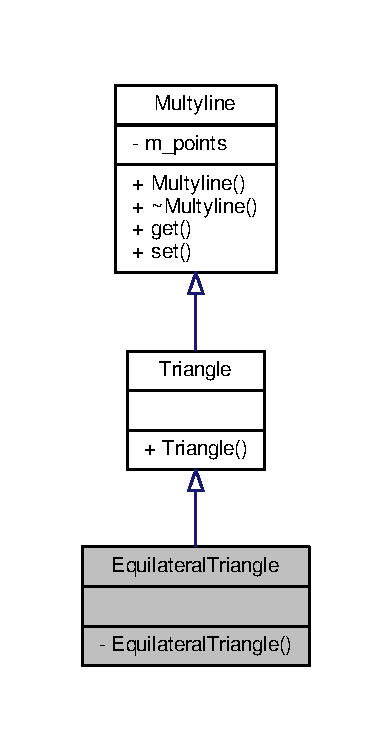
\includegraphics[width=188pt]{class_equilateral_triangle__inherit__graph}
\end{center}
\end{figure}


Граф связей класса Equilateral\-Triangle\-:
\nopagebreak
\begin{figure}[H]
\begin{center}
\leavevmode
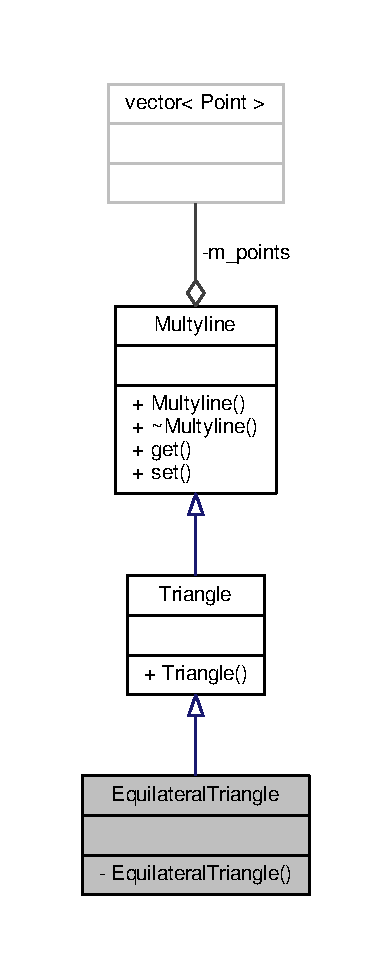
\includegraphics[width=188pt]{class_equilateral_triangle__coll__graph}
\end{center}
\end{figure}
\subsection*{Закрытые типы}
\begin{DoxyCompactItemize}
\item 
enum \hyperlink{class_equilateral_triangle_a9ddc7a249c2c1cc8f4c5fabc0638f207}{calc\-Method} \{ \hyperlink{class_equilateral_triangle_a9ddc7a249c2c1cc8f4c5fabc0638f207ab22c1ea5ea1ee25fa8afd9400de5c297}{point1side}, 
\hyperlink{class_equilateral_triangle_a9ddc7a249c2c1cc8f4c5fabc0638f207a031108bfa10203230179e8ba4b5070ab}{mid\-Base}, 
\hyperlink{class_equilateral_triangle_a9ddc7a249c2c1cc8f4c5fabc0638f207a108152f513b3929e8f8923d156ee59e5}{mid3}
 \}
\end{DoxyCompactItemize}
\subsection*{Закрытые члены}
\begin{DoxyCompactItemize}
\item 
\hyperlink{class_equilateral_triangle_a62872b42bd79252e40d9f4acf1b347bf}{Equilateral\-Triangle} (\hyperlink{class_equilateral_triangle_a9ddc7a249c2c1cc8f4c5fabc0638f207}{calc\-Method}, std\-::initializer\-\_\-list$<$ double $>$ \&)
\end{DoxyCompactItemize}
\subsection*{Дополнительные унаследованные члены}


\subsection{Подробное описание}


См. определение в файле m3\-\_\-basic.\-h строка 64



\subsection{Перечисления}
\hypertarget{class_equilateral_triangle_a9ddc7a249c2c1cc8f4c5fabc0638f207}{\index{Equilateral\-Triangle@{Equilateral\-Triangle}!calc\-Method@{calc\-Method}}
\index{calc\-Method@{calc\-Method}!EquilateralTriangle@{Equilateral\-Triangle}}
\subsubsection[{calc\-Method}]{\setlength{\rightskip}{0pt plus 5cm}enum {\bf Equilateral\-Triangle\-::calc\-Method}\hspace{0.3cm}{\ttfamily [private]}}}\label{class_equilateral_triangle_a9ddc7a249c2c1cc8f4c5fabc0638f207}
\begin{Desc}
\item[Элементы перечислений]\par
\begin{description}
\index{point1side@{point1side}!Equilateral\-Triangle@{Equilateral\-Triangle}}\index{Equilateral\-Triangle@{Equilateral\-Triangle}!point1side@{point1side}}\item[{\em 
\hypertarget{class_equilateral_triangle_a9ddc7a249c2c1cc8f4c5fabc0638f207ab22c1ea5ea1ee25fa8afd9400de5c297}{point1side}\label{class_equilateral_triangle_a9ddc7a249c2c1cc8f4c5fabc0638f207ab22c1ea5ea1ee25fa8afd9400de5c297}
}]\index{mid\-Base@{mid\-Base}!Equilateral\-Triangle@{Equilateral\-Triangle}}\index{Equilateral\-Triangle@{Equilateral\-Triangle}!mid\-Base@{mid\-Base}}\item[{\em 
\hypertarget{class_equilateral_triangle_a9ddc7a249c2c1cc8f4c5fabc0638f207a031108bfa10203230179e8ba4b5070ab}{mid\-Base}\label{class_equilateral_triangle_a9ddc7a249c2c1cc8f4c5fabc0638f207a031108bfa10203230179e8ba4b5070ab}
}]\index{mid3@{mid3}!Equilateral\-Triangle@{Equilateral\-Triangle}}\index{Equilateral\-Triangle@{Equilateral\-Triangle}!mid3@{mid3}}\item[{\em 
\hypertarget{class_equilateral_triangle_a9ddc7a249c2c1cc8f4c5fabc0638f207a108152f513b3929e8f8923d156ee59e5}{mid3}\label{class_equilateral_triangle_a9ddc7a249c2c1cc8f4c5fabc0638f207a108152f513b3929e8f8923d156ee59e5}
}]\end{description}
\end{Desc}


См. определение в файле m3\-\_\-basic.\-h строка 66



\subsection{Конструктор(ы)}
\hypertarget{class_equilateral_triangle_a62872b42bd79252e40d9f4acf1b347bf}{\index{Equilateral\-Triangle@{Equilateral\-Triangle}!Equilateral\-Triangle@{Equilateral\-Triangle}}
\index{Equilateral\-Triangle@{Equilateral\-Triangle}!EquilateralTriangle@{Equilateral\-Triangle}}
\subsubsection[{Equilateral\-Triangle}]{\setlength{\rightskip}{0pt plus 5cm}Equilateral\-Triangle\-::\-Equilateral\-Triangle (
\begin{DoxyParamCaption}
\item[{{\bf calc\-Method}}]{, }
\item[{std\-::initializer\-\_\-list$<$ double $>$ \&}]{}
\end{DoxyParamCaption}
)\hspace{0.3cm}{\ttfamily [private]}}}\label{class_equilateral_triangle_a62872b42bd79252e40d9f4acf1b347bf}


Объявления и описания членов класса находятся в файле\-:\begin{DoxyCompactItemize}
\item 
libs/models/m\-\_\-shapes/\hyperlink{m3__basic_8h}{m3\-\_\-basic.\-h}\end{DoxyCompactItemize}

\hypertarget{class_equilateral_triangle_controller}{\section{Класс Equilateral\-Triangle\-Controller}
\label{class_equilateral_triangle_controller}\index{Equilateral\-Triangle\-Controller@{Equilateral\-Triangle\-Controller}}
}


{\ttfamily \#include $<$base\-Controller.\-h$>$}



Граф наследования\-:Equilateral\-Triangle\-Controller\-:
\nopagebreak
\begin{figure}[H]
\begin{center}
\leavevmode
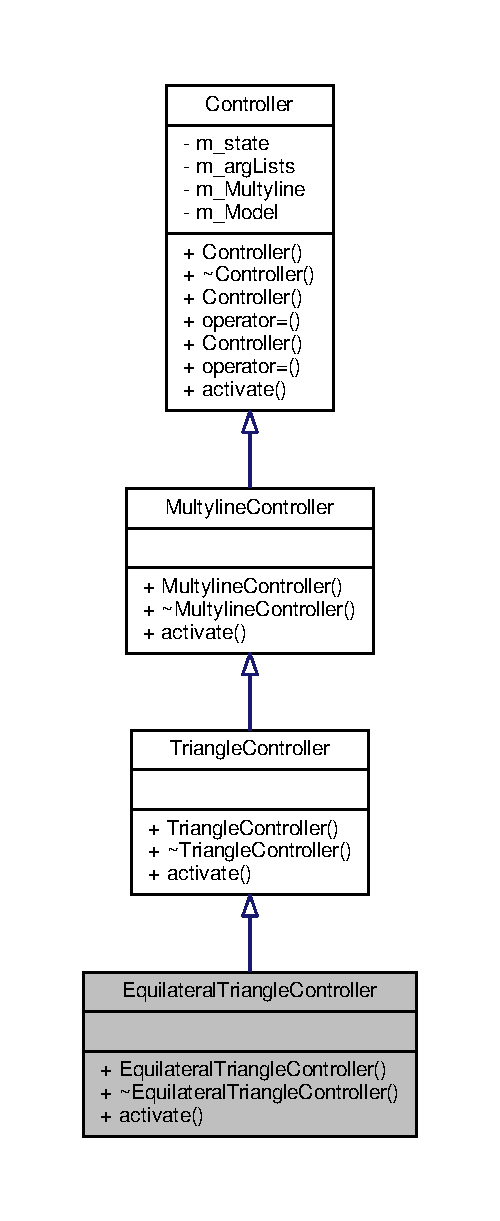
\includegraphics[height=550pt]{class_equilateral_triangle_controller__inherit__graph}
\end{center}
\end{figure}


Граф связей класса Equilateral\-Triangle\-Controller\-:
\nopagebreak
\begin{figure}[H]
\begin{center}
\leavevmode
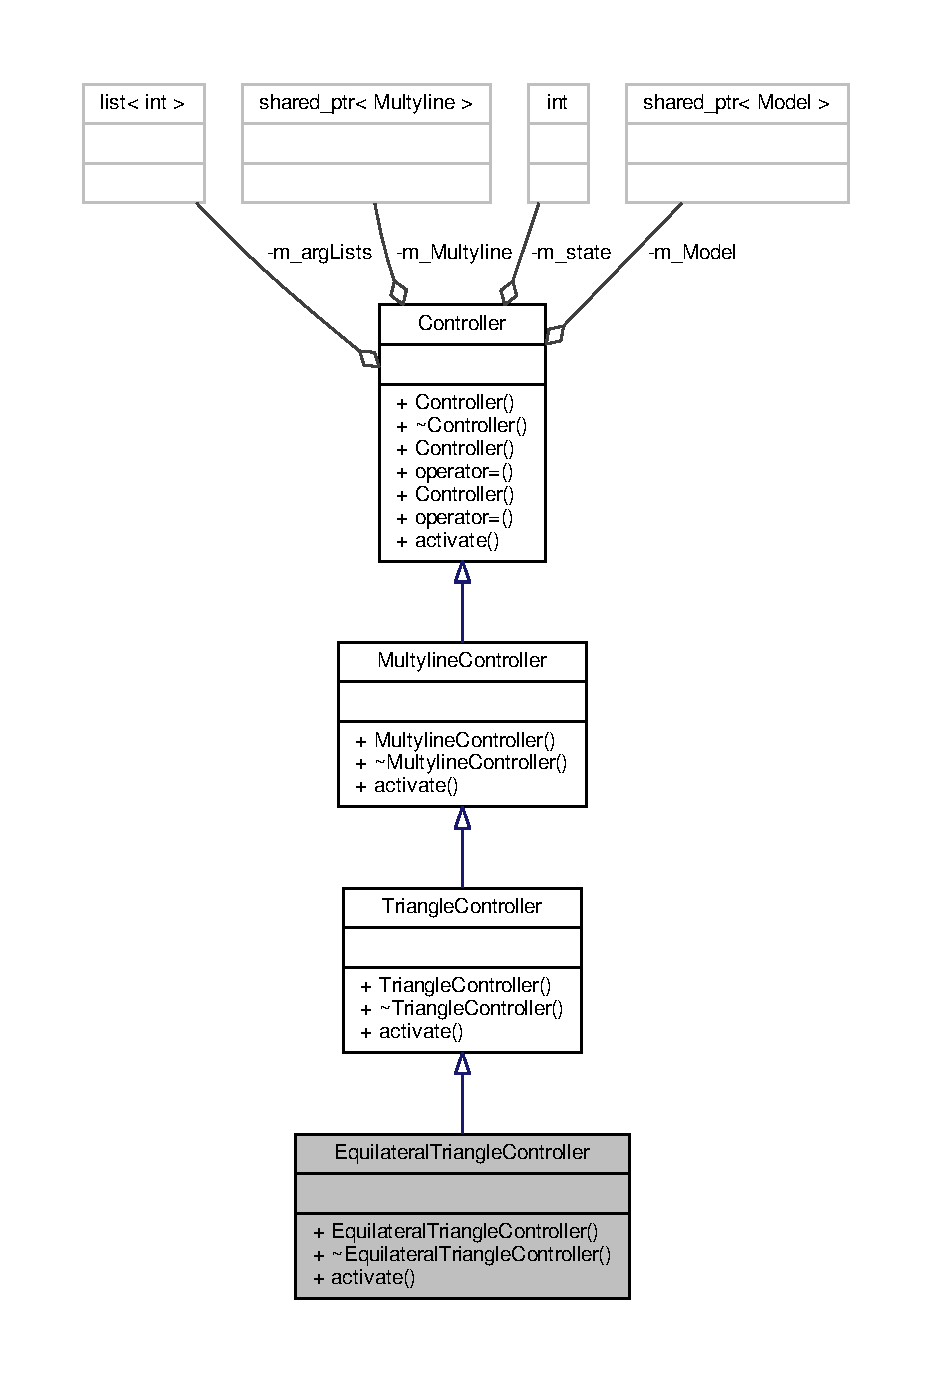
\includegraphics[width=350pt]{class_equilateral_triangle_controller__coll__graph}
\end{center}
\end{figure}
\subsection*{Открытые члены}
\begin{DoxyCompactItemize}
\item 
\hyperlink{class_equilateral_triangle_controller_a823715abcc954d05ea572f5527744e91}{Equilateral\-Triangle\-Controller} (std\-::shared\-\_\-ptr$<$ \hyperlink{class_model}{Model} $>$ \&model)
\item 
\hyperlink{class_equilateral_triangle_controller_a9cba9b68e881d99f6342f08ec3a8b64c}{$\sim$\-Equilateral\-Triangle\-Controller} ()=default
\item 
void \hyperlink{class_equilateral_triangle_controller_ac8822ad6419def097652fc8a88426898}{activate} (int cursor\-Pos\-X, int cursor\-Pos\-Y) final
\end{DoxyCompactItemize}


\subsection{Подробное описание}


См. определение в файле base\-Controller.\-h строка 157



\subsection{Конструктор(ы)}
\hypertarget{class_equilateral_triangle_controller_a823715abcc954d05ea572f5527744e91}{\index{Equilateral\-Triangle\-Controller@{Equilateral\-Triangle\-Controller}!Equilateral\-Triangle\-Controller@{Equilateral\-Triangle\-Controller}}
\index{Equilateral\-Triangle\-Controller@{Equilateral\-Triangle\-Controller}!EquilateralTriangleController@{Equilateral\-Triangle\-Controller}}
\subsubsection[{Equilateral\-Triangle\-Controller}]{\setlength{\rightskip}{0pt plus 5cm}Equilateral\-Triangle\-Controller\-::\-Equilateral\-Triangle\-Controller (
\begin{DoxyParamCaption}
\item[{std\-::shared\-\_\-ptr$<$ {\bf Model} $>$ \&}]{model}
\end{DoxyParamCaption}
)\hspace{0.3cm}{\ttfamily [inline]}}}\label{class_equilateral_triangle_controller_a823715abcc954d05ea572f5527744e91}


См. определение в файле base\-Controller.\-h строка 160

\hypertarget{class_equilateral_triangle_controller_a9cba9b68e881d99f6342f08ec3a8b64c}{\index{Equilateral\-Triangle\-Controller@{Equilateral\-Triangle\-Controller}!$\sim$\-Equilateral\-Triangle\-Controller@{$\sim$\-Equilateral\-Triangle\-Controller}}
\index{$\sim$\-Equilateral\-Triangle\-Controller@{$\sim$\-Equilateral\-Triangle\-Controller}!EquilateralTriangleController@{Equilateral\-Triangle\-Controller}}
\subsubsection[{$\sim$\-Equilateral\-Triangle\-Controller}]{\setlength{\rightskip}{0pt plus 5cm}Equilateral\-Triangle\-Controller\-::$\sim$\-Equilateral\-Triangle\-Controller (
\begin{DoxyParamCaption}
{}
\end{DoxyParamCaption}
)\hspace{0.3cm}{\ttfamily [default]}}}\label{class_equilateral_triangle_controller_a9cba9b68e881d99f6342f08ec3a8b64c}


\subsection{Методы}
\hypertarget{class_equilateral_triangle_controller_ac8822ad6419def097652fc8a88426898}{\index{Equilateral\-Triangle\-Controller@{Equilateral\-Triangle\-Controller}!activate@{activate}}
\index{activate@{activate}!EquilateralTriangleController@{Equilateral\-Triangle\-Controller}}
\subsubsection[{activate}]{\setlength{\rightskip}{0pt plus 5cm}void Equilateral\-Triangle\-Controller\-::activate (
\begin{DoxyParamCaption}
\item[{int}]{cursor\-Pos\-X, }
\item[{int}]{cursor\-Pos\-Y}
\end{DoxyParamCaption}
)\hspace{0.3cm}{\ttfamily [inline]}, {\ttfamily [final]}, {\ttfamily [virtual]}}}\label{class_equilateral_triangle_controller_ac8822ad6419def097652fc8a88426898}


Переопределяет метод предка \hyperlink{class_triangle_controller_ab86471e4de39ae99bc6198583d173c7b}{Triangle\-Controller}.



См. определение в файле base\-Controller.\-h строка 162



Объявления и описания членов класса находятся в файле\-:\begin{DoxyCompactItemize}
\item 
libs/controllers/\hyperlink{base_controller_8h}{base\-Controller.\-h}\end{DoxyCompactItemize}

\hypertarget{class_isosceles_triangle}{\section{Класс Isosceles\-Triangle}
\label{class_isosceles_triangle}\index{Isosceles\-Triangle@{Isosceles\-Triangle}}
}


{\ttfamily \#include $<$m3\-\_\-basic.\-h$>$}



Граф наследования\-:Isosceles\-Triangle\-:
\nopagebreak
\begin{figure}[H]
\begin{center}
\leavevmode
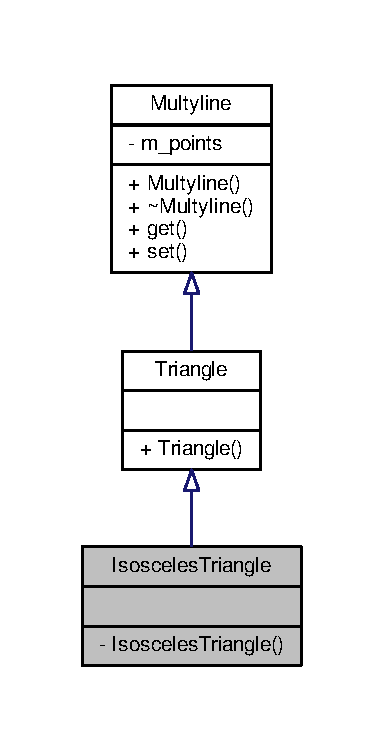
\includegraphics[width=184pt]{class_isosceles_triangle__inherit__graph}
\end{center}
\end{figure}


Граф связей класса Isosceles\-Triangle\-:
\nopagebreak
\begin{figure}[H]
\begin{center}
\leavevmode
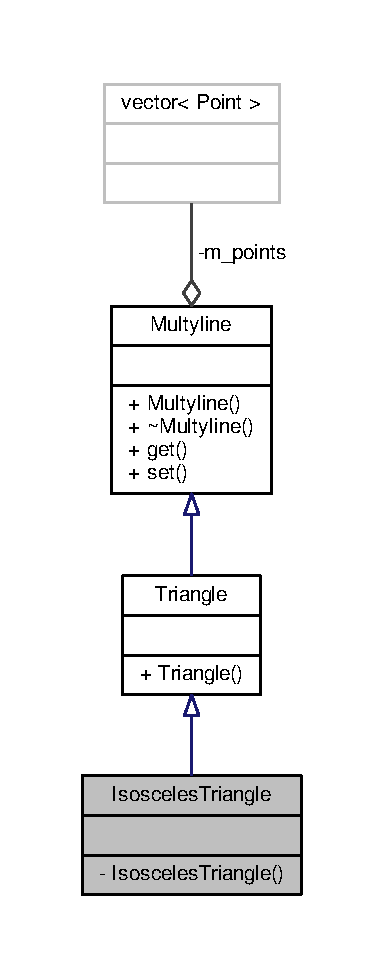
\includegraphics[width=184pt]{class_isosceles_triangle__coll__graph}
\end{center}
\end{figure}
\subsection*{Закрытые типы}
\begin{DoxyCompactItemize}
\item 
enum \hyperlink{class_isosceles_triangle_ae25b85b6ba464d8f3394eeb7b39215ff}{draw\-Method} \{ \\*
\hyperlink{class_isosceles_triangle_ae25b85b6ba464d8f3394eeb7b39215ffaff80e9fadb19575656ecfff8153263c5}{point1side}, 
\hyperlink{class_isosceles_triangle_ae25b85b6ba464d8f3394eeb7b39215ffa5a175df028aa43075ab3edfe61cd58dc}{point1base}, 
\hyperlink{class_isosceles_triangle_ae25b85b6ba464d8f3394eeb7b39215ffaca9db2a039060931ad41b18328f036a1}{point2side}, 
\hyperlink{class_isosceles_triangle_ae25b85b6ba464d8f3394eeb7b39215ffa1977a9bc1cb903b2be31a411f7fcc503}{point2base}, 
\\*
\hyperlink{class_isosceles_triangle_ae25b85b6ba464d8f3394eeb7b39215ffa24bfe64dc398220e2049528b88ddfeb2}{point3}, 
\hyperlink{class_isosceles_triangle_ae25b85b6ba464d8f3394eeb7b39215ffa56c68a99c41763d92f5f9d6a78e583a6}{mid\-Base}
 \}
\end{DoxyCompactItemize}
\subsection*{Закрытые члены}
\begin{DoxyCompactItemize}
\item 
\hyperlink{class_isosceles_triangle_a610b0c6557b9417b5ca8361b1ef4910a}{Isosceles\-Triangle} (\hyperlink{class_multyline_ad75d7bb224267d0d7b4c40fd72a1d920}{draw\-Method}, std\-::initializer\-\_\-list$<$ double $>$ \&)
\end{DoxyCompactItemize}
\subsection*{Дополнительные унаследованные члены}


\subsection{Подробное описание}


См. определение в файле m3\-\_\-basic.\-h строка 42



\subsection{Перечисления}
\hypertarget{class_isosceles_triangle_ae25b85b6ba464d8f3394eeb7b39215ff}{\index{Isosceles\-Triangle@{Isosceles\-Triangle}!draw\-Method@{draw\-Method}}
\index{draw\-Method@{draw\-Method}!IsoscelesTriangle@{Isosceles\-Triangle}}
\subsubsection[{draw\-Method}]{\setlength{\rightskip}{0pt plus 5cm}enum {\bf Isosceles\-Triangle\-::draw\-Method}\hspace{0.3cm}{\ttfamily [private]}}}\label{class_isosceles_triangle_ae25b85b6ba464d8f3394eeb7b39215ff}
\begin{Desc}
\item[Элементы перечислений]\par
\begin{description}
\index{point1side@{point1side}!Isosceles\-Triangle@{Isosceles\-Triangle}}\index{Isosceles\-Triangle@{Isosceles\-Triangle}!point1side@{point1side}}\item[{\em 
\hypertarget{class_isosceles_triangle_ae25b85b6ba464d8f3394eeb7b39215ffaff80e9fadb19575656ecfff8153263c5}{point1side}\label{class_isosceles_triangle_ae25b85b6ba464d8f3394eeb7b39215ffaff80e9fadb19575656ecfff8153263c5}
}]\index{point1base@{point1base}!Isosceles\-Triangle@{Isosceles\-Triangle}}\index{Isosceles\-Triangle@{Isosceles\-Triangle}!point1base@{point1base}}\item[{\em 
\hypertarget{class_isosceles_triangle_ae25b85b6ba464d8f3394eeb7b39215ffa5a175df028aa43075ab3edfe61cd58dc}{point1base}\label{class_isosceles_triangle_ae25b85b6ba464d8f3394eeb7b39215ffa5a175df028aa43075ab3edfe61cd58dc}
}]\index{point2side@{point2side}!Isosceles\-Triangle@{Isosceles\-Triangle}}\index{Isosceles\-Triangle@{Isosceles\-Triangle}!point2side@{point2side}}\item[{\em 
\hypertarget{class_isosceles_triangle_ae25b85b6ba464d8f3394eeb7b39215ffaca9db2a039060931ad41b18328f036a1}{point2side}\label{class_isosceles_triangle_ae25b85b6ba464d8f3394eeb7b39215ffaca9db2a039060931ad41b18328f036a1}
}]\index{point2base@{point2base}!Isosceles\-Triangle@{Isosceles\-Triangle}}\index{Isosceles\-Triangle@{Isosceles\-Triangle}!point2base@{point2base}}\item[{\em 
\hypertarget{class_isosceles_triangle_ae25b85b6ba464d8f3394eeb7b39215ffa1977a9bc1cb903b2be31a411f7fcc503}{point2base}\label{class_isosceles_triangle_ae25b85b6ba464d8f3394eeb7b39215ffa1977a9bc1cb903b2be31a411f7fcc503}
}]\index{point3@{point3}!Isosceles\-Triangle@{Isosceles\-Triangle}}\index{Isosceles\-Triangle@{Isosceles\-Triangle}!point3@{point3}}\item[{\em 
\hypertarget{class_isosceles_triangle_ae25b85b6ba464d8f3394eeb7b39215ffa24bfe64dc398220e2049528b88ddfeb2}{point3}\label{class_isosceles_triangle_ae25b85b6ba464d8f3394eeb7b39215ffa24bfe64dc398220e2049528b88ddfeb2}
}]\index{mid\-Base@{mid\-Base}!Isosceles\-Triangle@{Isosceles\-Triangle}}\index{Isosceles\-Triangle@{Isosceles\-Triangle}!mid\-Base@{mid\-Base}}\item[{\em 
\hypertarget{class_isosceles_triangle_ae25b85b6ba464d8f3394eeb7b39215ffa56c68a99c41763d92f5f9d6a78e583a6}{mid\-Base}\label{class_isosceles_triangle_ae25b85b6ba464d8f3394eeb7b39215ffa56c68a99c41763d92f5f9d6a78e583a6}
}]\end{description}
\end{Desc}


См. определение в файле m3\-\_\-basic.\-h строка 44



\subsection{Конструктор(ы)}
\hypertarget{class_isosceles_triangle_a610b0c6557b9417b5ca8361b1ef4910a}{\index{Isosceles\-Triangle@{Isosceles\-Triangle}!Isosceles\-Triangle@{Isosceles\-Triangle}}
\index{Isosceles\-Triangle@{Isosceles\-Triangle}!IsoscelesTriangle@{Isosceles\-Triangle}}
\subsubsection[{Isosceles\-Triangle}]{\setlength{\rightskip}{0pt plus 5cm}Isosceles\-Triangle\-::\-Isosceles\-Triangle (
\begin{DoxyParamCaption}
\item[{{\bf draw\-Method}}]{, }
\item[{std\-::initializer\-\_\-list$<$ double $>$ \&}]{}
\end{DoxyParamCaption}
)\hspace{0.3cm}{\ttfamily [private]}}}\label{class_isosceles_triangle_a610b0c6557b9417b5ca8361b1ef4910a}


Объявления и описания членов класса находятся в файле\-:\begin{DoxyCompactItemize}
\item 
libs/models/m\-\_\-shapes/\hyperlink{m3__basic_8h}{m3\-\_\-basic.\-h}\end{DoxyCompactItemize}

\hypertarget{class_isosceles_triangle_controller}{\section{Класс Isosceles\-Triangle\-Controller}
\label{class_isosceles_triangle_controller}\index{Isosceles\-Triangle\-Controller@{Isosceles\-Triangle\-Controller}}
}


{\ttfamily \#include $<$base\-Controller.\-h$>$}



Граф наследования\-:Isosceles\-Triangle\-Controller\-:
\nopagebreak
\begin{figure}[H]
\begin{center}
\leavevmode
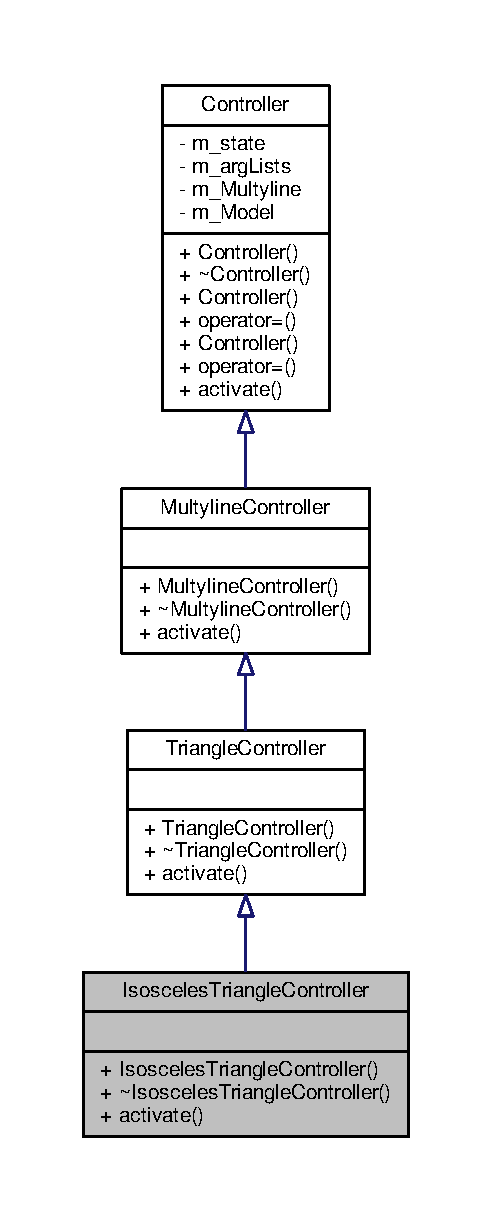
\includegraphics[height=550pt]{class_isosceles_triangle_controller__inherit__graph}
\end{center}
\end{figure}


Граф связей класса Isosceles\-Triangle\-Controller\-:
\nopagebreak
\begin{figure}[H]
\begin{center}
\leavevmode
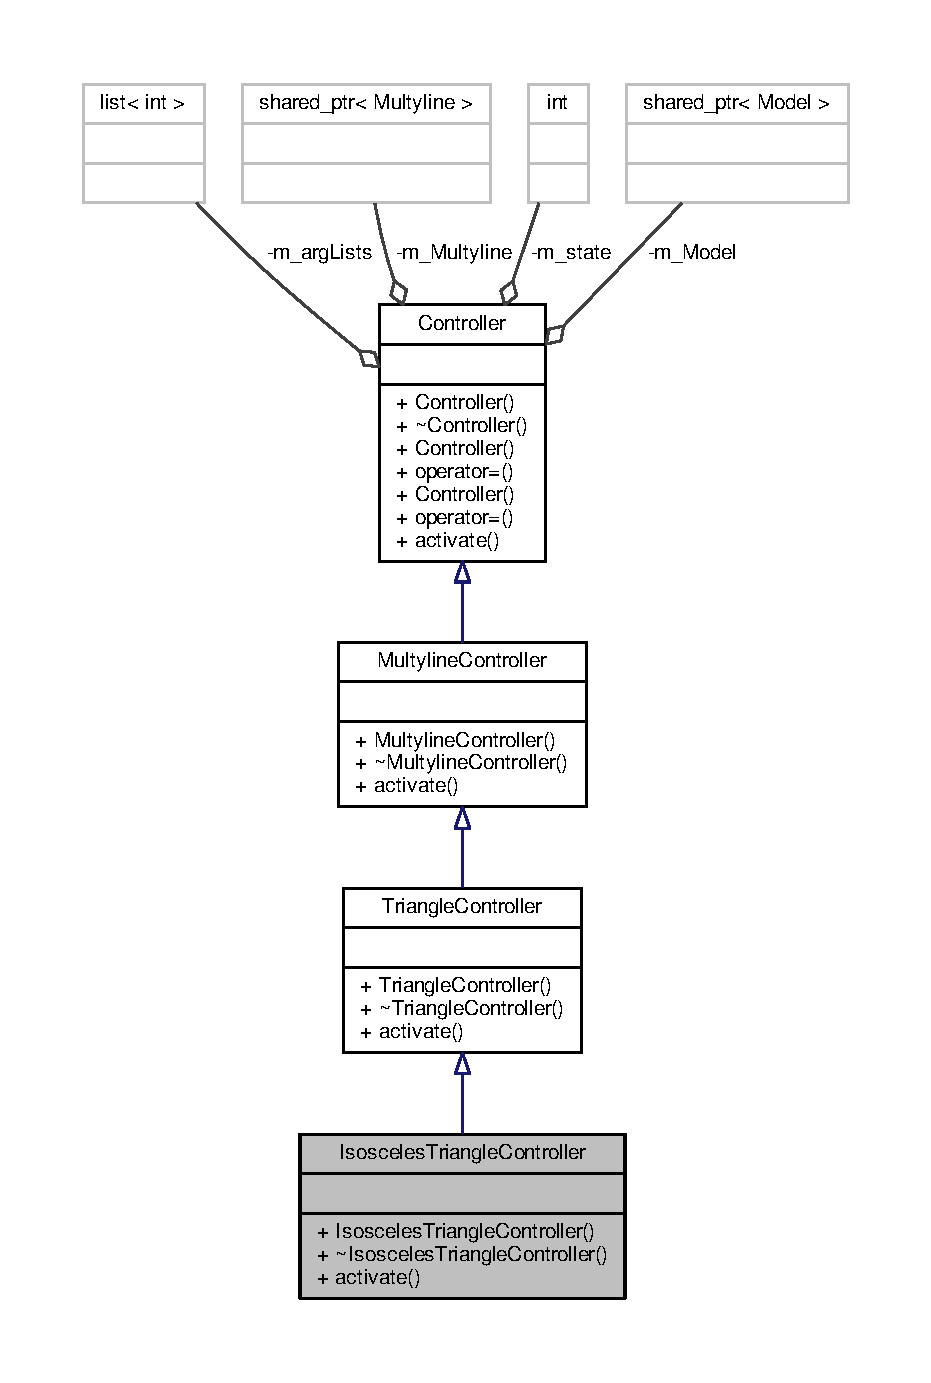
\includegraphics[width=350pt]{class_isosceles_triangle_controller__coll__graph}
\end{center}
\end{figure}
\subsection*{Открытые члены}
\begin{DoxyCompactItemize}
\item 
\hyperlink{class_isosceles_triangle_controller_ad8bf1a8c726e6b4279be064a4875062e}{Isosceles\-Triangle\-Controller} (std\-::shared\-\_\-ptr$<$ \hyperlink{class_model}{Model} $>$ \&model)
\item 
\hyperlink{class_isosceles_triangle_controller_a54ec5774792ce310505e4d3ea48d3ce9}{$\sim$\-Isosceles\-Triangle\-Controller} ()=default
\item 
void \hyperlink{class_isosceles_triangle_controller_ac060b7bdfdc3c5fc078147e14e31415b}{activate} (int cursor\-Pos\-X, int cursor\-Pos\-Y) final
\end{DoxyCompactItemize}


\subsection{Подробное описание}


См. определение в файле base\-Controller.\-h строка 144



\subsection{Конструктор(ы)}
\hypertarget{class_isosceles_triangle_controller_ad8bf1a8c726e6b4279be064a4875062e}{\index{Isosceles\-Triangle\-Controller@{Isosceles\-Triangle\-Controller}!Isosceles\-Triangle\-Controller@{Isosceles\-Triangle\-Controller}}
\index{Isosceles\-Triangle\-Controller@{Isosceles\-Triangle\-Controller}!IsoscelesTriangleController@{Isosceles\-Triangle\-Controller}}
\subsubsection[{Isosceles\-Triangle\-Controller}]{\setlength{\rightskip}{0pt plus 5cm}Isosceles\-Triangle\-Controller\-::\-Isosceles\-Triangle\-Controller (
\begin{DoxyParamCaption}
\item[{std\-::shared\-\_\-ptr$<$ {\bf Model} $>$ \&}]{model}
\end{DoxyParamCaption}
)\hspace{0.3cm}{\ttfamily [inline]}}}\label{class_isosceles_triangle_controller_ad8bf1a8c726e6b4279be064a4875062e}


См. определение в файле base\-Controller.\-h строка 147

\hypertarget{class_isosceles_triangle_controller_a54ec5774792ce310505e4d3ea48d3ce9}{\index{Isosceles\-Triangle\-Controller@{Isosceles\-Triangle\-Controller}!$\sim$\-Isosceles\-Triangle\-Controller@{$\sim$\-Isosceles\-Triangle\-Controller}}
\index{$\sim$\-Isosceles\-Triangle\-Controller@{$\sim$\-Isosceles\-Triangle\-Controller}!IsoscelesTriangleController@{Isosceles\-Triangle\-Controller}}
\subsubsection[{$\sim$\-Isosceles\-Triangle\-Controller}]{\setlength{\rightskip}{0pt plus 5cm}Isosceles\-Triangle\-Controller\-::$\sim$\-Isosceles\-Triangle\-Controller (
\begin{DoxyParamCaption}
{}
\end{DoxyParamCaption}
)\hspace{0.3cm}{\ttfamily [default]}}}\label{class_isosceles_triangle_controller_a54ec5774792ce310505e4d3ea48d3ce9}


\subsection{Методы}
\hypertarget{class_isosceles_triangle_controller_ac060b7bdfdc3c5fc078147e14e31415b}{\index{Isosceles\-Triangle\-Controller@{Isosceles\-Triangle\-Controller}!activate@{activate}}
\index{activate@{activate}!IsoscelesTriangleController@{Isosceles\-Triangle\-Controller}}
\subsubsection[{activate}]{\setlength{\rightskip}{0pt plus 5cm}void Isosceles\-Triangle\-Controller\-::activate (
\begin{DoxyParamCaption}
\item[{int}]{cursor\-Pos\-X, }
\item[{int}]{cursor\-Pos\-Y}
\end{DoxyParamCaption}
)\hspace{0.3cm}{\ttfamily [inline]}, {\ttfamily [final]}, {\ttfamily [virtual]}}}\label{class_isosceles_triangle_controller_ac060b7bdfdc3c5fc078147e14e31415b}


Переопределяет метод предка \hyperlink{class_triangle_controller_ab86471e4de39ae99bc6198583d173c7b}{Triangle\-Controller}.



См. определение в файле base\-Controller.\-h строка 149



Объявления и описания членов класса находятся в файле\-:\begin{DoxyCompactItemize}
\item 
libs/controllers/\hyperlink{base_controller_8h}{base\-Controller.\-h}\end{DoxyCompactItemize}

\hypertarget{class_load_controller}{\section{Класс Load\-Controller}
\label{class_load_controller}\index{Load\-Controller@{Load\-Controller}}
}


{\ttfamily \#include $<$base\-Controller.\-h$>$}



Граф наследования\-:Load\-Controller\-:
\nopagebreak
\begin{figure}[H]
\begin{center}
\leavevmode
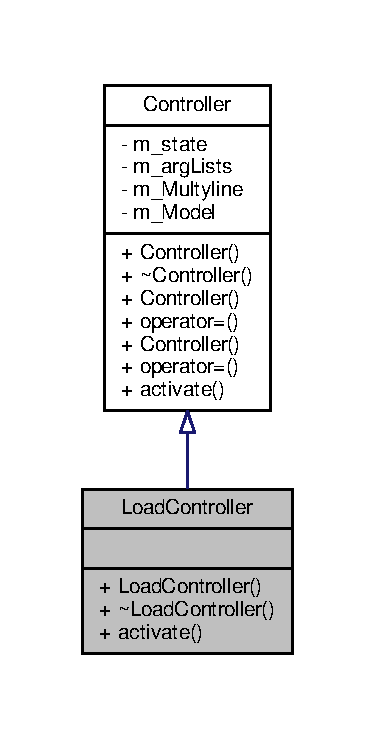
\includegraphics[width=180pt]{class_load_controller__inherit__graph}
\end{center}
\end{figure}


Граф связей класса Load\-Controller\-:
\nopagebreak
\begin{figure}[H]
\begin{center}
\leavevmode
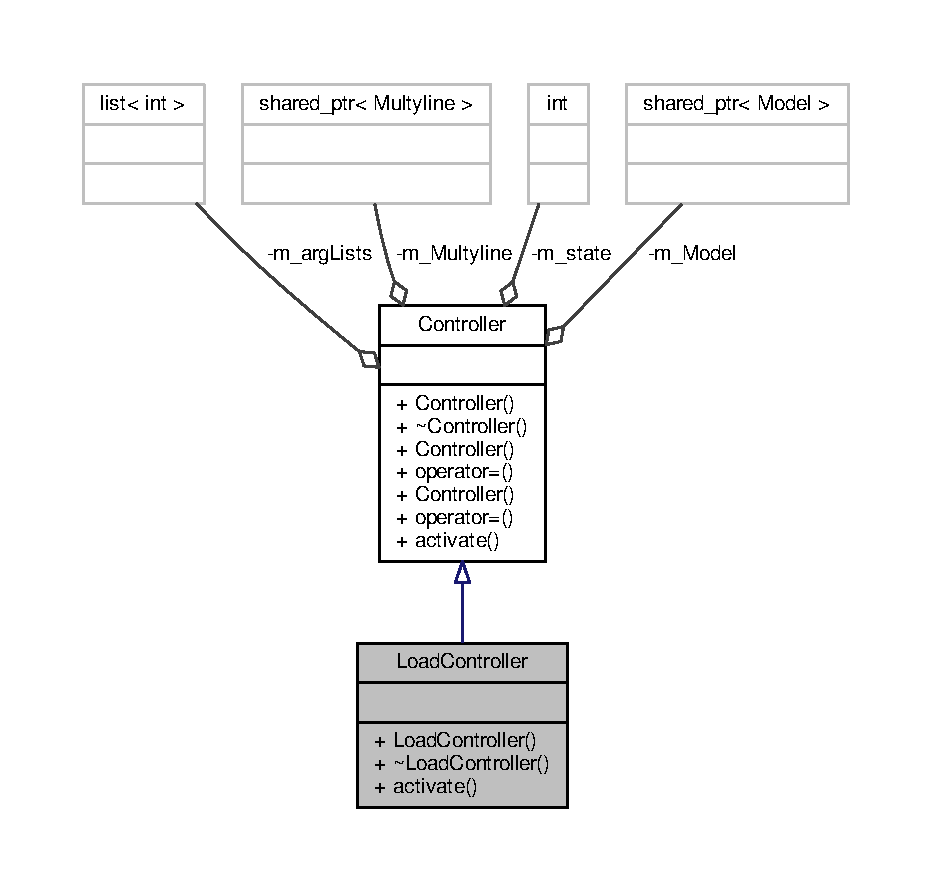
\includegraphics[width=350pt]{class_load_controller__coll__graph}
\end{center}
\end{figure}
\subsection*{Открытые члены}
\begin{DoxyCompactItemize}
\item 
\hyperlink{class_load_controller_acb89a633078f6fd64c60c98c9ead4c49}{Load\-Controller} (std\-::shared\-\_\-ptr$<$ \hyperlink{class_model}{Model} $>$ \&model)
\item 
\hyperlink{class_load_controller_ab4d73ee743830dd22bcc0857656f77f7}{$\sim$\-Load\-Controller} ()=default
\item 
void \hyperlink{class_load_controller_aa9fc9b866ea0abda7d8d766ffa9256f4}{activate} (int cursor\-Pos\-X, int cursor\-Pos\-Y) final
\end{DoxyCompactItemize}


\subsection{Подробное описание}


См. определение в файле base\-Controller.\-h строка 48



\subsection{Конструктор(ы)}
\hypertarget{class_load_controller_acb89a633078f6fd64c60c98c9ead4c49}{\index{Load\-Controller@{Load\-Controller}!Load\-Controller@{Load\-Controller}}
\index{Load\-Controller@{Load\-Controller}!LoadController@{Load\-Controller}}
\subsubsection[{Load\-Controller}]{\setlength{\rightskip}{0pt plus 5cm}Load\-Controller\-::\-Load\-Controller (
\begin{DoxyParamCaption}
\item[{std\-::shared\-\_\-ptr$<$ {\bf Model} $>$ \&}]{model}
\end{DoxyParamCaption}
)\hspace{0.3cm}{\ttfamily [inline]}}}\label{class_load_controller_acb89a633078f6fd64c60c98c9ead4c49}


См. определение в файле base\-Controller.\-h строка 51

\hypertarget{class_load_controller_ab4d73ee743830dd22bcc0857656f77f7}{\index{Load\-Controller@{Load\-Controller}!$\sim$\-Load\-Controller@{$\sim$\-Load\-Controller}}
\index{$\sim$\-Load\-Controller@{$\sim$\-Load\-Controller}!LoadController@{Load\-Controller}}
\subsubsection[{$\sim$\-Load\-Controller}]{\setlength{\rightskip}{0pt plus 5cm}Load\-Controller\-::$\sim$\-Load\-Controller (
\begin{DoxyParamCaption}
{}
\end{DoxyParamCaption}
)\hspace{0.3cm}{\ttfamily [default]}}}\label{class_load_controller_ab4d73ee743830dd22bcc0857656f77f7}


\subsection{Методы}
\hypertarget{class_load_controller_aa9fc9b866ea0abda7d8d766ffa9256f4}{\index{Load\-Controller@{Load\-Controller}!activate@{activate}}
\index{activate@{activate}!LoadController@{Load\-Controller}}
\subsubsection[{activate}]{\setlength{\rightskip}{0pt plus 5cm}void Load\-Controller\-::activate (
\begin{DoxyParamCaption}
\item[{int}]{cursor\-Pos\-X, }
\item[{int}]{cursor\-Pos\-Y}
\end{DoxyParamCaption}
)\hspace{0.3cm}{\ttfamily [inline]}, {\ttfamily [final]}, {\ttfamily [virtual]}}}\label{class_load_controller_aa9fc9b866ea0abda7d8d766ffa9256f4}


Замещает \hyperlink{class_controller_a4cc69a630011f49efb0c221d617af633}{Controller}.



См. определение в файле base\-Controller.\-h строка 53



Объявления и описания членов класса находятся в файле\-:\begin{DoxyCompactItemize}
\item 
libs/controllers/\hyperlink{base_controller_8h}{base\-Controller.\-h}\end{DoxyCompactItemize}

\hypertarget{class_main_controller}{\section{Класс Main\-Controller}
\label{class_main_controller}\index{Main\-Controller@{Main\-Controller}}
}


{\ttfamily \#include $<$controller.\-h$>$}



Граф связей класса Main\-Controller\-:
\nopagebreak
\begin{figure}[H]
\begin{center}
\leavevmode
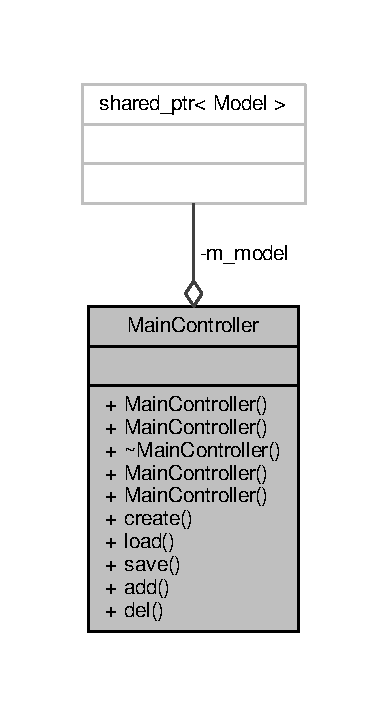
\includegraphics[width=186pt]{class_main_controller__coll__graph}
\end{center}
\end{figure}
\subsection*{Открытые члены}
\begin{DoxyCompactItemize}
\item 
\hyperlink{class_main_controller_ab04905d2ca29c6375c6cde8201327b06}{Main\-Controller} ()=default
\item 
\hyperlink{class_main_controller_a457b718690b3c2101b00ea2295d5c4b3}{Main\-Controller} (\hyperlink{class_model}{Model} \&\-\_\-model)
\item 
\hyperlink{class_main_controller_aa7e960df99b2c9f24abc52d7863c7fa1}{$\sim$\-Main\-Controller} ()=default
\item 
\hyperlink{class_main_controller_aedd8d4a7b9cb71ab9b95912d0786a4e3}{Main\-Controller} (const \hyperlink{class_main_controller}{Main\-Controller} \&)=default
\item 
\hyperlink{class_main_controller_af1951b682e657fd7e43d354159984a3f}{Main\-Controller} (\hyperlink{class_main_controller}{Main\-Controller} \&\&)=default
\item 
void \hyperlink{class_main_controller_a4875e8ce5645793e06377d758cfba6ef}{create} ()
\item 
void \hyperlink{class_main_controller_a3dedc9e9860fb2e153310d7372038c0d}{load} ()
\item 
void \hyperlink{class_main_controller_a06797caf7960caaa8276b30ee488eb1d}{save} ()
\item 
void \hyperlink{class_main_controller_a56fa760f0bbc517c14b770fac94d0fe1}{add} (const \hyperlink{class_multyline}{Multyline} \&)
\item 
void \hyperlink{class_main_controller_a83908eb37bff0af06054fb8ef5de017d}{del} (const \hyperlink{class_multyline}{Multyline} \&)
\end{DoxyCompactItemize}
\subsection*{Закрытые данные}
\begin{DoxyCompactItemize}
\item 
std\-::shared\-\_\-ptr$<$ \hyperlink{class_model}{Model} $>$ \hyperlink{class_main_controller_aec52515a794e452bbf6ccf186d96cc53}{m\-\_\-model}
\end{DoxyCompactItemize}


\subsection{Подробное описание}


См. определение в файле controller.\-h строка 8



\subsection{Конструктор(ы)}
\hypertarget{class_main_controller_ab04905d2ca29c6375c6cde8201327b06}{\index{Main\-Controller@{Main\-Controller}!Main\-Controller@{Main\-Controller}}
\index{Main\-Controller@{Main\-Controller}!MainController@{Main\-Controller}}
\subsubsection[{Main\-Controller}]{\setlength{\rightskip}{0pt plus 5cm}Main\-Controller\-::\-Main\-Controller (
\begin{DoxyParamCaption}
{}
\end{DoxyParamCaption}
)\hspace{0.3cm}{\ttfamily [default]}}}\label{class_main_controller_ab04905d2ca29c6375c6cde8201327b06}
\hypertarget{class_main_controller_a457b718690b3c2101b00ea2295d5c4b3}{\index{Main\-Controller@{Main\-Controller}!Main\-Controller@{Main\-Controller}}
\index{Main\-Controller@{Main\-Controller}!MainController@{Main\-Controller}}
\subsubsection[{Main\-Controller}]{\setlength{\rightskip}{0pt plus 5cm}Main\-Controller\-::\-Main\-Controller (
\begin{DoxyParamCaption}
\item[{{\bf Model} \&}]{\-\_\-model}
\end{DoxyParamCaption}
)\hspace{0.3cm}{\ttfamily [inline]}}}\label{class_main_controller_a457b718690b3c2101b00ea2295d5c4b3}


См. определение в файле controller.\-h строка 12

\hypertarget{class_main_controller_aa7e960df99b2c9f24abc52d7863c7fa1}{\index{Main\-Controller@{Main\-Controller}!$\sim$\-Main\-Controller@{$\sim$\-Main\-Controller}}
\index{$\sim$\-Main\-Controller@{$\sim$\-Main\-Controller}!MainController@{Main\-Controller}}
\subsubsection[{$\sim$\-Main\-Controller}]{\setlength{\rightskip}{0pt plus 5cm}Main\-Controller\-::$\sim$\-Main\-Controller (
\begin{DoxyParamCaption}
{}
\end{DoxyParamCaption}
)\hspace{0.3cm}{\ttfamily [default]}}}\label{class_main_controller_aa7e960df99b2c9f24abc52d7863c7fa1}
\hypertarget{class_main_controller_aedd8d4a7b9cb71ab9b95912d0786a4e3}{\index{Main\-Controller@{Main\-Controller}!Main\-Controller@{Main\-Controller}}
\index{Main\-Controller@{Main\-Controller}!MainController@{Main\-Controller}}
\subsubsection[{Main\-Controller}]{\setlength{\rightskip}{0pt plus 5cm}Main\-Controller\-::\-Main\-Controller (
\begin{DoxyParamCaption}
\item[{const {\bf Main\-Controller} \&}]{}
\end{DoxyParamCaption}
)\hspace{0.3cm}{\ttfamily [default]}}}\label{class_main_controller_aedd8d4a7b9cb71ab9b95912d0786a4e3}
\hypertarget{class_main_controller_af1951b682e657fd7e43d354159984a3f}{\index{Main\-Controller@{Main\-Controller}!Main\-Controller@{Main\-Controller}}
\index{Main\-Controller@{Main\-Controller}!MainController@{Main\-Controller}}
\subsubsection[{Main\-Controller}]{\setlength{\rightskip}{0pt plus 5cm}Main\-Controller\-::\-Main\-Controller (
\begin{DoxyParamCaption}
\item[{{\bf Main\-Controller} \&\&}]{}
\end{DoxyParamCaption}
)\hspace{0.3cm}{\ttfamily [default]}}}\label{class_main_controller_af1951b682e657fd7e43d354159984a3f}


\subsection{Методы}
\hypertarget{class_main_controller_a56fa760f0bbc517c14b770fac94d0fe1}{\index{Main\-Controller@{Main\-Controller}!add@{add}}
\index{add@{add}!MainController@{Main\-Controller}}
\subsubsection[{add}]{\setlength{\rightskip}{0pt plus 5cm}void Main\-Controller\-::add (
\begin{DoxyParamCaption}
\item[{const {\bf Multyline} \&}]{}
\end{DoxyParamCaption}
)}}\label{class_main_controller_a56fa760f0bbc517c14b770fac94d0fe1}
\hypertarget{class_main_controller_a4875e8ce5645793e06377d758cfba6ef}{\index{Main\-Controller@{Main\-Controller}!create@{create}}
\index{create@{create}!MainController@{Main\-Controller}}
\subsubsection[{create}]{\setlength{\rightskip}{0pt plus 5cm}void Main\-Controller\-::create (
\begin{DoxyParamCaption}
{}
\end{DoxyParamCaption}
)}}\label{class_main_controller_a4875e8ce5645793e06377d758cfba6ef}
\hypertarget{class_main_controller_a83908eb37bff0af06054fb8ef5de017d}{\index{Main\-Controller@{Main\-Controller}!del@{del}}
\index{del@{del}!MainController@{Main\-Controller}}
\subsubsection[{del}]{\setlength{\rightskip}{0pt plus 5cm}void Main\-Controller\-::del (
\begin{DoxyParamCaption}
\item[{const {\bf Multyline} \&}]{}
\end{DoxyParamCaption}
)}}\label{class_main_controller_a83908eb37bff0af06054fb8ef5de017d}
\hypertarget{class_main_controller_a3dedc9e9860fb2e153310d7372038c0d}{\index{Main\-Controller@{Main\-Controller}!load@{load}}
\index{load@{load}!MainController@{Main\-Controller}}
\subsubsection[{load}]{\setlength{\rightskip}{0pt plus 5cm}void Main\-Controller\-::load (
\begin{DoxyParamCaption}
{}
\end{DoxyParamCaption}
)}}\label{class_main_controller_a3dedc9e9860fb2e153310d7372038c0d}
\hypertarget{class_main_controller_a06797caf7960caaa8276b30ee488eb1d}{\index{Main\-Controller@{Main\-Controller}!save@{save}}
\index{save@{save}!MainController@{Main\-Controller}}
\subsubsection[{save}]{\setlength{\rightskip}{0pt plus 5cm}void Main\-Controller\-::save (
\begin{DoxyParamCaption}
{}
\end{DoxyParamCaption}
)}}\label{class_main_controller_a06797caf7960caaa8276b30ee488eb1d}


\subsection{Данные класса}
\hypertarget{class_main_controller_aec52515a794e452bbf6ccf186d96cc53}{\index{Main\-Controller@{Main\-Controller}!m\-\_\-model@{m\-\_\-model}}
\index{m\-\_\-model@{m\-\_\-model}!MainController@{Main\-Controller}}
\subsubsection[{m\-\_\-model}]{\setlength{\rightskip}{0pt plus 5cm}std\-::shared\-\_\-ptr$<${\bf Model}$>$ Main\-Controller\-::m\-\_\-model\hspace{0.3cm}{\ttfamily [private]}}}\label{class_main_controller_aec52515a794e452bbf6ccf186d96cc53}


См. определение в файле controller.\-h строка 51



Объявления и описания членов класса находятся в файле\-:\begin{DoxyCompactItemize}
\item 
libs/\hyperlink{controller_8h}{controller.\-h}\end{DoxyCompactItemize}

\hypertarget{class_model}{\section{Класс Model}
\label{class_model}\index{Model@{Model}}
}


{\ttfamily \#include $<$model.\-h$>$}



Граф связей класса Model\-:
\nopagebreak
\begin{figure}[H]
\begin{center}
\leavevmode
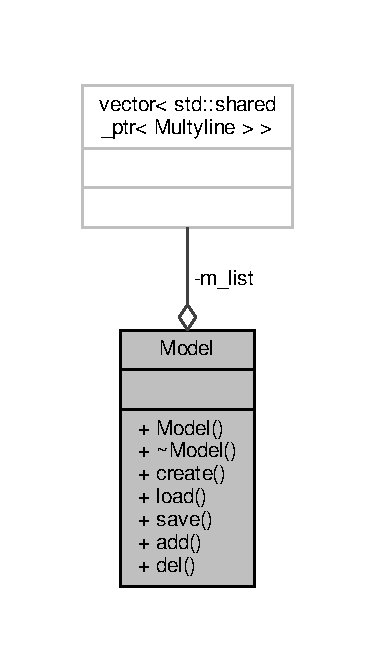
\includegraphics[width=180pt]{class_model__coll__graph}
\end{center}
\end{figure}
\subsection*{Открытые члены}
\begin{DoxyCompactItemize}
\item 
\hyperlink{class_model_ae3b375de5f6df4faf74a95d64748e048}{Model} ()
\item 
\hyperlink{class_model_ad6ebd2062a0b823db841a0b88baac4c0}{$\sim$\-Model} ()
\item 
void \hyperlink{class_model_af83f7bf343a69dd3d09131d9d2b2abe9}{create} ()
\item 
void \hyperlink{class_model_a937f7f22c88f8c6ca549b7bb98190563}{load} ()
\item 
void \hyperlink{class_model_aef4314ff5eaadebafafb9ad6dcafe5e3}{save} ()
\item 
void \hyperlink{class_model_a1cf26e1d5b881d90f91f6ae50a3c3d11}{add} (const \hyperlink{class_multyline}{Multyline} \&)
\item 
void \hyperlink{class_model_a41130e2e14fa6299db1fcf7437347eed}{del} (const \hyperlink{class_multyline}{Multyline} \&)
\end{DoxyCompactItemize}
\subsection*{Закрытые данные}
\begin{DoxyCompactItemize}
\item 
std\-::vector$<$ std\-::shared\-\_\-ptr\\*
$<$ \hyperlink{class_multyline}{Multyline} $>$ $>$ \hyperlink{class_model_a8c74aeab20b2e33ba2bc7a6d20e4afe4}{m\-\_\-list}
\end{DoxyCompactItemize}


\subsection{Подробное описание}


См. определение в файле model.\-h строка 14



\subsection{Конструктор(ы)}
\hypertarget{class_model_ae3b375de5f6df4faf74a95d64748e048}{\index{Model@{Model}!Model@{Model}}
\index{Model@{Model}!Model@{Model}}
\subsubsection[{Model}]{\setlength{\rightskip}{0pt plus 5cm}Model\-::\-Model (
\begin{DoxyParamCaption}
{}
\end{DoxyParamCaption}
)\hspace{0.3cm}{\ttfamily [inline]}}}\label{class_model_ae3b375de5f6df4faf74a95d64748e048}


См. определение в файле model.\-h строка 17

\hypertarget{class_model_ad6ebd2062a0b823db841a0b88baac4c0}{\index{Model@{Model}!$\sim$\-Model@{$\sim$\-Model}}
\index{$\sim$\-Model@{$\sim$\-Model}!Model@{Model}}
\subsubsection[{$\sim$\-Model}]{\setlength{\rightskip}{0pt plus 5cm}Model\-::$\sim$\-Model (
\begin{DoxyParamCaption}
{}
\end{DoxyParamCaption}
)\hspace{0.3cm}{\ttfamily [inline]}}}\label{class_model_ad6ebd2062a0b823db841a0b88baac4c0}


См. определение в файле model.\-h строка 18



\subsection{Методы}
\hypertarget{class_model_a1cf26e1d5b881d90f91f6ae50a3c3d11}{\index{Model@{Model}!add@{add}}
\index{add@{add}!Model@{Model}}
\subsubsection[{add}]{\setlength{\rightskip}{0pt plus 5cm}void Model\-::add (
\begin{DoxyParamCaption}
\item[{const {\bf Multyline} \&}]{}
\end{DoxyParamCaption}
)}}\label{class_model_a1cf26e1d5b881d90f91f6ae50a3c3d11}


См. определение в файле model.\-cpp строка 13

\hypertarget{class_model_af83f7bf343a69dd3d09131d9d2b2abe9}{\index{Model@{Model}!create@{create}}
\index{create@{create}!Model@{Model}}
\subsubsection[{create}]{\setlength{\rightskip}{0pt plus 5cm}void Model\-::create (
\begin{DoxyParamCaption}
{}
\end{DoxyParamCaption}
)}}\label{class_model_af83f7bf343a69dd3d09131d9d2b2abe9}


См. определение в файле model.\-cpp строка 7

\hypertarget{class_model_a41130e2e14fa6299db1fcf7437347eed}{\index{Model@{Model}!del@{del}}
\index{del@{del}!Model@{Model}}
\subsubsection[{del}]{\setlength{\rightskip}{0pt plus 5cm}void Model\-::del (
\begin{DoxyParamCaption}
\item[{const {\bf Multyline} \&}]{}
\end{DoxyParamCaption}
)}}\label{class_model_a41130e2e14fa6299db1fcf7437347eed}


См. определение в файле model.\-cpp строка 15

\hypertarget{class_model_a937f7f22c88f8c6ca549b7bb98190563}{\index{Model@{Model}!load@{load}}
\index{load@{load}!Model@{Model}}
\subsubsection[{load}]{\setlength{\rightskip}{0pt plus 5cm}void Model\-::load (
\begin{DoxyParamCaption}
{}
\end{DoxyParamCaption}
)}}\label{class_model_a937f7f22c88f8c6ca549b7bb98190563}


См. определение в файле model.\-cpp строка 9

\hypertarget{class_model_aef4314ff5eaadebafafb9ad6dcafe5e3}{\index{Model@{Model}!save@{save}}
\index{save@{save}!Model@{Model}}
\subsubsection[{save}]{\setlength{\rightskip}{0pt plus 5cm}void Model\-::save (
\begin{DoxyParamCaption}
{}
\end{DoxyParamCaption}
)}}\label{class_model_aef4314ff5eaadebafafb9ad6dcafe5e3}


См. определение в файле model.\-cpp строка 11



\subsection{Данные класса}
\hypertarget{class_model_a8c74aeab20b2e33ba2bc7a6d20e4afe4}{\index{Model@{Model}!m\-\_\-list@{m\-\_\-list}}
\index{m\-\_\-list@{m\-\_\-list}!Model@{Model}}
\subsubsection[{m\-\_\-list}]{\setlength{\rightskip}{0pt plus 5cm}std\-::vector$<$std\-::shared\-\_\-ptr$<${\bf Multyline}$>$ $>$ Model\-::m\-\_\-list\hspace{0.3cm}{\ttfamily [private]}}}\label{class_model_a8c74aeab20b2e33ba2bc7a6d20e4afe4}


См. определение в файле model.\-h строка 54



Объявления и описания членов классов находятся в файлах\-:\begin{DoxyCompactItemize}
\item 
libs/\hyperlink{model_8h}{model.\-h}\item 
libs/\hyperlink{model_8cpp}{model.\-cpp}\end{DoxyCompactItemize}

\hypertarget{class_multyline}{\section{Класс Multyline}
\label{class_multyline}\index{Multyline@{Multyline}}
}


{\ttfamily \#include $<$m\-\_\-multyline.\-h$>$}



Граф наследования\-:Multyline\-:
\nopagebreak
\begin{figure}[H]
\begin{center}
\leavevmode
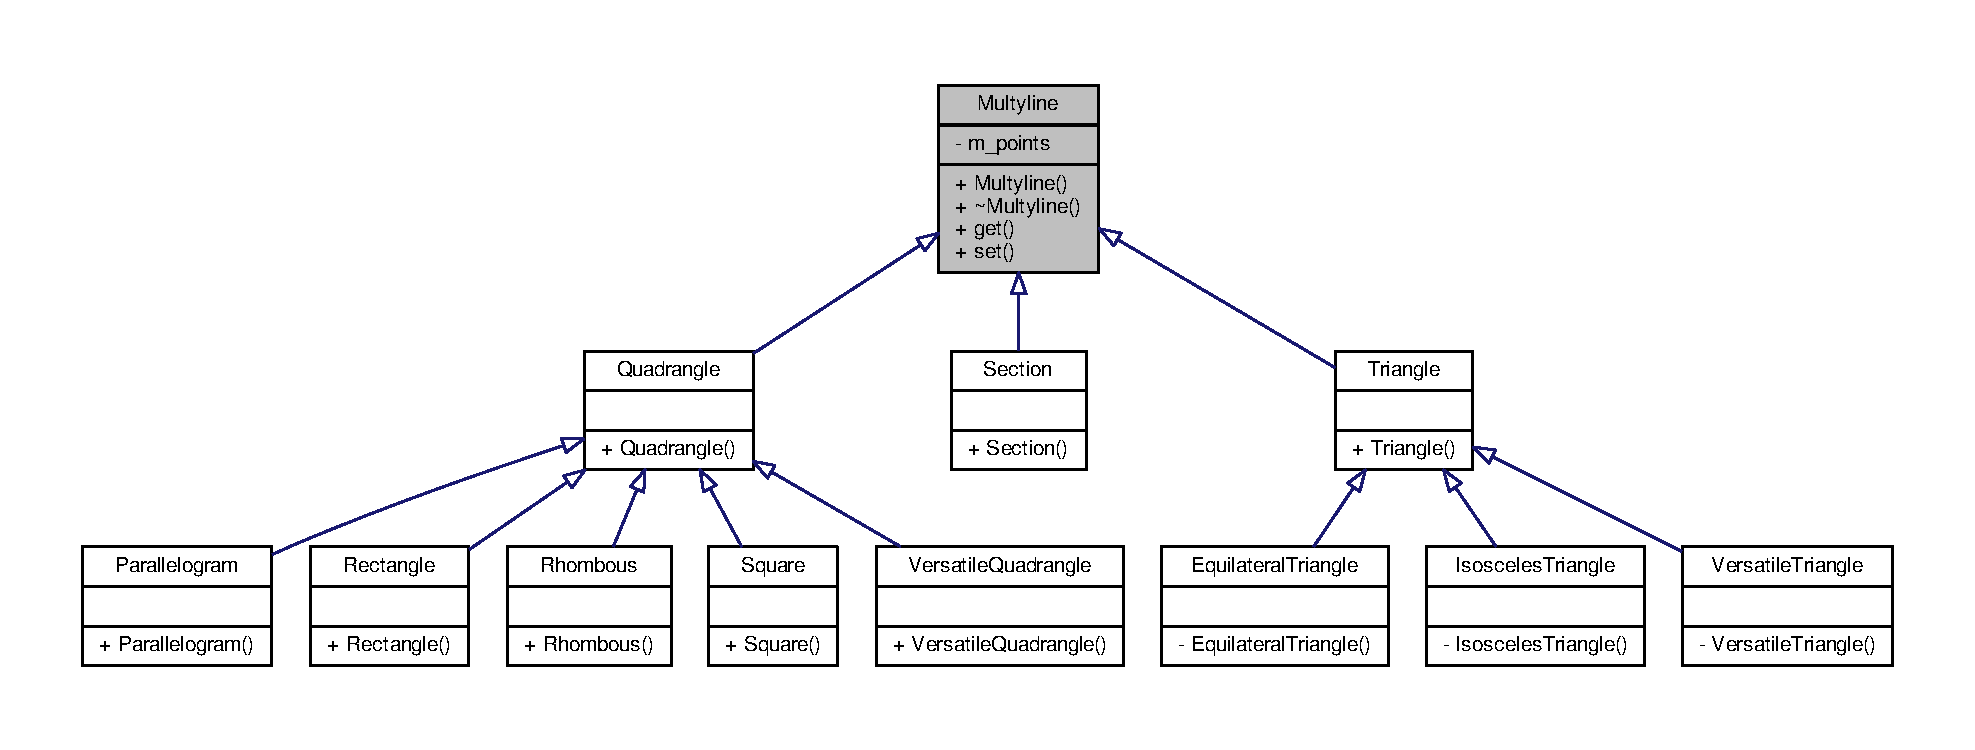
\includegraphics[width=350pt]{class_multyline__inherit__graph}
\end{center}
\end{figure}


Граф связей класса Multyline\-:
\nopagebreak
\begin{figure}[H]
\begin{center}
\leavevmode
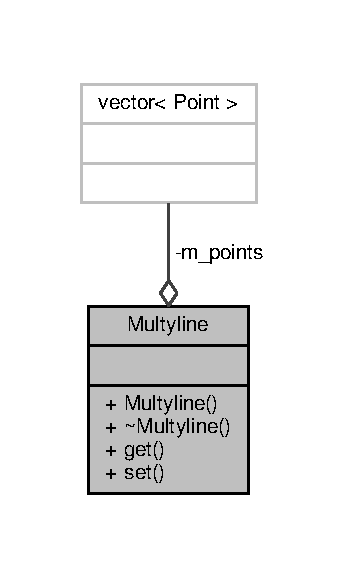
\includegraphics[width=167pt]{class_multyline__coll__graph}
\end{center}
\end{figure}
\subsection*{Открытые типы}
\begin{DoxyCompactItemize}
\item 
enum \hyperlink{class_multyline_ad75d7bb224267d0d7b4c40fd72a1d920}{draw\-Method} 
\end{DoxyCompactItemize}
\subsection*{Открытые члены}
\begin{DoxyCompactItemize}
\item 
\hyperlink{class_multyline_a36da9060517bf786ffd282587de95a12}{Multyline} (std\-::initializer\-\_\-list$<$ double $>$)
\item 
virtual \hyperlink{class_multyline_ae4a567046d3708fe823a9990b9925845}{$\sim$\-Multyline} ()
\item 
const \hyperlink{class_point}{Point} \& \hyperlink{class_multyline_a0afece4dd9493cc69000af9eeeeb05f1}{get} (int number) const 
\item 
void \hyperlink{class_multyline_a2a4f864d982d9cc8816f373380273359}{set} (int number, double pos\-X, double pos\-Y)
\end{DoxyCompactItemize}
\subsection*{Закрытые данные}
\begin{DoxyCompactItemize}
\item 
std\-::vector$<$ \hyperlink{class_point}{Point} $>$ \hyperlink{class_multyline_ad7dda18cb74eea9a937f5845160a0d69}{m\-\_\-points}
\end{DoxyCompactItemize}


\subsection{Подробное описание}


См. определение в файле m\-\_\-multyline.\-h строка 10



\subsection{Перечисления}
\hypertarget{class_multyline_ad75d7bb224267d0d7b4c40fd72a1d920}{\index{Multyline@{Multyline}!draw\-Method@{draw\-Method}}
\index{draw\-Method@{draw\-Method}!Multyline@{Multyline}}
\subsubsection[{draw\-Method}]{\setlength{\rightskip}{0pt plus 5cm}enum {\bf Multyline\-::draw\-Method}}}\label{class_multyline_ad75d7bb224267d0d7b4c40fd72a1d920}


См. определение в файле m\-\_\-multyline.\-h строка 22



\subsection{Конструктор(ы)}
\hypertarget{class_multyline_a36da9060517bf786ffd282587de95a12}{\index{Multyline@{Multyline}!Multyline@{Multyline}}
\index{Multyline@{Multyline}!Multyline@{Multyline}}
\subsubsection[{Multyline}]{\setlength{\rightskip}{0pt plus 5cm}Multyline\-::\-Multyline (
\begin{DoxyParamCaption}
\item[{std\-::initializer\-\_\-list$<$ double $>$}]{}
\end{DoxyParamCaption}
)}}\label{class_multyline_a36da9060517bf786ffd282587de95a12}
\hypertarget{class_multyline_ae4a567046d3708fe823a9990b9925845}{\index{Multyline@{Multyline}!$\sim$\-Multyline@{$\sim$\-Multyline}}
\index{$\sim$\-Multyline@{$\sim$\-Multyline}!Multyline@{Multyline}}
\subsubsection[{$\sim$\-Multyline}]{\setlength{\rightskip}{0pt plus 5cm}virtual Multyline\-::$\sim$\-Multyline (
\begin{DoxyParamCaption}
{}
\end{DoxyParamCaption}
)\hspace{0.3cm}{\ttfamily [virtual]}}}\label{class_multyline_ae4a567046d3708fe823a9990b9925845}


\subsection{Методы}
\hypertarget{class_multyline_a0afece4dd9493cc69000af9eeeeb05f1}{\index{Multyline@{Multyline}!get@{get}}
\index{get@{get}!Multyline@{Multyline}}
\subsubsection[{get}]{\setlength{\rightskip}{0pt plus 5cm}const {\bf Point}\& Multyline\-::get (
\begin{DoxyParamCaption}
\item[{int}]{number}
\end{DoxyParamCaption}
) const\hspace{0.3cm}{\ttfamily [inline]}}}\label{class_multyline_a0afece4dd9493cc69000af9eeeeb05f1}
\hypertarget{class_multyline_a2a4f864d982d9cc8816f373380273359}{\index{Multyline@{Multyline}!set@{set}}
\index{set@{set}!Multyline@{Multyline}}
\subsubsection[{set}]{\setlength{\rightskip}{0pt plus 5cm}void Multyline\-::set (
\begin{DoxyParamCaption}
\item[{int}]{number, }
\item[{double}]{pos\-X, }
\item[{double}]{pos\-Y}
\end{DoxyParamCaption}
)}}\label{class_multyline_a2a4f864d982d9cc8816f373380273359}


\subsection{Данные класса}
\hypertarget{class_multyline_ad7dda18cb74eea9a937f5845160a0d69}{\index{Multyline@{Multyline}!m\-\_\-points@{m\-\_\-points}}
\index{m\-\_\-points@{m\-\_\-points}!Multyline@{Multyline}}
\subsubsection[{m\-\_\-points}]{\setlength{\rightskip}{0pt plus 5cm}std\-::vector$<${\bf Point}$>$ Multyline\-::m\-\_\-points\hspace{0.3cm}{\ttfamily [private]}}}\label{class_multyline_ad7dda18cb74eea9a937f5845160a0d69}


См. определение в файле m\-\_\-multyline.\-h строка 24



Объявления и описания членов класса находятся в файле\-:\begin{DoxyCompactItemize}
\item 
libs/models/\hyperlink{m__multyline_8h}{m\-\_\-multyline.\-h}\end{DoxyCompactItemize}

\hypertarget{class_multyline_controller}{\section{Класс Multyline\-Controller}
\label{class_multyline_controller}\index{Multyline\-Controller@{Multyline\-Controller}}
}


{\ttfamily \#include $<$base\-Controller.\-h$>$}



Граф наследования\-:Multyline\-Controller\-:
\nopagebreak
\begin{figure}[H]
\begin{center}
\leavevmode
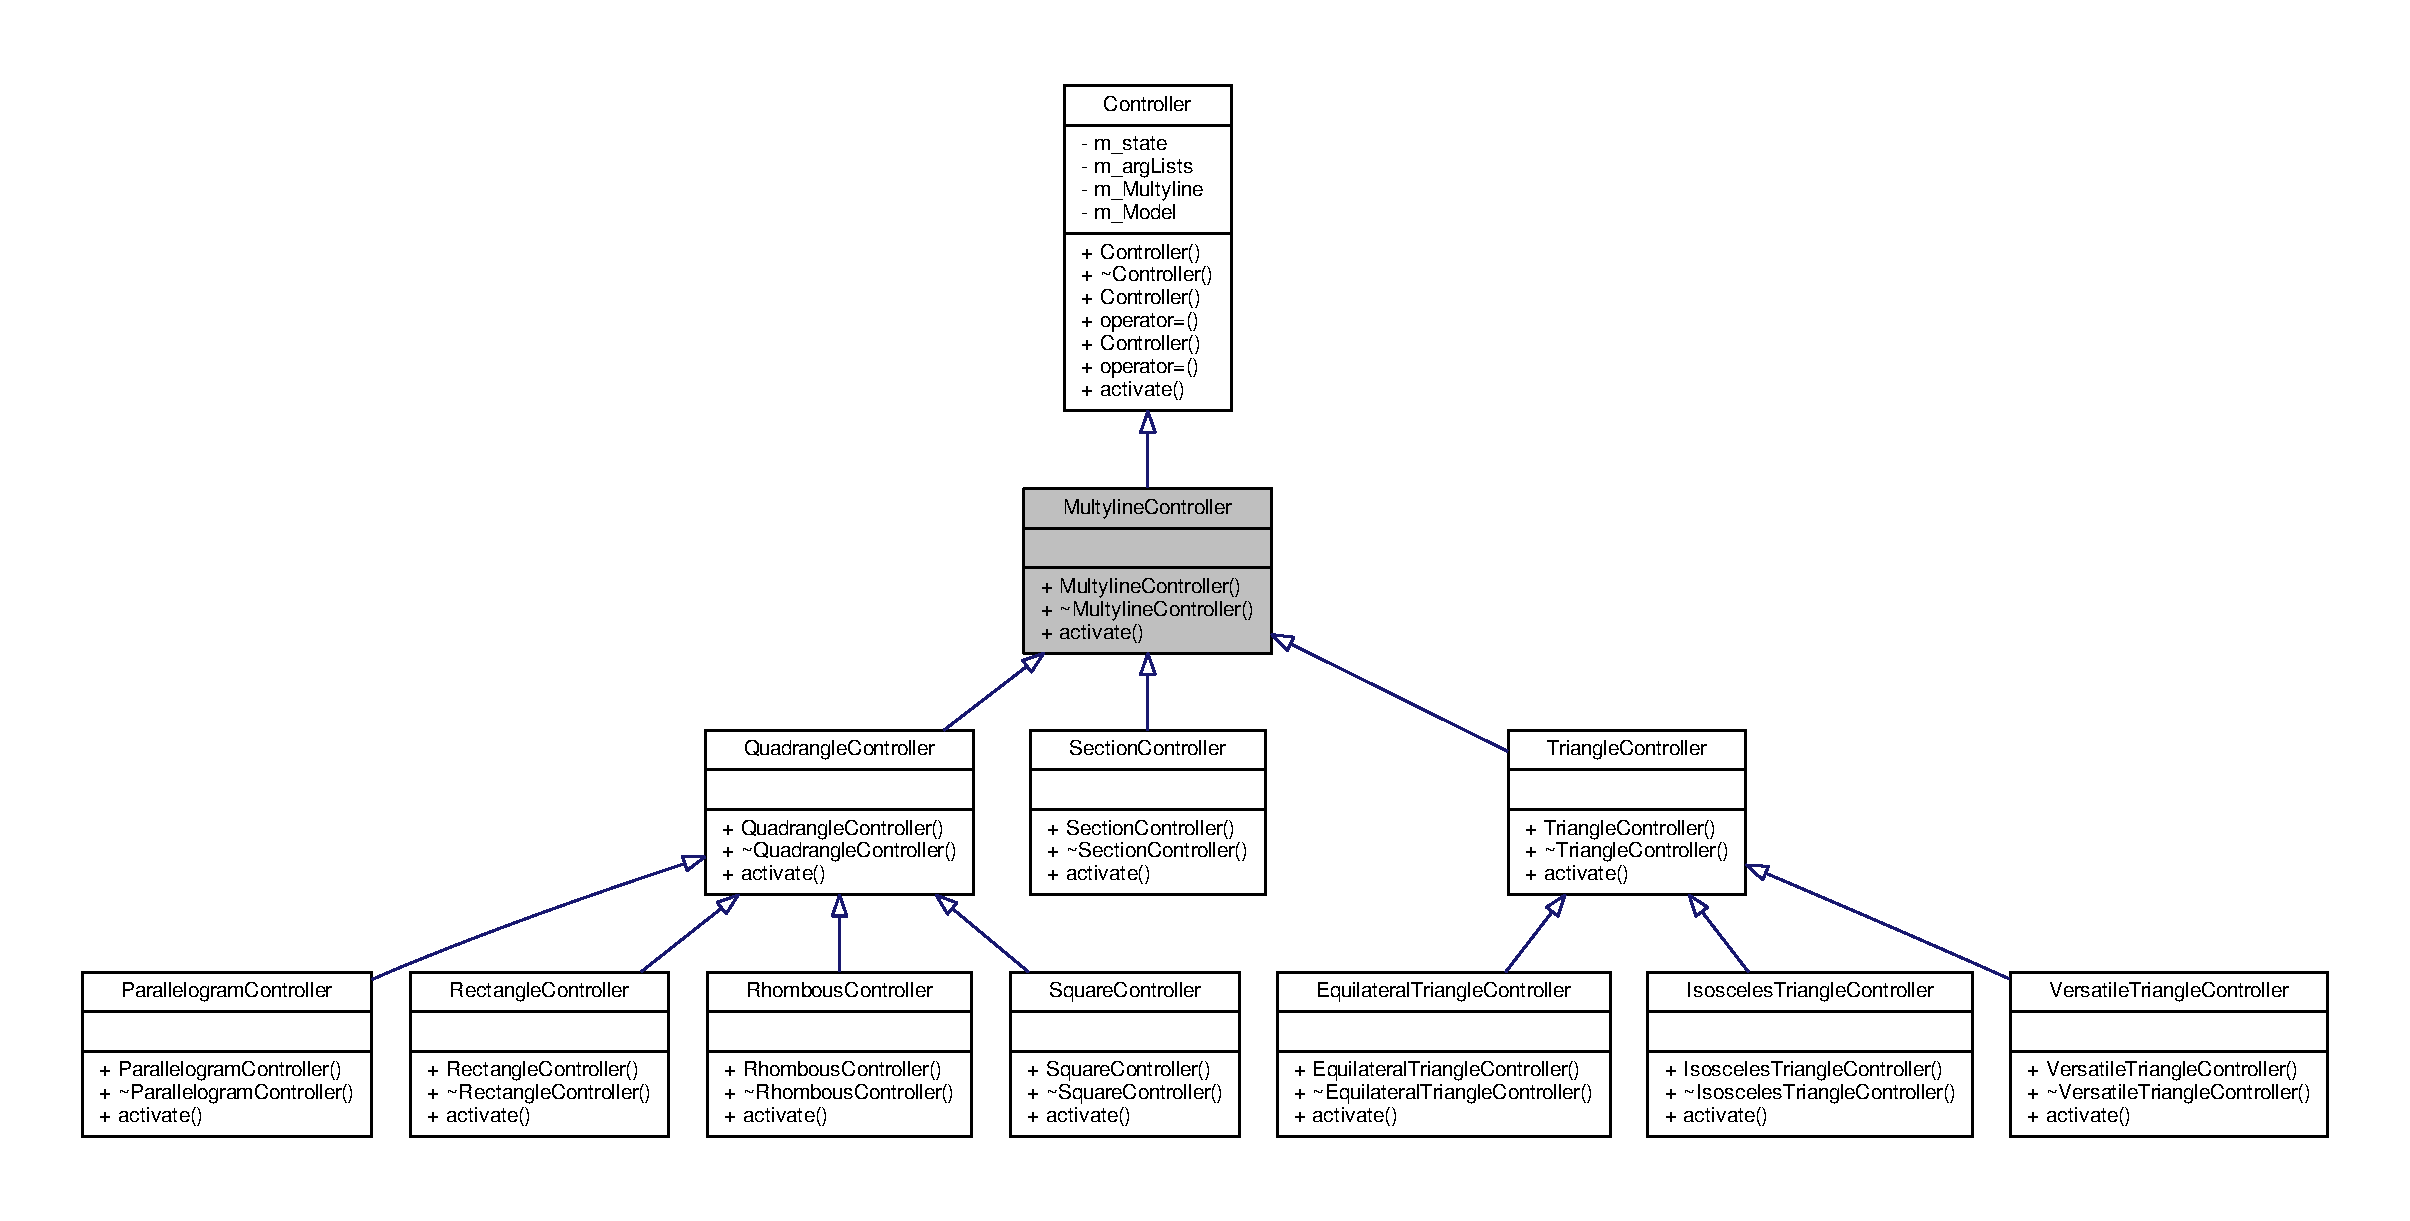
\includegraphics[width=350pt]{class_multyline_controller__inherit__graph}
\end{center}
\end{figure}


Граф связей класса Multyline\-Controller\-:
\nopagebreak
\begin{figure}[H]
\begin{center}
\leavevmode
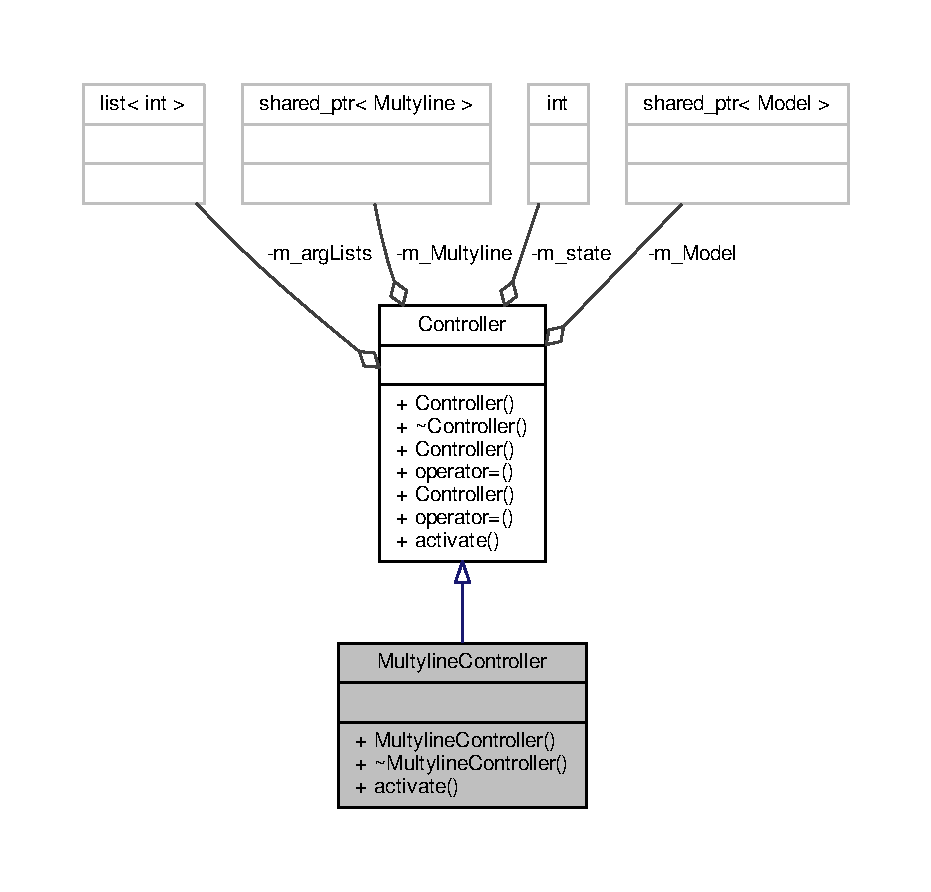
\includegraphics[width=350pt]{class_multyline_controller__coll__graph}
\end{center}
\end{figure}
\subsection*{Открытые члены}
\begin{DoxyCompactItemize}
\item 
\hyperlink{class_multyline_controller_a4a0f4820b82b0c26446a14136ce107b8}{Multyline\-Controller} (std\-::shared\-\_\-ptr$<$ \hyperlink{class_model}{Model} $>$ \&model)
\item 
\hyperlink{class_multyline_controller_a3d5109741986ea4acf16d94e50a47a0f}{$\sim$\-Multyline\-Controller} ()=default
\item 
void \hyperlink{class_multyline_controller_a5a574a5ca48d2a7e62201e9415a61afe}{activate} (int cursor\-Pos\-X, int cursor\-Pos\-Y) override
\end{DoxyCompactItemize}


\subsection{Подробное описание}


См. определение в файле base\-Controller.\-h строка 90



\subsection{Конструктор(ы)}
\hypertarget{class_multyline_controller_a4a0f4820b82b0c26446a14136ce107b8}{\index{Multyline\-Controller@{Multyline\-Controller}!Multyline\-Controller@{Multyline\-Controller}}
\index{Multyline\-Controller@{Multyline\-Controller}!MultylineController@{Multyline\-Controller}}
\subsubsection[{Multyline\-Controller}]{\setlength{\rightskip}{0pt plus 5cm}Multyline\-Controller\-::\-Multyline\-Controller (
\begin{DoxyParamCaption}
\item[{std\-::shared\-\_\-ptr$<$ {\bf Model} $>$ \&}]{model}
\end{DoxyParamCaption}
)\hspace{0.3cm}{\ttfamily [inline]}}}\label{class_multyline_controller_a4a0f4820b82b0c26446a14136ce107b8}


См. определение в файле base\-Controller.\-h строка 93

\hypertarget{class_multyline_controller_a3d5109741986ea4acf16d94e50a47a0f}{\index{Multyline\-Controller@{Multyline\-Controller}!$\sim$\-Multyline\-Controller@{$\sim$\-Multyline\-Controller}}
\index{$\sim$\-Multyline\-Controller@{$\sim$\-Multyline\-Controller}!MultylineController@{Multyline\-Controller}}
\subsubsection[{$\sim$\-Multyline\-Controller}]{\setlength{\rightskip}{0pt plus 5cm}Multyline\-Controller\-::$\sim$\-Multyline\-Controller (
\begin{DoxyParamCaption}
{}
\end{DoxyParamCaption}
)\hspace{0.3cm}{\ttfamily [default]}}}\label{class_multyline_controller_a3d5109741986ea4acf16d94e50a47a0f}


\subsection{Методы}
\hypertarget{class_multyline_controller_a5a574a5ca48d2a7e62201e9415a61afe}{\index{Multyline\-Controller@{Multyline\-Controller}!activate@{activate}}
\index{activate@{activate}!MultylineController@{Multyline\-Controller}}
\subsubsection[{activate}]{\setlength{\rightskip}{0pt plus 5cm}void Multyline\-Controller\-::activate (
\begin{DoxyParamCaption}
\item[{int}]{cursor\-Pos\-X, }
\item[{int}]{cursor\-Pos\-Y}
\end{DoxyParamCaption}
)\hspace{0.3cm}{\ttfamily [inline]}, {\ttfamily [override]}, {\ttfamily [virtual]}}}\label{class_multyline_controller_a5a574a5ca48d2a7e62201e9415a61afe}


Замещает \hyperlink{class_controller_a4cc69a630011f49efb0c221d617af633}{Controller}.



Переопределяется в \hyperlink{class_parallelogram_controller_a42022d7939a32ef5fcdced235edad018}{Parallelogram\-Controller}, \hyperlink{class_rhombous_controller_a9e839123b8a65d202fb898b6233694b2}{Rhombous\-Controller}, \hyperlink{class_rectangle_controller_ac0d209fecccce59cf9270f7f6facbc06}{Rectangle\-Controller}, \hyperlink{class_square_controller_a169d59d75dd023ed352e7722a3bd2dcc}{Square\-Controller}, \hyperlink{class_quadrangle_controller_a2a38c3afba85014f27041e002cfc7950}{Quadrangle\-Controller}, \hyperlink{class_equilateral_triangle_controller_ac8822ad6419def097652fc8a88426898}{Equilateral\-Triangle\-Controller}, \hyperlink{class_isosceles_triangle_controller_ac060b7bdfdc3c5fc078147e14e31415b}{Isosceles\-Triangle\-Controller}, \hyperlink{class_versatile_triangle_controller_a0d553f2393114a789f3e3964b97dad66}{Versatile\-Triangle\-Controller}, \hyperlink{class_triangle_controller_ab86471e4de39ae99bc6198583d173c7b}{Triangle\-Controller} и \hyperlink{class_section_controller_ac42bb71f574f336a79a2e0a739fbad24}{Section\-Controller}.



См. определение в файле base\-Controller.\-h строка 95



Объявления и описания членов класса находятся в файле\-:\begin{DoxyCompactItemize}
\item 
libs/controllers/\hyperlink{base_controller_8h}{base\-Controller.\-h}\end{DoxyCompactItemize}

\hypertarget{class_parallelogram}{\section{Класс Parallelogram}
\label{class_parallelogram}\index{Parallelogram@{Parallelogram}}
}


{\ttfamily \#include $<$m4\-\_\-basic.\-h$>$}



Граф наследования\-:Parallelogram\-:
\nopagebreak
\begin{figure}[H]
\begin{center}
\leavevmode
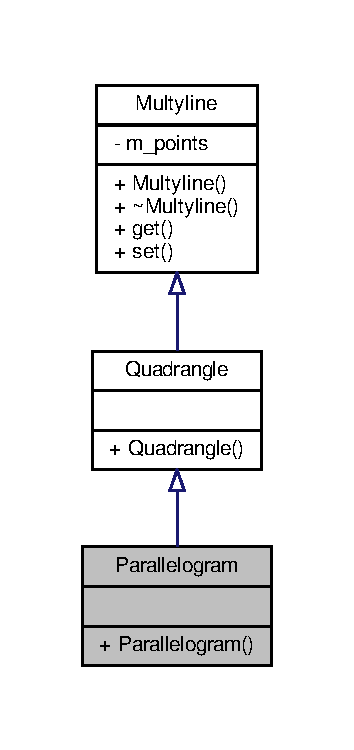
\includegraphics[width=170pt]{class_parallelogram__inherit__graph}
\end{center}
\end{figure}


Граф связей класса Parallelogram\-:
\nopagebreak
\begin{figure}[H]
\begin{center}
\leavevmode
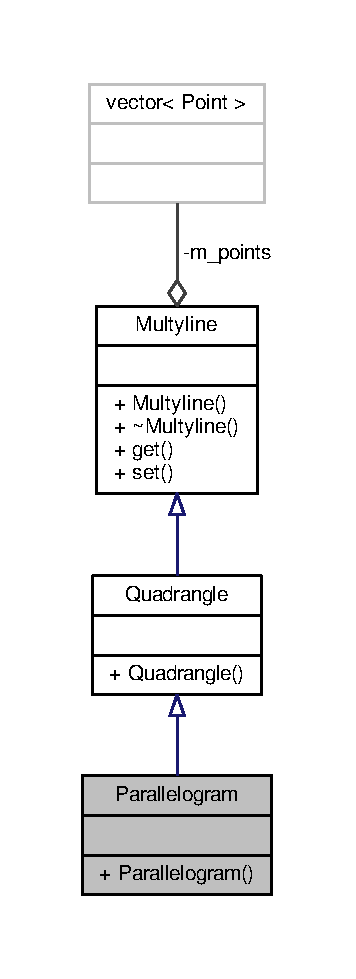
\includegraphics[width=171pt]{class_parallelogram__coll__graph}
\end{center}
\end{figure}
\subsection*{Открытые типы}
\begin{DoxyCompactItemize}
\item 
enum \hyperlink{class_parallelogram_aeae756ed193db05daf0aeb3d0a0966b0}{draw\-Method} \{ \hyperlink{class_parallelogram_aeae756ed193db05daf0aeb3d0a0966b0a8da001730608d2059c34abe87159e366}{point3}, 
\hyperlink{class_parallelogram_aeae756ed193db05daf0aeb3d0a0966b0a1120a1b801f1081028e8345091b6c0b6}{point2}, 
\hyperlink{class_parallelogram_aeae756ed193db05daf0aeb3d0a0966b0a1038e30d507cb7f800b0b3698312be0e}{point1}
 \}
\end{DoxyCompactItemize}
\subsection*{Открытые члены}
\begin{DoxyCompactItemize}
\item 
\hyperlink{class_parallelogram_a430c0f9f5ed2cf85e4c3c2e961be7c2d}{Parallelogram} (\hyperlink{class_multyline_ad75d7bb224267d0d7b4c40fd72a1d920}{draw\-Method}, std\-::initializer\-\_\-list$<$ double $>$ \&)
\end{DoxyCompactItemize}


\subsection{Подробное описание}


См. определение в файле m4\-\_\-basic.\-h строка 72



\subsection{Перечисления}
\hypertarget{class_parallelogram_aeae756ed193db05daf0aeb3d0a0966b0}{\index{Parallelogram@{Parallelogram}!draw\-Method@{draw\-Method}}
\index{draw\-Method@{draw\-Method}!Parallelogram@{Parallelogram}}
\subsubsection[{draw\-Method}]{\setlength{\rightskip}{0pt plus 5cm}enum {\bf Parallelogram\-::draw\-Method}}}\label{class_parallelogram_aeae756ed193db05daf0aeb3d0a0966b0}
\begin{Desc}
\item[Элементы перечислений]\par
\begin{description}
\index{point3@{point3}!Parallelogram@{Parallelogram}}\index{Parallelogram@{Parallelogram}!point3@{point3}}\item[{\em 
\hypertarget{class_parallelogram_aeae756ed193db05daf0aeb3d0a0966b0a8da001730608d2059c34abe87159e366}{point3}\label{class_parallelogram_aeae756ed193db05daf0aeb3d0a0966b0a8da001730608d2059c34abe87159e366}
}]\index{point2@{point2}!Parallelogram@{Parallelogram}}\index{Parallelogram@{Parallelogram}!point2@{point2}}\item[{\em 
\hypertarget{class_parallelogram_aeae756ed193db05daf0aeb3d0a0966b0a1120a1b801f1081028e8345091b6c0b6}{point2}\label{class_parallelogram_aeae756ed193db05daf0aeb3d0a0966b0a1120a1b801f1081028e8345091b6c0b6}
}]\index{point1@{point1}!Parallelogram@{Parallelogram}}\index{Parallelogram@{Parallelogram}!point1@{point1}}\item[{\em 
\hypertarget{class_parallelogram_aeae756ed193db05daf0aeb3d0a0966b0a1038e30d507cb7f800b0b3698312be0e}{point1}\label{class_parallelogram_aeae756ed193db05daf0aeb3d0a0966b0a1038e30d507cb7f800b0b3698312be0e}
}]\end{description}
\end{Desc}


См. определение в файле m4\-\_\-basic.\-h строка 75



\subsection{Конструктор(ы)}
\hypertarget{class_parallelogram_a430c0f9f5ed2cf85e4c3c2e961be7c2d}{\index{Parallelogram@{Parallelogram}!Parallelogram@{Parallelogram}}
\index{Parallelogram@{Parallelogram}!Parallelogram@{Parallelogram}}
\subsubsection[{Parallelogram}]{\setlength{\rightskip}{0pt plus 5cm}Parallelogram\-::\-Parallelogram (
\begin{DoxyParamCaption}
\item[{{\bf draw\-Method}}]{, }
\item[{std\-::initializer\-\_\-list$<$ double $>$ \&}]{}
\end{DoxyParamCaption}
)}}\label{class_parallelogram_a430c0f9f5ed2cf85e4c3c2e961be7c2d}


Объявления и описания членов класса находятся в файле\-:\begin{DoxyCompactItemize}
\item 
libs/models/m\-\_\-shapes/\hyperlink{m4__basic_8h}{m4\-\_\-basic.\-h}\end{DoxyCompactItemize}

\hypertarget{class_parallelogram_controller}{\section{Класс Parallelogram\-Controller}
\label{class_parallelogram_controller}\index{Parallelogram\-Controller@{Parallelogram\-Controller}}
}


{\ttfamily \#include $<$base\-Controller.\-h$>$}



Граф наследования\-:Parallelogram\-Controller\-:
\nopagebreak
\begin{figure}[H]
\begin{center}
\leavevmode
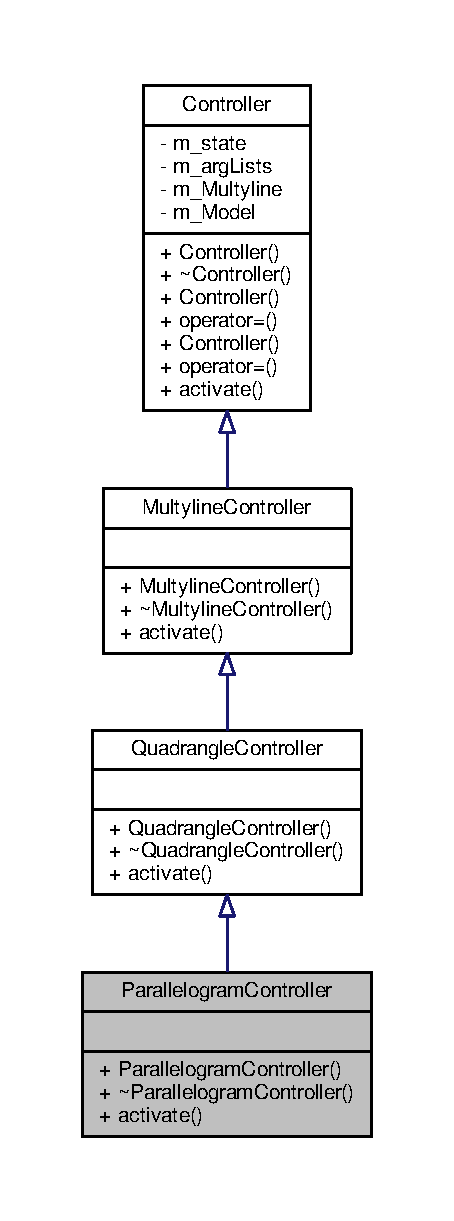
\includegraphics[height=550pt]{class_parallelogram_controller__inherit__graph}
\end{center}
\end{figure}


Граф связей класса Parallelogram\-Controller\-:
\nopagebreak
\begin{figure}[H]
\begin{center}
\leavevmode
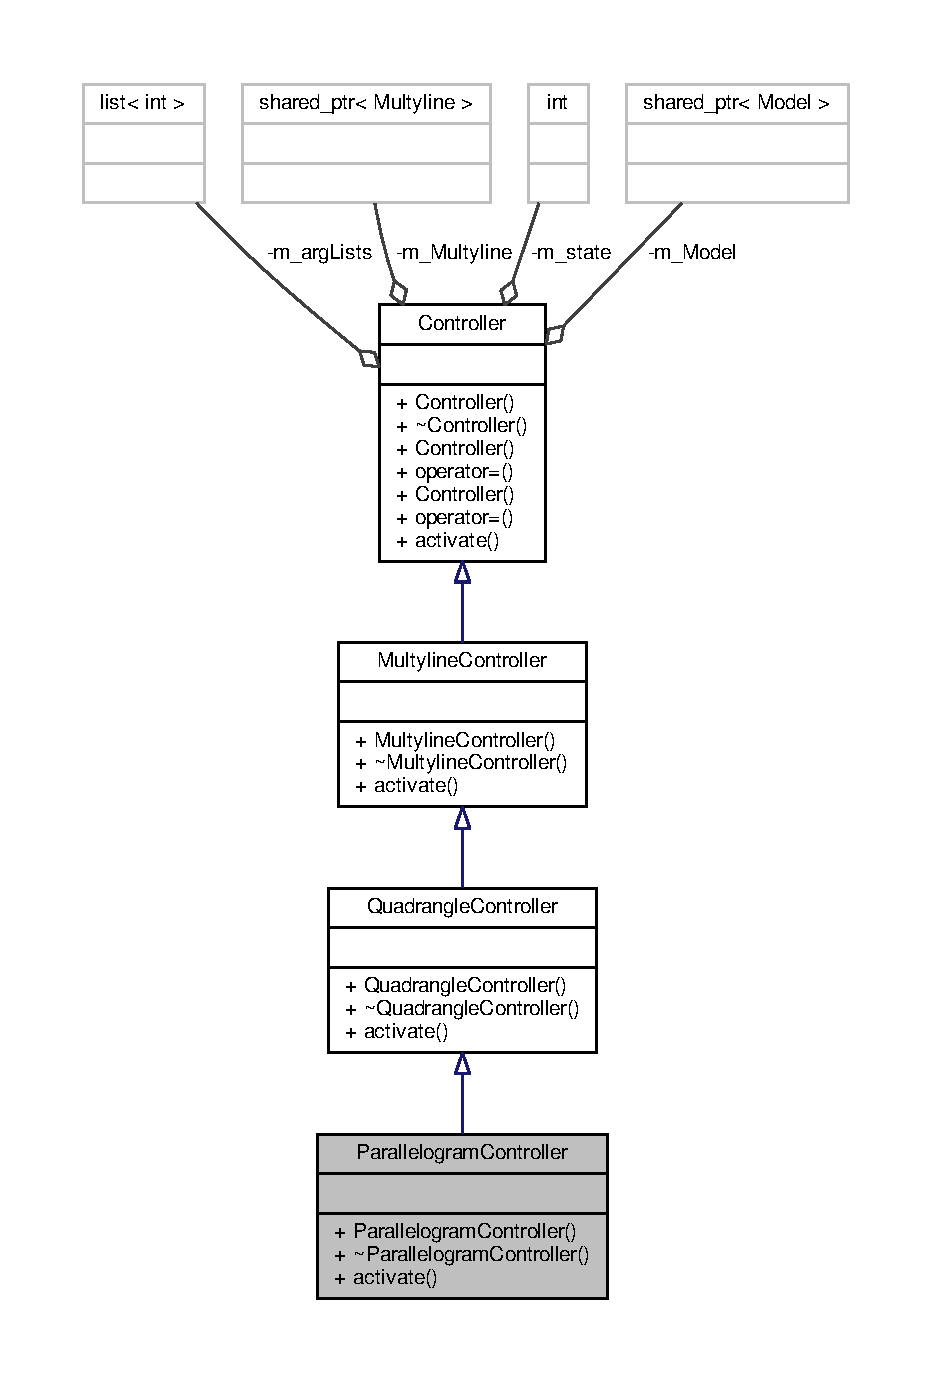
\includegraphics[width=350pt]{class_parallelogram_controller__coll__graph}
\end{center}
\end{figure}
\subsection*{Открытые члены}
\begin{DoxyCompactItemize}
\item 
\hyperlink{class_parallelogram_controller_a50710c8414ccc4dc61ea8feca061b72b}{Parallelogram\-Controller} (std\-::shared\-\_\-ptr$<$ \hyperlink{class_model}{Model} $>$ \&model)
\item 
\hyperlink{class_parallelogram_controller_a5db7cdfa39aed1a197640390917eb4a5}{$\sim$\-Parallelogram\-Controller} ()=default
\item 
void \hyperlink{class_parallelogram_controller_a42022d7939a32ef5fcdced235edad018}{activate} (int cursor\-Pos\-X, int cursor\-Pos\-Y) final
\end{DoxyCompactItemize}


\subsection{Подробное описание}


См. определение в файле base\-Controller.\-h строка 224



\subsection{Конструктор(ы)}
\hypertarget{class_parallelogram_controller_a50710c8414ccc4dc61ea8feca061b72b}{\index{Parallelogram\-Controller@{Parallelogram\-Controller}!Parallelogram\-Controller@{Parallelogram\-Controller}}
\index{Parallelogram\-Controller@{Parallelogram\-Controller}!ParallelogramController@{Parallelogram\-Controller}}
\subsubsection[{Parallelogram\-Controller}]{\setlength{\rightskip}{0pt plus 5cm}Parallelogram\-Controller\-::\-Parallelogram\-Controller (
\begin{DoxyParamCaption}
\item[{std\-::shared\-\_\-ptr$<$ {\bf Model} $>$ \&}]{model}
\end{DoxyParamCaption}
)\hspace{0.3cm}{\ttfamily [inline]}}}\label{class_parallelogram_controller_a50710c8414ccc4dc61ea8feca061b72b}


См. определение в файле base\-Controller.\-h строка 227

\hypertarget{class_parallelogram_controller_a5db7cdfa39aed1a197640390917eb4a5}{\index{Parallelogram\-Controller@{Parallelogram\-Controller}!$\sim$\-Parallelogram\-Controller@{$\sim$\-Parallelogram\-Controller}}
\index{$\sim$\-Parallelogram\-Controller@{$\sim$\-Parallelogram\-Controller}!ParallelogramController@{Parallelogram\-Controller}}
\subsubsection[{$\sim$\-Parallelogram\-Controller}]{\setlength{\rightskip}{0pt plus 5cm}Parallelogram\-Controller\-::$\sim$\-Parallelogram\-Controller (
\begin{DoxyParamCaption}
{}
\end{DoxyParamCaption}
)\hspace{0.3cm}{\ttfamily [default]}}}\label{class_parallelogram_controller_a5db7cdfa39aed1a197640390917eb4a5}


\subsection{Методы}
\hypertarget{class_parallelogram_controller_a42022d7939a32ef5fcdced235edad018}{\index{Parallelogram\-Controller@{Parallelogram\-Controller}!activate@{activate}}
\index{activate@{activate}!ParallelogramController@{Parallelogram\-Controller}}
\subsubsection[{activate}]{\setlength{\rightskip}{0pt plus 5cm}void Parallelogram\-Controller\-::activate (
\begin{DoxyParamCaption}
\item[{int}]{cursor\-Pos\-X, }
\item[{int}]{cursor\-Pos\-Y}
\end{DoxyParamCaption}
)\hspace{0.3cm}{\ttfamily [inline]}, {\ttfamily [final]}, {\ttfamily [virtual]}}}\label{class_parallelogram_controller_a42022d7939a32ef5fcdced235edad018}


Переопределяет метод предка \hyperlink{class_quadrangle_controller_a2a38c3afba85014f27041e002cfc7950}{Quadrangle\-Controller}.



См. определение в файле base\-Controller.\-h строка 229



Объявления и описания членов класса находятся в файле\-:\begin{DoxyCompactItemize}
\item 
libs/controllers/\hyperlink{base_controller_8h}{base\-Controller.\-h}\end{DoxyCompactItemize}

\hypertarget{class_point}{\section{Класс Point}
\label{class_point}\index{Point@{Point}}
}


{\ttfamily \#include $<$m\-\_\-point.\-h$>$}



Граф связей класса Point\-:
\nopagebreak
\begin{figure}[H]
\begin{center}
\leavevmode
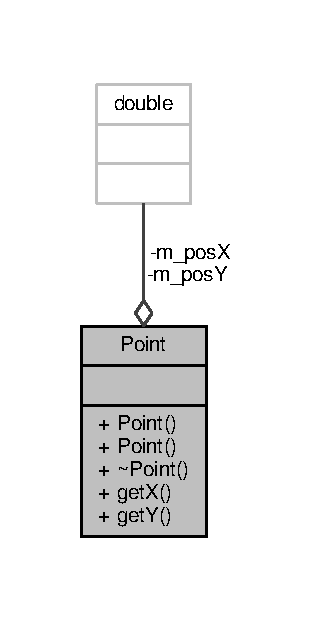
\includegraphics[width=152pt]{class_point__coll__graph}
\end{center}
\end{figure}
\subsection*{Открытые члены}
\begin{DoxyCompactItemize}
\item 
\hyperlink{class_point_ad92f2337b839a94ce97dcdb439b4325a}{Point} ()
\item 
\hyperlink{class_point_a483cf6bf601889eb922e89f5820045c1}{Point} (double \-\_\-x, double \-\_\-y)
\item 
\hyperlink{class_point_aa1fcbfbf1e997b4f6bd064afeda495f7}{$\sim$\-Point} ()=default
\item 
const double \& \hyperlink{class_point_aca563d76886a7b127077a84586fb055c}{get\-X} ()
\item 
const double \& \hyperlink{class_point_a8a1fb1c5a1201858679a55dd9515f5ae}{get\-Y} ()
\end{DoxyCompactItemize}
\subsection*{Закрытые данные}
\begin{DoxyCompactItemize}
\item 
double \hyperlink{class_point_a6bc233f75b7f95673756301323bc7e82}{m\-\_\-pos\-X}
\item 
double \hyperlink{class_point_a9cf23d4ad95854a89a4b0228f4cd7290}{m\-\_\-pos\-Y}
\end{DoxyCompactItemize}


\subsection{Подробное описание}


См. определение в файле m\-\_\-point.\-h строка 6



\subsection{Конструктор(ы)}
\hypertarget{class_point_ad92f2337b839a94ce97dcdb439b4325a}{\index{Point@{Point}!Point@{Point}}
\index{Point@{Point}!Point@{Point}}
\subsubsection[{Point}]{\setlength{\rightskip}{0pt plus 5cm}Point\-::\-Point (
\begin{DoxyParamCaption}
{}
\end{DoxyParamCaption}
)\hspace{0.3cm}{\ttfamily [inline]}}}\label{class_point_ad92f2337b839a94ce97dcdb439b4325a}


См. определение в файле m\-\_\-point.\-h строка 9

\hypertarget{class_point_a483cf6bf601889eb922e89f5820045c1}{\index{Point@{Point}!Point@{Point}}
\index{Point@{Point}!Point@{Point}}
\subsubsection[{Point}]{\setlength{\rightskip}{0pt plus 5cm}Point\-::\-Point (
\begin{DoxyParamCaption}
\item[{double}]{\-\_\-x, }
\item[{double}]{\-\_\-y}
\end{DoxyParamCaption}
)\hspace{0.3cm}{\ttfamily [inline]}}}\label{class_point_a483cf6bf601889eb922e89f5820045c1}


См. определение в файле m\-\_\-point.\-h строка 11

\hypertarget{class_point_aa1fcbfbf1e997b4f6bd064afeda495f7}{\index{Point@{Point}!$\sim$\-Point@{$\sim$\-Point}}
\index{$\sim$\-Point@{$\sim$\-Point}!Point@{Point}}
\subsubsection[{$\sim$\-Point}]{\setlength{\rightskip}{0pt plus 5cm}Point\-::$\sim$\-Point (
\begin{DoxyParamCaption}
{}
\end{DoxyParamCaption}
)\hspace{0.3cm}{\ttfamily [default]}}}\label{class_point_aa1fcbfbf1e997b4f6bd064afeda495f7}


\subsection{Методы}
\hypertarget{class_point_aca563d76886a7b127077a84586fb055c}{\index{Point@{Point}!get\-X@{get\-X}}
\index{get\-X@{get\-X}!Point@{Point}}
\subsubsection[{get\-X}]{\setlength{\rightskip}{0pt plus 5cm}const double\& Point\-::get\-X (
\begin{DoxyParamCaption}
{}
\end{DoxyParamCaption}
)\hspace{0.3cm}{\ttfamily [inline]}}}\label{class_point_aca563d76886a7b127077a84586fb055c}


См. определение в файле m\-\_\-point.\-h строка 14

\hypertarget{class_point_a8a1fb1c5a1201858679a55dd9515f5ae}{\index{Point@{Point}!get\-Y@{get\-Y}}
\index{get\-Y@{get\-Y}!Point@{Point}}
\subsubsection[{get\-Y}]{\setlength{\rightskip}{0pt plus 5cm}const double\& Point\-::get\-Y (
\begin{DoxyParamCaption}
{}
\end{DoxyParamCaption}
)\hspace{0.3cm}{\ttfamily [inline]}}}\label{class_point_a8a1fb1c5a1201858679a55dd9515f5ae}


См. определение в файле m\-\_\-point.\-h строка 15



\subsection{Данные класса}
\hypertarget{class_point_a6bc233f75b7f95673756301323bc7e82}{\index{Point@{Point}!m\-\_\-pos\-X@{m\-\_\-pos\-X}}
\index{m\-\_\-pos\-X@{m\-\_\-pos\-X}!Point@{Point}}
\subsubsection[{m\-\_\-pos\-X}]{\setlength{\rightskip}{0pt plus 5cm}double Point\-::m\-\_\-pos\-X\hspace{0.3cm}{\ttfamily [private]}}}\label{class_point_a6bc233f75b7f95673756301323bc7e82}


См. определение в файле m\-\_\-point.\-h строка 15

\hypertarget{class_point_a9cf23d4ad95854a89a4b0228f4cd7290}{\index{Point@{Point}!m\-\_\-pos\-Y@{m\-\_\-pos\-Y}}
\index{m\-\_\-pos\-Y@{m\-\_\-pos\-Y}!Point@{Point}}
\subsubsection[{m\-\_\-pos\-Y}]{\setlength{\rightskip}{0pt plus 5cm}double Point\-::m\-\_\-pos\-Y\hspace{0.3cm}{\ttfamily [private]}}}\label{class_point_a9cf23d4ad95854a89a4b0228f4cd7290}


См. определение в файле m\-\_\-point.\-h строка 19



Объявления и описания членов класса находятся в файле\-:\begin{DoxyCompactItemize}
\item 
libs/models/\hyperlink{m__point_8h}{m\-\_\-point.\-h}\end{DoxyCompactItemize}

\hypertarget{class_quadrangle}{\section{Класс Quadrangle}
\label{class_quadrangle}\index{Quadrangle@{Quadrangle}}
}


{\ttfamily \#include $<$m4\-\_\-basic.\-h$>$}



Граф наследования\-:Quadrangle\-:
\nopagebreak
\begin{figure}[H]
\begin{center}
\leavevmode
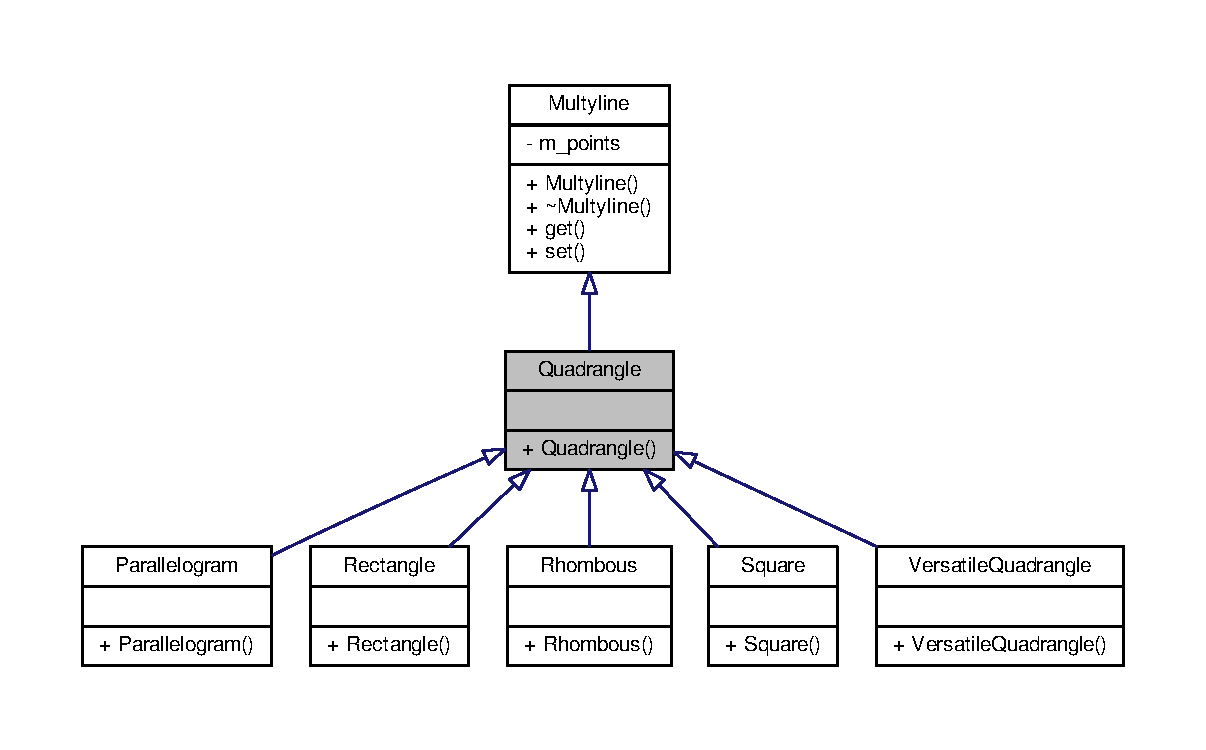
\includegraphics[width=350pt]{class_quadrangle__inherit__graph}
\end{center}
\end{figure}


Граф связей класса Quadrangle\-:
\nopagebreak
\begin{figure}[H]
\begin{center}
\leavevmode
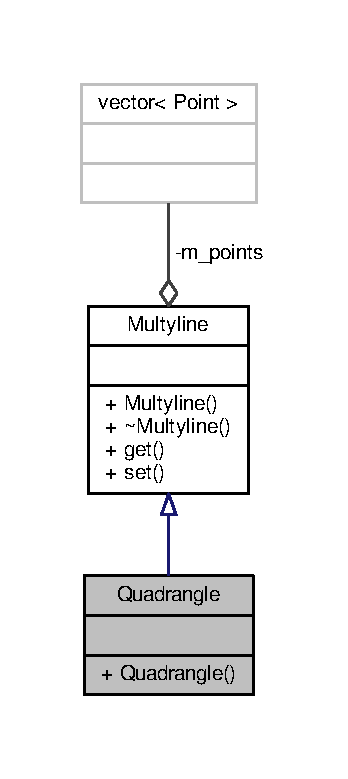
\includegraphics[width=167pt]{class_quadrangle__coll__graph}
\end{center}
\end{figure}
\subsection*{Открытые члены}
\begin{DoxyCompactItemize}
\item 
\hyperlink{class_quadrangle_a8b4e36be41d7934614c333776c052736}{Quadrangle} (std\-::initializer\-\_\-list$<$ double $>$ \&points)
\end{DoxyCompactItemize}
\subsection*{Дополнительные унаследованные члены}


\subsection{Подробное описание}


См. определение в файле m4\-\_\-basic.\-h строка 6



\subsection{Конструктор(ы)}
\hypertarget{class_quadrangle_a8b4e36be41d7934614c333776c052736}{\index{Quadrangle@{Quadrangle}!Quadrangle@{Quadrangle}}
\index{Quadrangle@{Quadrangle}!Quadrangle@{Quadrangle}}
\subsubsection[{Quadrangle}]{\setlength{\rightskip}{0pt plus 5cm}Quadrangle\-::\-Quadrangle (
\begin{DoxyParamCaption}
\item[{std\-::initializer\-\_\-list$<$ double $>$ \&}]{points}
\end{DoxyParamCaption}
)\hspace{0.3cm}{\ttfamily [inline]}}}\label{class_quadrangle_a8b4e36be41d7934614c333776c052736}


См. определение в файле m4\-\_\-basic.\-h строка 9



Объявления и описания членов класса находятся в файле\-:\begin{DoxyCompactItemize}
\item 
libs/models/m\-\_\-shapes/\hyperlink{m4__basic_8h}{m4\-\_\-basic.\-h}\end{DoxyCompactItemize}

\hypertarget{class_quadrangle_controller}{\section{Класс Quadrangle\-Controller}
\label{class_quadrangle_controller}\index{Quadrangle\-Controller@{Quadrangle\-Controller}}
}


{\ttfamily \#include $<$base\-Controller.\-h$>$}



Граф наследования\-:Quadrangle\-Controller\-:
\nopagebreak
\begin{figure}[H]
\begin{center}
\leavevmode
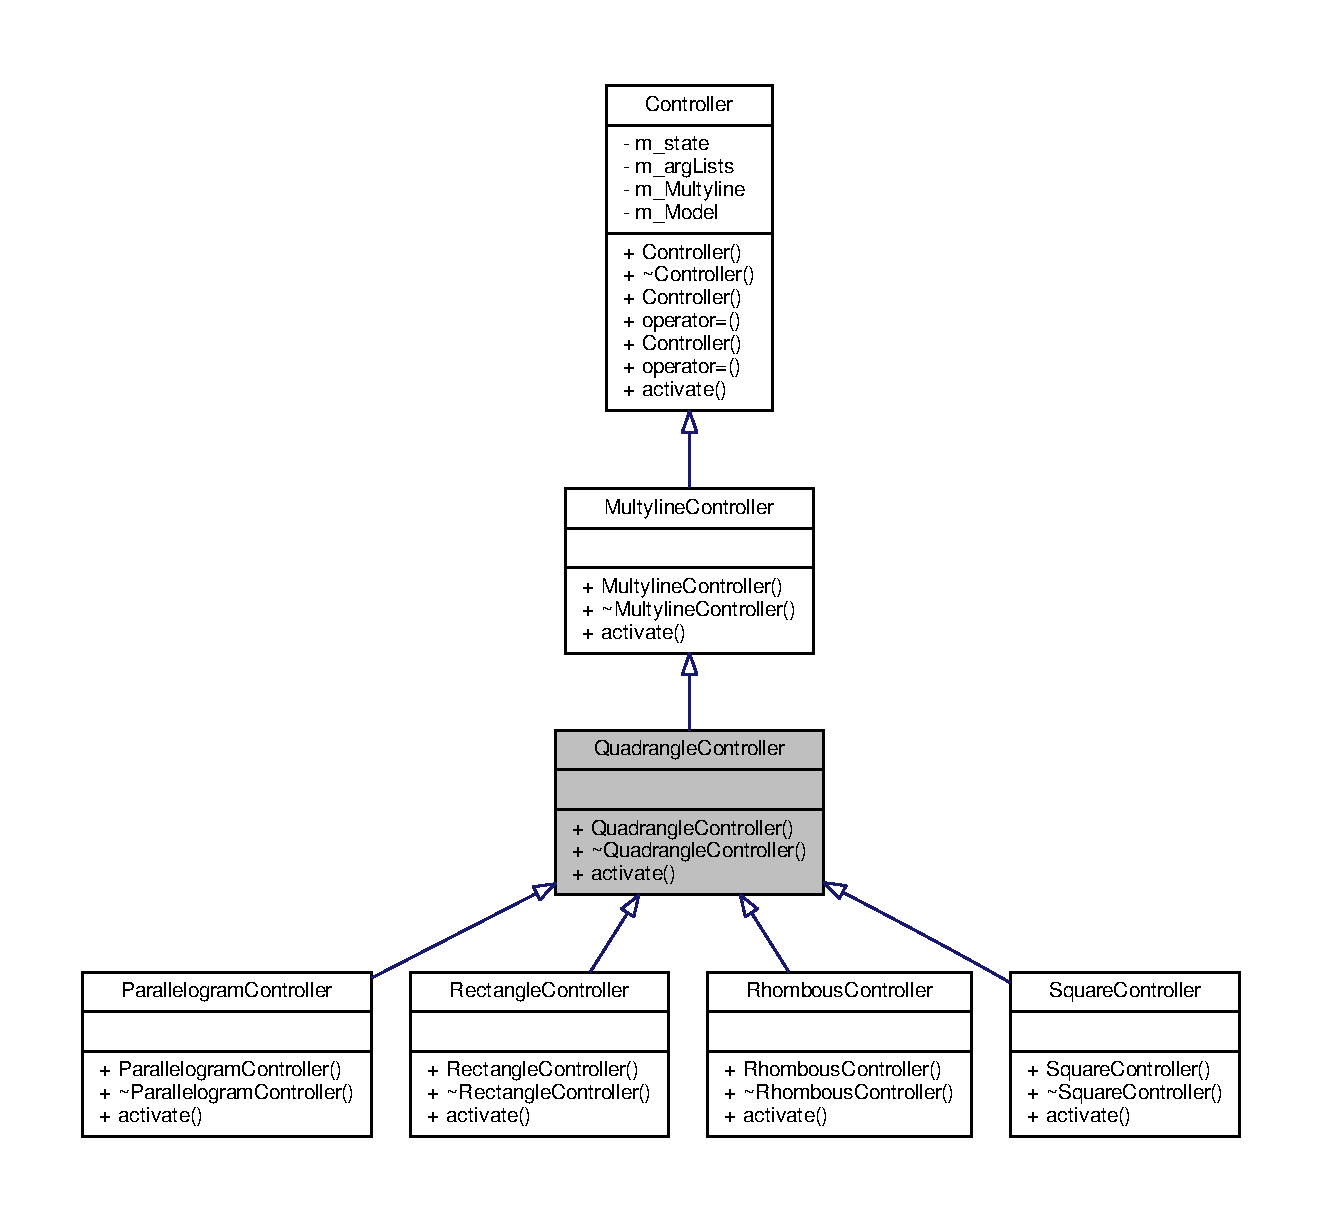
\includegraphics[width=350pt]{class_quadrangle_controller__inherit__graph}
\end{center}
\end{figure}


Граф связей класса Quadrangle\-Controller\-:
\nopagebreak
\begin{figure}[H]
\begin{center}
\leavevmode
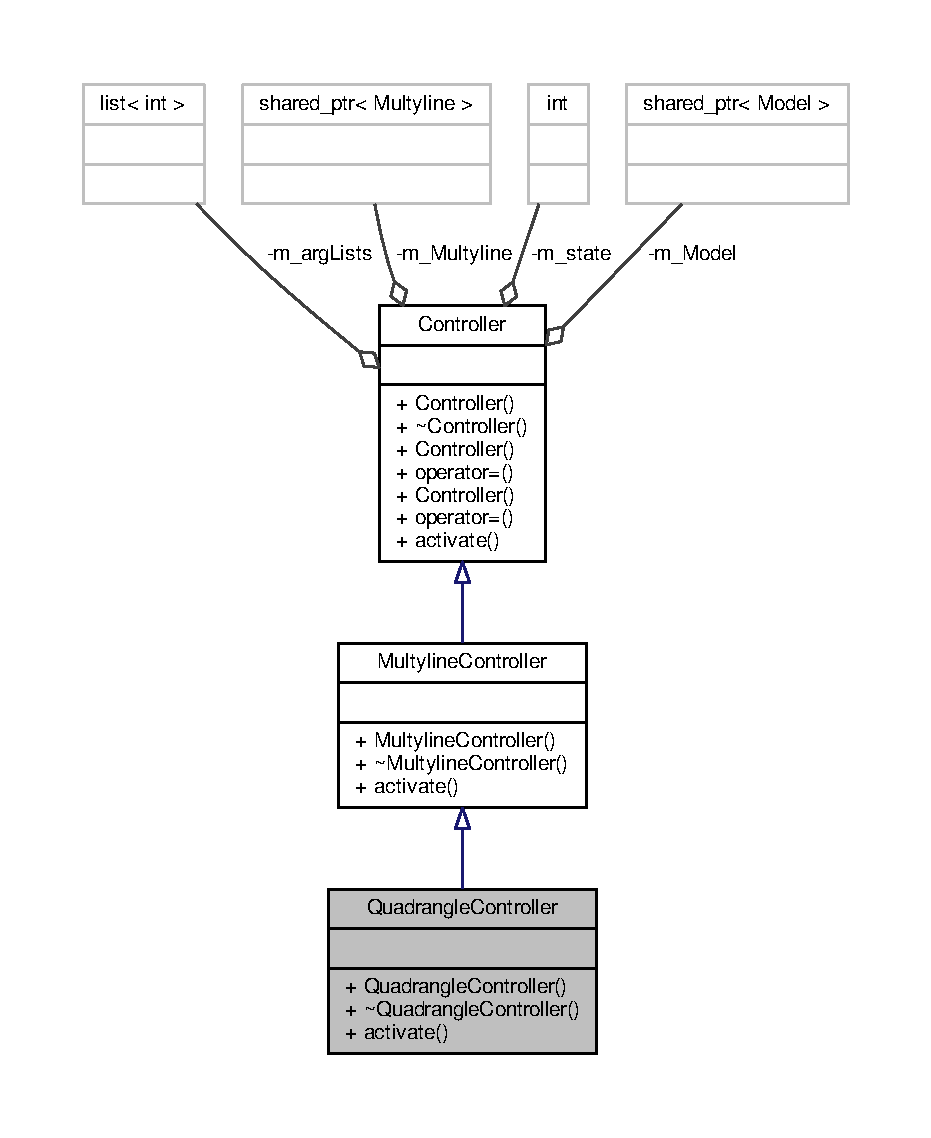
\includegraphics[width=350pt]{class_quadrangle_controller__coll__graph}
\end{center}
\end{figure}
\subsection*{Открытые члены}
\begin{DoxyCompactItemize}
\item 
\hyperlink{class_quadrangle_controller_a36a3a0fdae528a6ad785a22563eff2a0}{Quadrangle\-Controller} (std\-::shared\-\_\-ptr$<$ \hyperlink{class_model}{Model} $>$ \&model)
\item 
virtual \hyperlink{class_quadrangle_controller_a2c8f69d0c8f1e740e06fd9d754f30a99}{$\sim$\-Quadrangle\-Controller} ()=default
\item 
void \hyperlink{class_quadrangle_controller_a2a38c3afba85014f27041e002cfc7950}{activate} (int cursor\-Pos\-X, int cursor\-Pos\-Y) override
\end{DoxyCompactItemize}


\subsection{Подробное описание}


См. определение в файле base\-Controller.\-h строка 172



\subsection{Конструктор(ы)}
\hypertarget{class_quadrangle_controller_a36a3a0fdae528a6ad785a22563eff2a0}{\index{Quadrangle\-Controller@{Quadrangle\-Controller}!Quadrangle\-Controller@{Quadrangle\-Controller}}
\index{Quadrangle\-Controller@{Quadrangle\-Controller}!QuadrangleController@{Quadrangle\-Controller}}
\subsubsection[{Quadrangle\-Controller}]{\setlength{\rightskip}{0pt plus 5cm}Quadrangle\-Controller\-::\-Quadrangle\-Controller (
\begin{DoxyParamCaption}
\item[{std\-::shared\-\_\-ptr$<$ {\bf Model} $>$ \&}]{model}
\end{DoxyParamCaption}
)\hspace{0.3cm}{\ttfamily [inline]}}}\label{class_quadrangle_controller_a36a3a0fdae528a6ad785a22563eff2a0}


См. определение в файле base\-Controller.\-h строка 175

\hypertarget{class_quadrangle_controller_a2c8f69d0c8f1e740e06fd9d754f30a99}{\index{Quadrangle\-Controller@{Quadrangle\-Controller}!$\sim$\-Quadrangle\-Controller@{$\sim$\-Quadrangle\-Controller}}
\index{$\sim$\-Quadrangle\-Controller@{$\sim$\-Quadrangle\-Controller}!QuadrangleController@{Quadrangle\-Controller}}
\subsubsection[{$\sim$\-Quadrangle\-Controller}]{\setlength{\rightskip}{0pt plus 5cm}virtual Quadrangle\-Controller\-::$\sim$\-Quadrangle\-Controller (
\begin{DoxyParamCaption}
{}
\end{DoxyParamCaption}
)\hspace{0.3cm}{\ttfamily [virtual]}, {\ttfamily [default]}}}\label{class_quadrangle_controller_a2c8f69d0c8f1e740e06fd9d754f30a99}


\subsection{Методы}
\hypertarget{class_quadrangle_controller_a2a38c3afba85014f27041e002cfc7950}{\index{Quadrangle\-Controller@{Quadrangle\-Controller}!activate@{activate}}
\index{activate@{activate}!QuadrangleController@{Quadrangle\-Controller}}
\subsubsection[{activate}]{\setlength{\rightskip}{0pt plus 5cm}void Quadrangle\-Controller\-::activate (
\begin{DoxyParamCaption}
\item[{int}]{cursor\-Pos\-X, }
\item[{int}]{cursor\-Pos\-Y}
\end{DoxyParamCaption}
)\hspace{0.3cm}{\ttfamily [inline]}, {\ttfamily [override]}, {\ttfamily [virtual]}}}\label{class_quadrangle_controller_a2a38c3afba85014f27041e002cfc7950}


Переопределяет метод предка \hyperlink{class_multyline_controller_a5a574a5ca48d2a7e62201e9415a61afe}{Multyline\-Controller}.



Переопределяется в \hyperlink{class_parallelogram_controller_a42022d7939a32ef5fcdced235edad018}{Parallelogram\-Controller}, \hyperlink{class_rhombous_controller_a9e839123b8a65d202fb898b6233694b2}{Rhombous\-Controller}, \hyperlink{class_rectangle_controller_ac0d209fecccce59cf9270f7f6facbc06}{Rectangle\-Controller} и \hyperlink{class_square_controller_a169d59d75dd023ed352e7722a3bd2dcc}{Square\-Controller}.



См. определение в файле base\-Controller.\-h строка 177



Объявления и описания членов класса находятся в файле\-:\begin{DoxyCompactItemize}
\item 
libs/controllers/\hyperlink{base_controller_8h}{base\-Controller.\-h}\end{DoxyCompactItemize}

\hypertarget{class_rectangle}{\section{Класс Rectangle}
\label{class_rectangle}\index{Rectangle@{Rectangle}}
}


{\ttfamily \#include $<$m4\-\_\-basic.\-h$>$}



Граф наследования\-:Rectangle\-:
\nopagebreak
\begin{figure}[H]
\begin{center}
\leavevmode
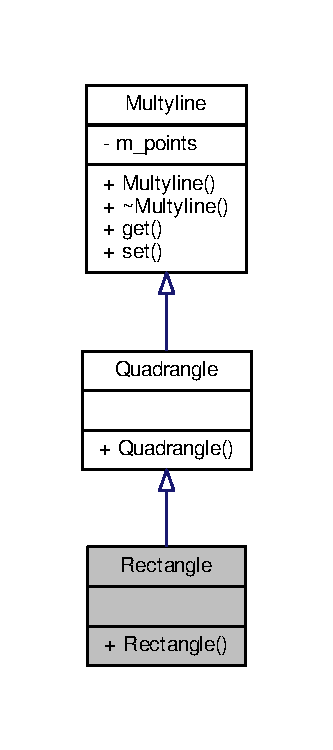
\includegraphics[width=160pt]{class_rectangle__inherit__graph}
\end{center}
\end{figure}


Граф связей класса Rectangle\-:
\nopagebreak
\begin{figure}[H]
\begin{center}
\leavevmode
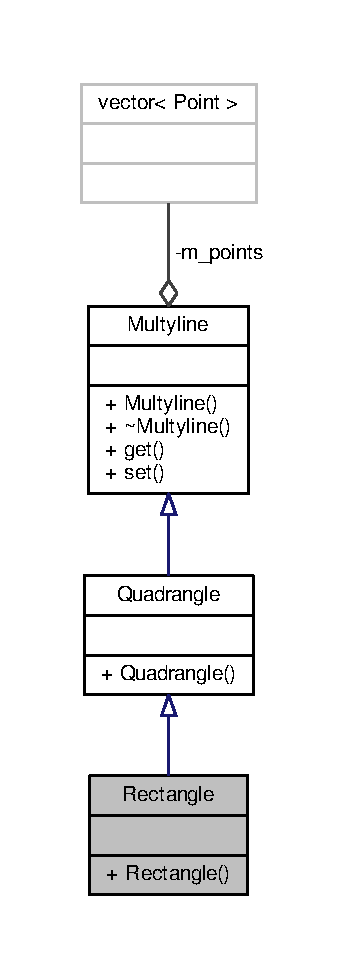
\includegraphics[width=167pt]{class_rectangle__coll__graph}
\end{center}
\end{figure}
\subsection*{Открытые типы}
\begin{DoxyCompactItemize}
\item 
enum \hyperlink{class_rectangle_a89fbf9e00116333aaa820d66f940462f}{draw\-Method} \{ \hyperlink{class_rectangle_a89fbf9e00116333aaa820d66f940462fa0899aa004a2bdd5ca0a442c05a2fdb70}{point3}, 
\hyperlink{class_rectangle_a89fbf9e00116333aaa820d66f940462fa6083fe468bbf9e5a1b0cc8faaf4579f3}{point2}, 
\hyperlink{class_rectangle_a89fbf9e00116333aaa820d66f940462fab936647558e60d8993ec9758f1bee652}{point1}
 \}
\end{DoxyCompactItemize}
\subsection*{Открытые члены}
\begin{DoxyCompactItemize}
\item 
\hyperlink{class_rectangle_a436ec626a20dd8355999fc7d61475c1b}{Rectangle} (\hyperlink{class_multyline_ad75d7bb224267d0d7b4c40fd72a1d920}{draw\-Method}, std\-::initializer\-\_\-list$<$ double $>$ \&)
\end{DoxyCompactItemize}


\subsection{Подробное описание}


См. определение в файле m4\-\_\-basic.\-h строка 36



\subsection{Перечисления}
\hypertarget{class_rectangle_a89fbf9e00116333aaa820d66f940462f}{\index{Rectangle@{Rectangle}!draw\-Method@{draw\-Method}}
\index{draw\-Method@{draw\-Method}!Rectangle@{Rectangle}}
\subsubsection[{draw\-Method}]{\setlength{\rightskip}{0pt plus 5cm}enum {\bf Rectangle\-::draw\-Method}}}\label{class_rectangle_a89fbf9e00116333aaa820d66f940462f}
\begin{Desc}
\item[Элементы перечислений]\par
\begin{description}
\index{point3@{point3}!Rectangle@{Rectangle}}\index{Rectangle@{Rectangle}!point3@{point3}}\item[{\em 
\hypertarget{class_rectangle_a89fbf9e00116333aaa820d66f940462fa0899aa004a2bdd5ca0a442c05a2fdb70}{point3}\label{class_rectangle_a89fbf9e00116333aaa820d66f940462fa0899aa004a2bdd5ca0a442c05a2fdb70}
}]\index{point2@{point2}!Rectangle@{Rectangle}}\index{Rectangle@{Rectangle}!point2@{point2}}\item[{\em 
\hypertarget{class_rectangle_a89fbf9e00116333aaa820d66f940462fa6083fe468bbf9e5a1b0cc8faaf4579f3}{point2}\label{class_rectangle_a89fbf9e00116333aaa820d66f940462fa6083fe468bbf9e5a1b0cc8faaf4579f3}
}]\index{point1@{point1}!Rectangle@{Rectangle}}\index{Rectangle@{Rectangle}!point1@{point1}}\item[{\em 
\hypertarget{class_rectangle_a89fbf9e00116333aaa820d66f940462fab936647558e60d8993ec9758f1bee652}{point1}\label{class_rectangle_a89fbf9e00116333aaa820d66f940462fab936647558e60d8993ec9758f1bee652}
}]\end{description}
\end{Desc}


См. определение в файле m4\-\_\-basic.\-h строка 39



\subsection{Конструктор(ы)}
\hypertarget{class_rectangle_a436ec626a20dd8355999fc7d61475c1b}{\index{Rectangle@{Rectangle}!Rectangle@{Rectangle}}
\index{Rectangle@{Rectangle}!Rectangle@{Rectangle}}
\subsubsection[{Rectangle}]{\setlength{\rightskip}{0pt plus 5cm}Rectangle\-::\-Rectangle (
\begin{DoxyParamCaption}
\item[{{\bf draw\-Method}}]{, }
\item[{std\-::initializer\-\_\-list$<$ double $>$ \&}]{}
\end{DoxyParamCaption}
)}}\label{class_rectangle_a436ec626a20dd8355999fc7d61475c1b}


Объявления и описания членов класса находятся в файле\-:\begin{DoxyCompactItemize}
\item 
libs/models/m\-\_\-shapes/\hyperlink{m4__basic_8h}{m4\-\_\-basic.\-h}\end{DoxyCompactItemize}

\hypertarget{class_rectangle_controller}{\section{Класс Rectangle\-Controller}
\label{class_rectangle_controller}\index{Rectangle\-Controller@{Rectangle\-Controller}}
}


{\ttfamily \#include $<$base\-Controller.\-h$>$}



Граф наследования\-:Rectangle\-Controller\-:
\nopagebreak
\begin{figure}[H]
\begin{center}
\leavevmode
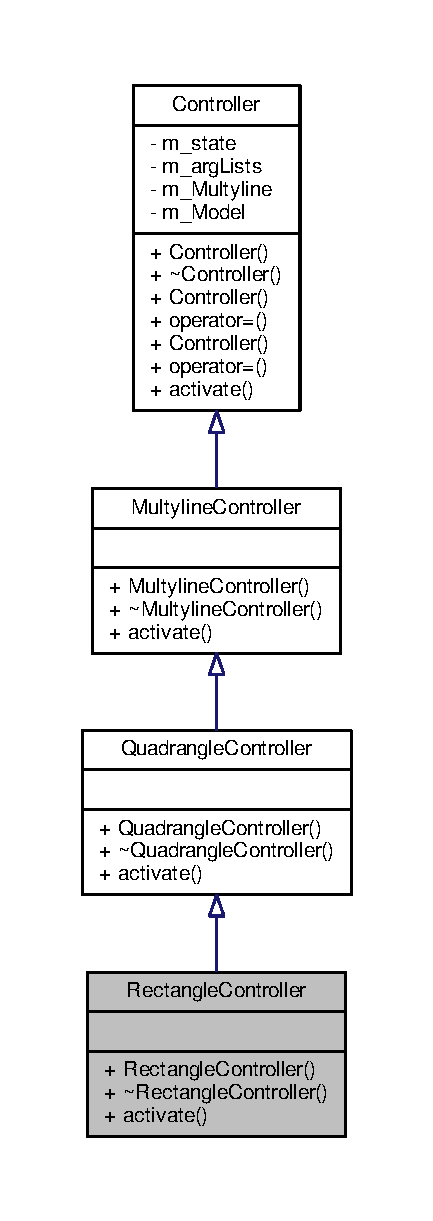
\includegraphics[height=550pt]{class_rectangle_controller__inherit__graph}
\end{center}
\end{figure}


Граф связей класса Rectangle\-Controller\-:
\nopagebreak
\begin{figure}[H]
\begin{center}
\leavevmode
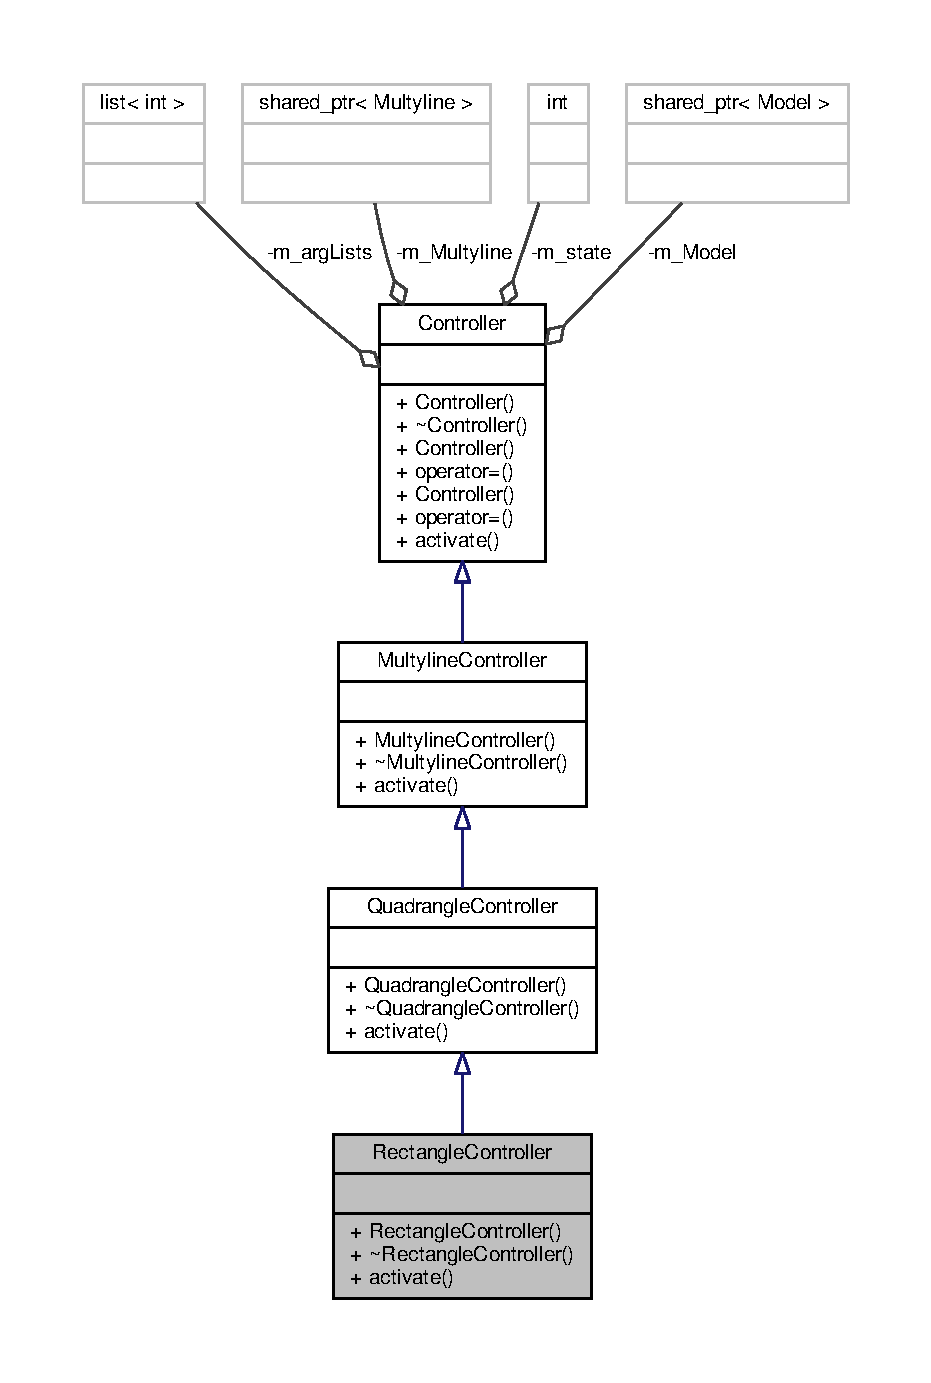
\includegraphics[width=350pt]{class_rectangle_controller__coll__graph}
\end{center}
\end{figure}
\subsection*{Открытые члены}
\begin{DoxyCompactItemize}
\item 
\hyperlink{class_rectangle_controller_a31b4fd49338cbd4cdcadbf4cdc9bb1b7}{Rectangle\-Controller} (std\-::shared\-\_\-ptr$<$ \hyperlink{class_model}{Model} $>$ \&model)
\item 
virtual \hyperlink{class_rectangle_controller_a5bfdcba403d2189aeb7672ec66c9d3e2}{$\sim$\-Rectangle\-Controller} ()=default
\item 
void \hyperlink{class_rectangle_controller_ac0d209fecccce59cf9270f7f6facbc06}{activate} (int cursor\-Pos\-X, int cursor\-Pos\-Y) final
\end{DoxyCompactItemize}


\subsection{Подробное описание}


См. определение в файле base\-Controller.\-h строка 198



\subsection{Конструктор(ы)}
\hypertarget{class_rectangle_controller_a31b4fd49338cbd4cdcadbf4cdc9bb1b7}{\index{Rectangle\-Controller@{Rectangle\-Controller}!Rectangle\-Controller@{Rectangle\-Controller}}
\index{Rectangle\-Controller@{Rectangle\-Controller}!RectangleController@{Rectangle\-Controller}}
\subsubsection[{Rectangle\-Controller}]{\setlength{\rightskip}{0pt plus 5cm}Rectangle\-Controller\-::\-Rectangle\-Controller (
\begin{DoxyParamCaption}
\item[{std\-::shared\-\_\-ptr$<$ {\bf Model} $>$ \&}]{model}
\end{DoxyParamCaption}
)\hspace{0.3cm}{\ttfamily [inline]}}}\label{class_rectangle_controller_a31b4fd49338cbd4cdcadbf4cdc9bb1b7}


См. определение в файле base\-Controller.\-h строка 201

\hypertarget{class_rectangle_controller_a5bfdcba403d2189aeb7672ec66c9d3e2}{\index{Rectangle\-Controller@{Rectangle\-Controller}!$\sim$\-Rectangle\-Controller@{$\sim$\-Rectangle\-Controller}}
\index{$\sim$\-Rectangle\-Controller@{$\sim$\-Rectangle\-Controller}!RectangleController@{Rectangle\-Controller}}
\subsubsection[{$\sim$\-Rectangle\-Controller}]{\setlength{\rightskip}{0pt plus 5cm}virtual Rectangle\-Controller\-::$\sim$\-Rectangle\-Controller (
\begin{DoxyParamCaption}
{}
\end{DoxyParamCaption}
)\hspace{0.3cm}{\ttfamily [virtual]}, {\ttfamily [default]}}}\label{class_rectangle_controller_a5bfdcba403d2189aeb7672ec66c9d3e2}


\subsection{Методы}
\hypertarget{class_rectangle_controller_ac0d209fecccce59cf9270f7f6facbc06}{\index{Rectangle\-Controller@{Rectangle\-Controller}!activate@{activate}}
\index{activate@{activate}!RectangleController@{Rectangle\-Controller}}
\subsubsection[{activate}]{\setlength{\rightskip}{0pt plus 5cm}void Rectangle\-Controller\-::activate (
\begin{DoxyParamCaption}
\item[{int}]{cursor\-Pos\-X, }
\item[{int}]{cursor\-Pos\-Y}
\end{DoxyParamCaption}
)\hspace{0.3cm}{\ttfamily [inline]}, {\ttfamily [final]}, {\ttfamily [virtual]}}}\label{class_rectangle_controller_ac0d209fecccce59cf9270f7f6facbc06}


Переопределяет метод предка \hyperlink{class_quadrangle_controller_a2a38c3afba85014f27041e002cfc7950}{Quadrangle\-Controller}.



См. определение в файле base\-Controller.\-h строка 203



Объявления и описания членов класса находятся в файле\-:\begin{DoxyCompactItemize}
\item 
libs/controllers/\hyperlink{base_controller_8h}{base\-Controller.\-h}\end{DoxyCompactItemize}

\hypertarget{class_rhombous}{\section{Класс Rhombous}
\label{class_rhombous}\index{Rhombous@{Rhombous}}
}


{\ttfamily \#include $<$m4\-\_\-basic.\-h$>$}



Граф наследования\-:Rhombous\-:
\nopagebreak
\begin{figure}[H]
\begin{center}
\leavevmode
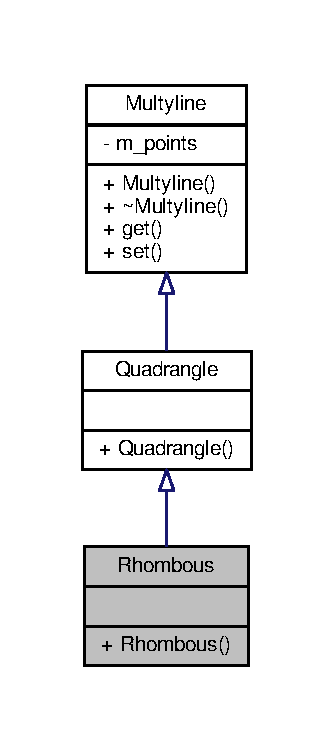
\includegraphics[width=160pt]{class_rhombous__inherit__graph}
\end{center}
\end{figure}


Граф связей класса Rhombous\-:
\nopagebreak
\begin{figure}[H]
\begin{center}
\leavevmode
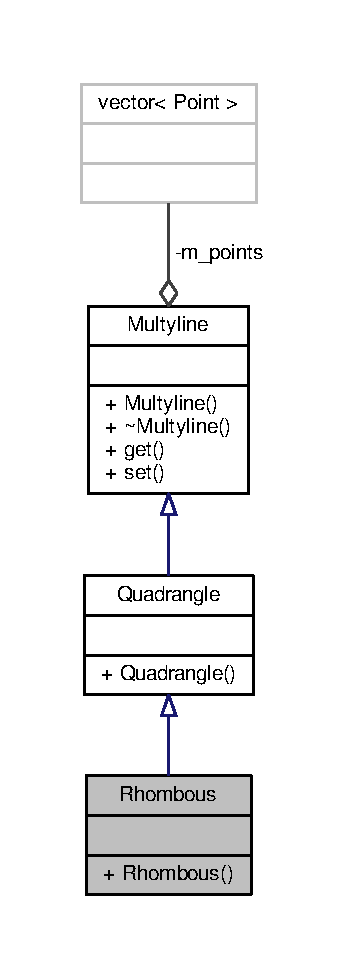
\includegraphics[width=167pt]{class_rhombous__coll__graph}
\end{center}
\end{figure}
\subsection*{Открытые типы}
\begin{DoxyCompactItemize}
\item 
enum \hyperlink{class_rhombous_ac90a281d31799c97af62a4b63a664058}{draw\-Method} \{ \hyperlink{class_rhombous_ac90a281d31799c97af62a4b63a664058a3afc60fab182c11851e7bb8870f77352}{point3}, 
\hyperlink{class_rhombous_ac90a281d31799c97af62a4b63a664058a16d219134eda7717ac1aa16061ece158}{point2}, 
\hyperlink{class_rhombous_ac90a281d31799c97af62a4b63a664058a28041197087f875dd594d5d04b4c43ab}{point1}
 \}
\end{DoxyCompactItemize}
\subsection*{Открытые члены}
\begin{DoxyCompactItemize}
\item 
\hyperlink{class_rhombous_a1abf251c711268cd2a8f7669f4bbc9a3}{Rhombous} (\hyperlink{class_multyline_ad75d7bb224267d0d7b4c40fd72a1d920}{draw\-Method}, std\-::initializer\-\_\-list$<$ double $>$ \&)
\end{DoxyCompactItemize}


\subsection{Подробное описание}


См. определение в файле m4\-\_\-basic.\-h строка 54



\subsection{Перечисления}
\hypertarget{class_rhombous_ac90a281d31799c97af62a4b63a664058}{\index{Rhombous@{Rhombous}!draw\-Method@{draw\-Method}}
\index{draw\-Method@{draw\-Method}!Rhombous@{Rhombous}}
\subsubsection[{draw\-Method}]{\setlength{\rightskip}{0pt plus 5cm}enum {\bf Rhombous\-::draw\-Method}}}\label{class_rhombous_ac90a281d31799c97af62a4b63a664058}
\begin{Desc}
\item[Элементы перечислений]\par
\begin{description}
\index{point3@{point3}!Rhombous@{Rhombous}}\index{Rhombous@{Rhombous}!point3@{point3}}\item[{\em 
\hypertarget{class_rhombous_ac90a281d31799c97af62a4b63a664058a3afc60fab182c11851e7bb8870f77352}{point3}\label{class_rhombous_ac90a281d31799c97af62a4b63a664058a3afc60fab182c11851e7bb8870f77352}
}]\index{point2@{point2}!Rhombous@{Rhombous}}\index{Rhombous@{Rhombous}!point2@{point2}}\item[{\em 
\hypertarget{class_rhombous_ac90a281d31799c97af62a4b63a664058a16d219134eda7717ac1aa16061ece158}{point2}\label{class_rhombous_ac90a281d31799c97af62a4b63a664058a16d219134eda7717ac1aa16061ece158}
}]\index{point1@{point1}!Rhombous@{Rhombous}}\index{Rhombous@{Rhombous}!point1@{point1}}\item[{\em 
\hypertarget{class_rhombous_ac90a281d31799c97af62a4b63a664058a28041197087f875dd594d5d04b4c43ab}{point1}\label{class_rhombous_ac90a281d31799c97af62a4b63a664058a28041197087f875dd594d5d04b4c43ab}
}]\end{description}
\end{Desc}


См. определение в файле m4\-\_\-basic.\-h строка 57



\subsection{Конструктор(ы)}
\hypertarget{class_rhombous_a1abf251c711268cd2a8f7669f4bbc9a3}{\index{Rhombous@{Rhombous}!Rhombous@{Rhombous}}
\index{Rhombous@{Rhombous}!Rhombous@{Rhombous}}
\subsubsection[{Rhombous}]{\setlength{\rightskip}{0pt plus 5cm}Rhombous\-::\-Rhombous (
\begin{DoxyParamCaption}
\item[{{\bf draw\-Method}}]{, }
\item[{std\-::initializer\-\_\-list$<$ double $>$ \&}]{}
\end{DoxyParamCaption}
)}}\label{class_rhombous_a1abf251c711268cd2a8f7669f4bbc9a3}


Объявления и описания членов класса находятся в файле\-:\begin{DoxyCompactItemize}
\item 
libs/models/m\-\_\-shapes/\hyperlink{m4__basic_8h}{m4\-\_\-basic.\-h}\end{DoxyCompactItemize}

\hypertarget{class_rhombous_controller}{\section{Класс Rhombous\-Controller}
\label{class_rhombous_controller}\index{Rhombous\-Controller@{Rhombous\-Controller}}
}


{\ttfamily \#include $<$base\-Controller.\-h$>$}



Граф наследования\-:Rhombous\-Controller\-:
\nopagebreak
\begin{figure}[H]
\begin{center}
\leavevmode
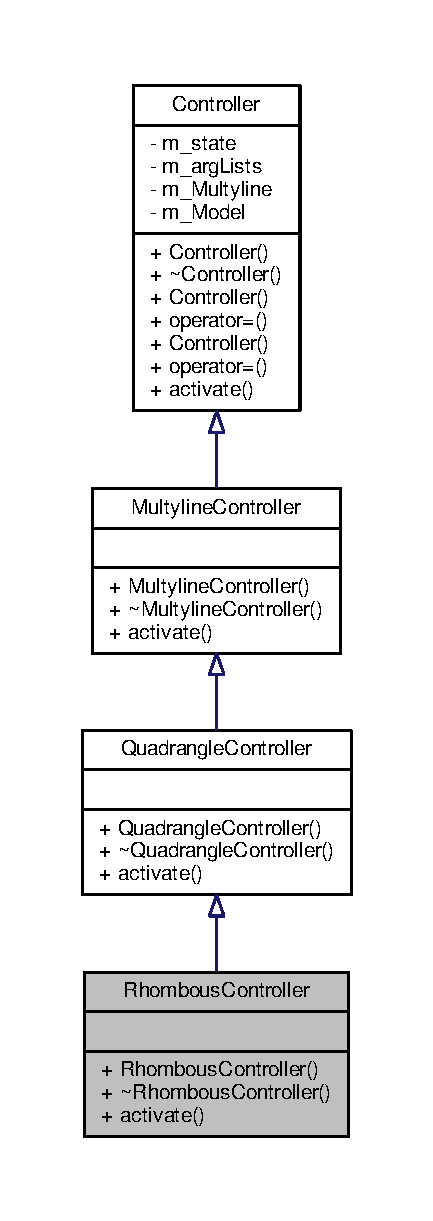
\includegraphics[height=550pt]{class_rhombous_controller__inherit__graph}
\end{center}
\end{figure}


Граф связей класса Rhombous\-Controller\-:
\nopagebreak
\begin{figure}[H]
\begin{center}
\leavevmode
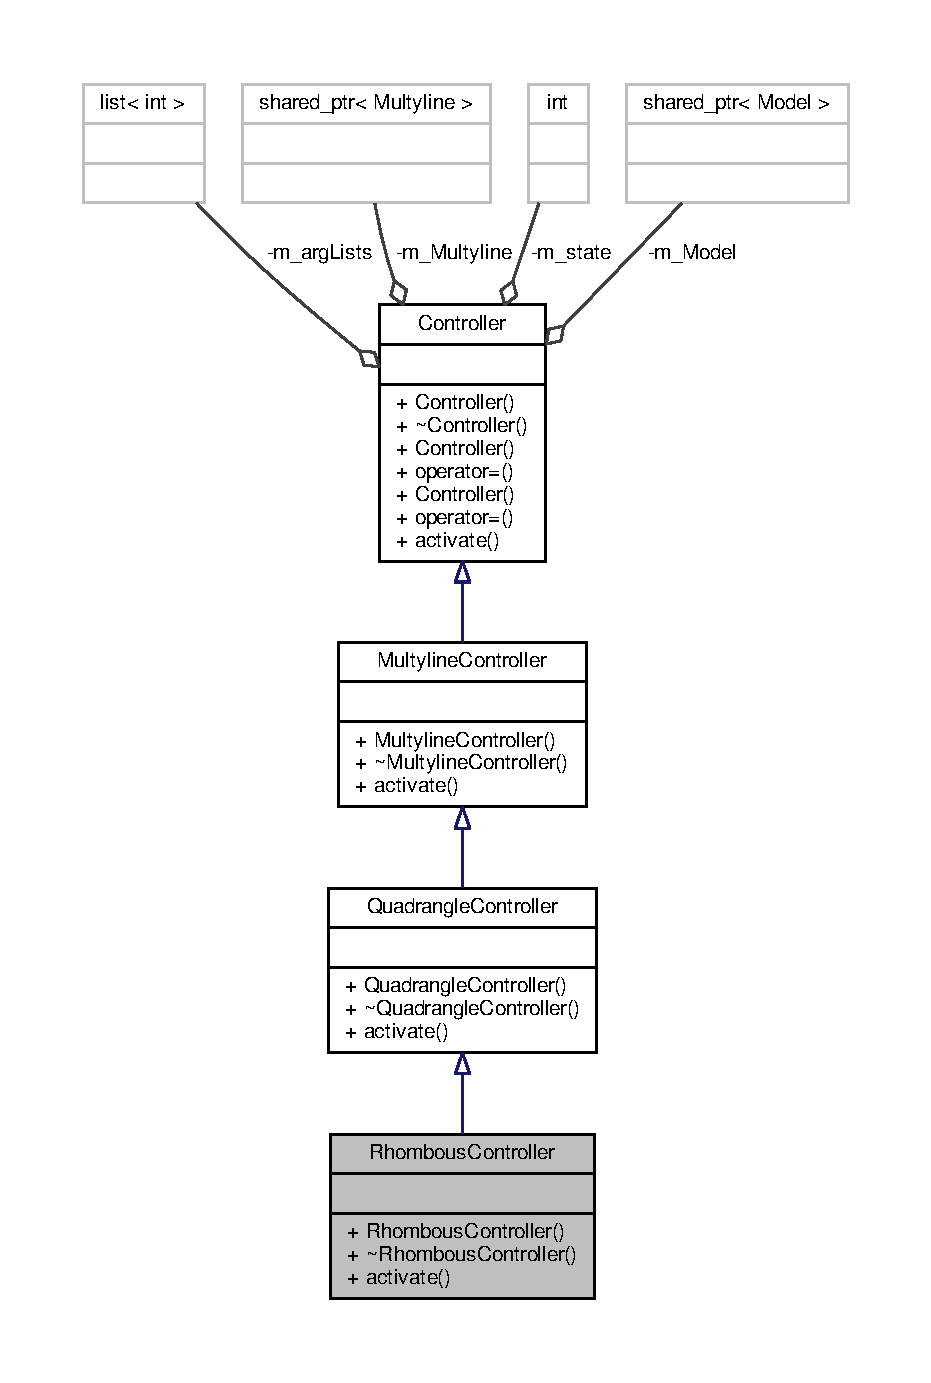
\includegraphics[width=350pt]{class_rhombous_controller__coll__graph}
\end{center}
\end{figure}
\subsection*{Открытые члены}
\begin{DoxyCompactItemize}
\item 
\hyperlink{class_rhombous_controller_af001407b5bd87b3bdedd7814d61184c0}{Rhombous\-Controller} (std\-::shared\-\_\-ptr$<$ \hyperlink{class_model}{Model} $>$ \&model)
\item 
\hyperlink{class_rhombous_controller_aa39b60d4b91fa169c71ae71a66fcc615}{$\sim$\-Rhombous\-Controller} ()=default
\item 
void \hyperlink{class_rhombous_controller_a9e839123b8a65d202fb898b6233694b2}{activate} (int cursor\-Pos\-X, int cursor\-Pos\-Y) final
\end{DoxyCompactItemize}


\subsection{Подробное описание}


См. определение в файле base\-Controller.\-h строка 211



\subsection{Конструктор(ы)}
\hypertarget{class_rhombous_controller_af001407b5bd87b3bdedd7814d61184c0}{\index{Rhombous\-Controller@{Rhombous\-Controller}!Rhombous\-Controller@{Rhombous\-Controller}}
\index{Rhombous\-Controller@{Rhombous\-Controller}!RhombousController@{Rhombous\-Controller}}
\subsubsection[{Rhombous\-Controller}]{\setlength{\rightskip}{0pt plus 5cm}Rhombous\-Controller\-::\-Rhombous\-Controller (
\begin{DoxyParamCaption}
\item[{std\-::shared\-\_\-ptr$<$ {\bf Model} $>$ \&}]{model}
\end{DoxyParamCaption}
)\hspace{0.3cm}{\ttfamily [inline]}}}\label{class_rhombous_controller_af001407b5bd87b3bdedd7814d61184c0}


См. определение в файле base\-Controller.\-h строка 214

\hypertarget{class_rhombous_controller_aa39b60d4b91fa169c71ae71a66fcc615}{\index{Rhombous\-Controller@{Rhombous\-Controller}!$\sim$\-Rhombous\-Controller@{$\sim$\-Rhombous\-Controller}}
\index{$\sim$\-Rhombous\-Controller@{$\sim$\-Rhombous\-Controller}!RhombousController@{Rhombous\-Controller}}
\subsubsection[{$\sim$\-Rhombous\-Controller}]{\setlength{\rightskip}{0pt plus 5cm}Rhombous\-Controller\-::$\sim$\-Rhombous\-Controller (
\begin{DoxyParamCaption}
{}
\end{DoxyParamCaption}
)\hspace{0.3cm}{\ttfamily [default]}}}\label{class_rhombous_controller_aa39b60d4b91fa169c71ae71a66fcc615}


\subsection{Методы}
\hypertarget{class_rhombous_controller_a9e839123b8a65d202fb898b6233694b2}{\index{Rhombous\-Controller@{Rhombous\-Controller}!activate@{activate}}
\index{activate@{activate}!RhombousController@{Rhombous\-Controller}}
\subsubsection[{activate}]{\setlength{\rightskip}{0pt plus 5cm}void Rhombous\-Controller\-::activate (
\begin{DoxyParamCaption}
\item[{int}]{cursor\-Pos\-X, }
\item[{int}]{cursor\-Pos\-Y}
\end{DoxyParamCaption}
)\hspace{0.3cm}{\ttfamily [inline]}, {\ttfamily [final]}, {\ttfamily [virtual]}}}\label{class_rhombous_controller_a9e839123b8a65d202fb898b6233694b2}


Переопределяет метод предка \hyperlink{class_quadrangle_controller_a2a38c3afba85014f27041e002cfc7950}{Quadrangle\-Controller}.



См. определение в файле base\-Controller.\-h строка 216



Объявления и описания членов класса находятся в файле\-:\begin{DoxyCompactItemize}
\item 
libs/controllers/\hyperlink{base_controller_8h}{base\-Controller.\-h}\end{DoxyCompactItemize}

\hypertarget{class_save_controller}{\section{Класс Save\-Controller}
\label{class_save_controller}\index{Save\-Controller@{Save\-Controller}}
}


{\ttfamily \#include $<$base\-Controller.\-h$>$}



Граф наследования\-:Save\-Controller\-:
\nopagebreak
\begin{figure}[H]
\begin{center}
\leavevmode
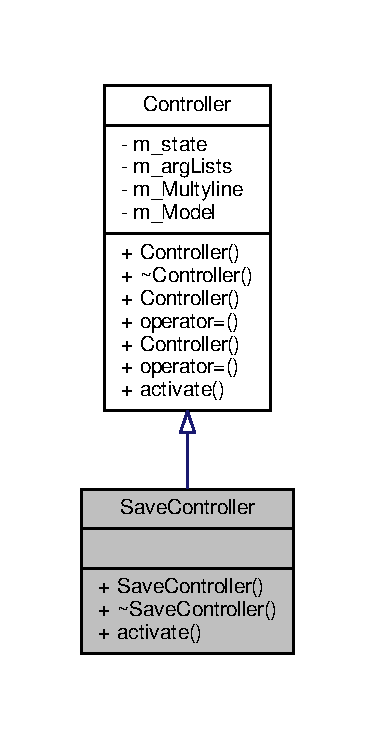
\includegraphics[width=180pt]{class_save_controller__inherit__graph}
\end{center}
\end{figure}


Граф связей класса Save\-Controller\-:
\nopagebreak
\begin{figure}[H]
\begin{center}
\leavevmode
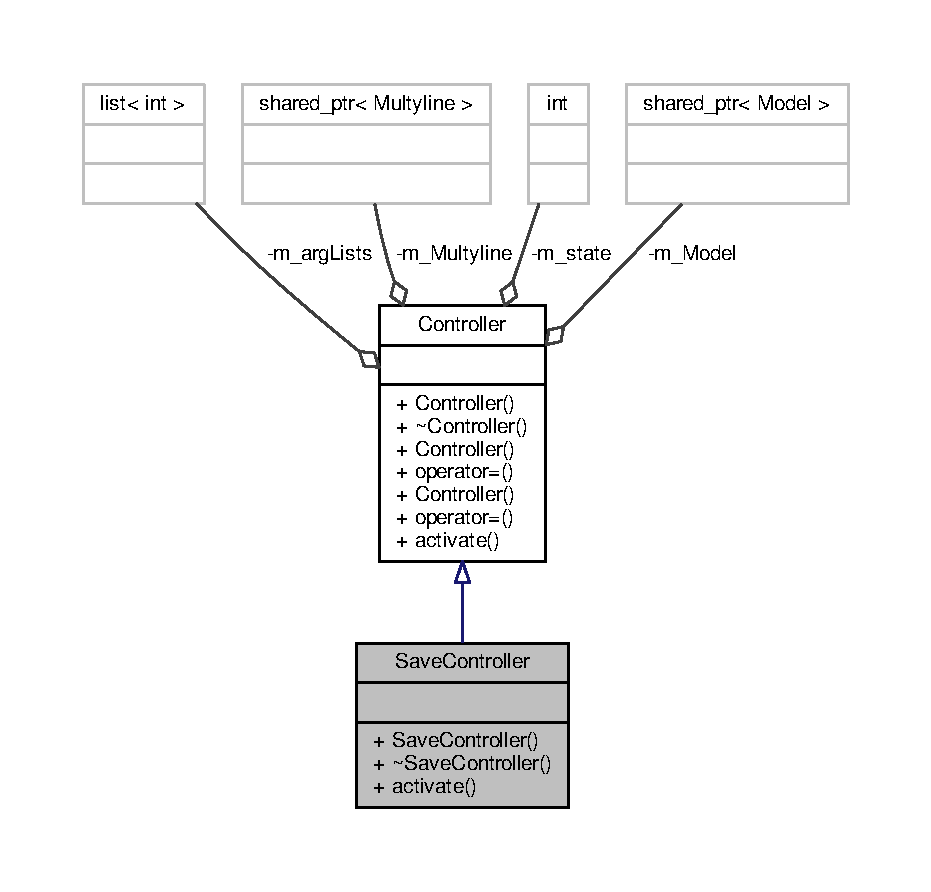
\includegraphics[width=350pt]{class_save_controller__coll__graph}
\end{center}
\end{figure}
\subsection*{Открытые члены}
\begin{DoxyCompactItemize}
\item 
\hyperlink{class_save_controller_aa8039a76832d89da06fbf5e63ba8c7e1}{Save\-Controller} (std\-::shared\-\_\-ptr$<$ \hyperlink{class_model}{Model} $>$ \&model)
\item 
\hyperlink{class_save_controller_ac4a37f1855232e795d306f1a8038c85b}{$\sim$\-Save\-Controller} ()=default
\item 
void \hyperlink{class_save_controller_a82d91ea99368d4cbce96a24d988a8c2b}{activate} (int cursor\-Pos\-X, int cursor\-Pos\-Y) final
\end{DoxyCompactItemize}


\subsection{Подробное описание}


См. определение в файле base\-Controller.\-h строка 61



\subsection{Конструктор(ы)}
\hypertarget{class_save_controller_aa8039a76832d89da06fbf5e63ba8c7e1}{\index{Save\-Controller@{Save\-Controller}!Save\-Controller@{Save\-Controller}}
\index{Save\-Controller@{Save\-Controller}!SaveController@{Save\-Controller}}
\subsubsection[{Save\-Controller}]{\setlength{\rightskip}{0pt plus 5cm}Save\-Controller\-::\-Save\-Controller (
\begin{DoxyParamCaption}
\item[{std\-::shared\-\_\-ptr$<$ {\bf Model} $>$ \&}]{model}
\end{DoxyParamCaption}
)\hspace{0.3cm}{\ttfamily [inline]}}}\label{class_save_controller_aa8039a76832d89da06fbf5e63ba8c7e1}


См. определение в файле base\-Controller.\-h строка 64

\hypertarget{class_save_controller_ac4a37f1855232e795d306f1a8038c85b}{\index{Save\-Controller@{Save\-Controller}!$\sim$\-Save\-Controller@{$\sim$\-Save\-Controller}}
\index{$\sim$\-Save\-Controller@{$\sim$\-Save\-Controller}!SaveController@{Save\-Controller}}
\subsubsection[{$\sim$\-Save\-Controller}]{\setlength{\rightskip}{0pt plus 5cm}Save\-Controller\-::$\sim$\-Save\-Controller (
\begin{DoxyParamCaption}
{}
\end{DoxyParamCaption}
)\hspace{0.3cm}{\ttfamily [default]}}}\label{class_save_controller_ac4a37f1855232e795d306f1a8038c85b}


\subsection{Методы}
\hypertarget{class_save_controller_a82d91ea99368d4cbce96a24d988a8c2b}{\index{Save\-Controller@{Save\-Controller}!activate@{activate}}
\index{activate@{activate}!SaveController@{Save\-Controller}}
\subsubsection[{activate}]{\setlength{\rightskip}{0pt plus 5cm}void Save\-Controller\-::activate (
\begin{DoxyParamCaption}
\item[{int}]{cursor\-Pos\-X, }
\item[{int}]{cursor\-Pos\-Y}
\end{DoxyParamCaption}
)\hspace{0.3cm}{\ttfamily [inline]}, {\ttfamily [final]}, {\ttfamily [virtual]}}}\label{class_save_controller_a82d91ea99368d4cbce96a24d988a8c2b}


Замещает \hyperlink{class_controller_a4cc69a630011f49efb0c221d617af633}{Controller}.



См. определение в файле base\-Controller.\-h строка 66



Объявления и описания членов класса находятся в файле\-:\begin{DoxyCompactItemize}
\item 
libs/controllers/\hyperlink{base_controller_8h}{base\-Controller.\-h}\end{DoxyCompactItemize}

\hypertarget{class_section}{\section{Класс Section}
\label{class_section}\index{Section@{Section}}
}


{\ttfamily \#include $<$m2\-\_\-section.\-h$>$}



Граф наследования\-:Section\-:
\nopagebreak
\begin{figure}[H]
\begin{center}
\leavevmode
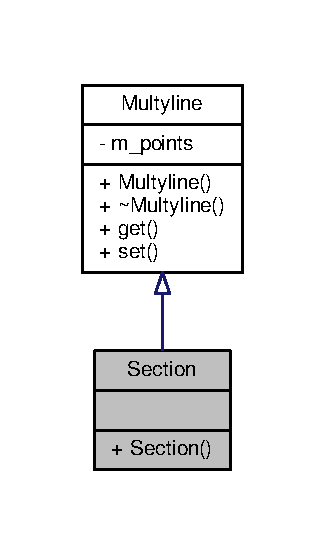
\includegraphics[width=156pt]{class_section__inherit__graph}
\end{center}
\end{figure}


Граф связей класса Section\-:
\nopagebreak
\begin{figure}[H]
\begin{center}
\leavevmode
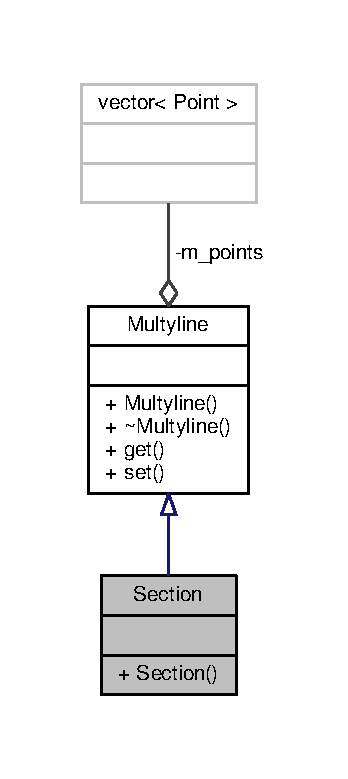
\includegraphics[width=167pt]{class_section__coll__graph}
\end{center}
\end{figure}
\subsection*{Открытые члены}
\begin{DoxyCompactItemize}
\item 
\hyperlink{class_section_a1a140cf180d250249215e06702a99162}{Section} (std\-::initializer\-\_\-list$<$ double $>$ \&points)
\end{DoxyCompactItemize}
\subsection*{Дополнительные унаследованные члены}


\subsection{Подробное описание}


См. определение в файле m2\-\_\-section.\-h строка 3



\subsection{Конструктор(ы)}
\hypertarget{class_section_a1a140cf180d250249215e06702a99162}{\index{Section@{Section}!Section@{Section}}
\index{Section@{Section}!Section@{Section}}
\subsubsection[{Section}]{\setlength{\rightskip}{0pt plus 5cm}Section\-::\-Section (
\begin{DoxyParamCaption}
\item[{std\-::initializer\-\_\-list$<$ double $>$ \&}]{points}
\end{DoxyParamCaption}
)\hspace{0.3cm}{\ttfamily [inline]}}}\label{class_section_a1a140cf180d250249215e06702a99162}


См. определение в файле m2\-\_\-section.\-h строка 6



Объявления и описания членов класса находятся в файле\-:\begin{DoxyCompactItemize}
\item 
libs/models/m\-\_\-shapes/\hyperlink{m2__section_8h}{m2\-\_\-section.\-h}\end{DoxyCompactItemize}

\hypertarget{class_section_controller}{\section{Класс Section\-Controller}
\label{class_section_controller}\index{Section\-Controller@{Section\-Controller}}
}


{\ttfamily \#include $<$base\-Controller.\-h$>$}



Граф наследования\-:Section\-Controller\-:
\nopagebreak
\begin{figure}[H]
\begin{center}
\leavevmode
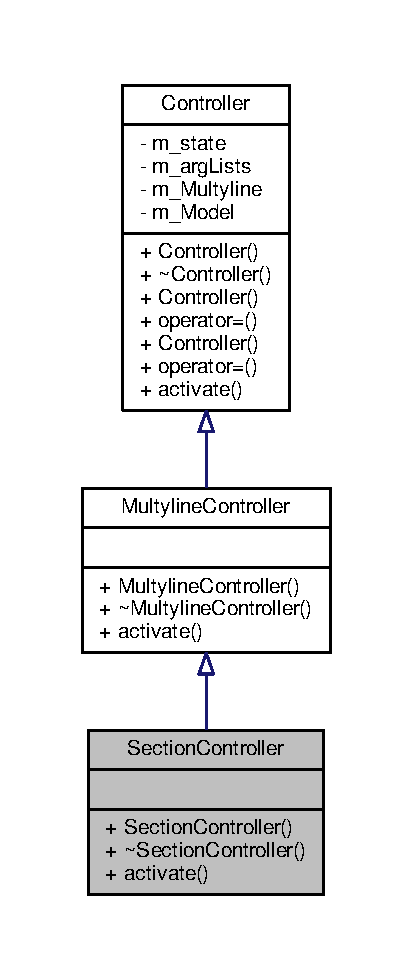
\includegraphics[width=198pt]{class_section_controller__inherit__graph}
\end{center}
\end{figure}


Граф связей класса Section\-Controller\-:
\nopagebreak
\begin{figure}[H]
\begin{center}
\leavevmode
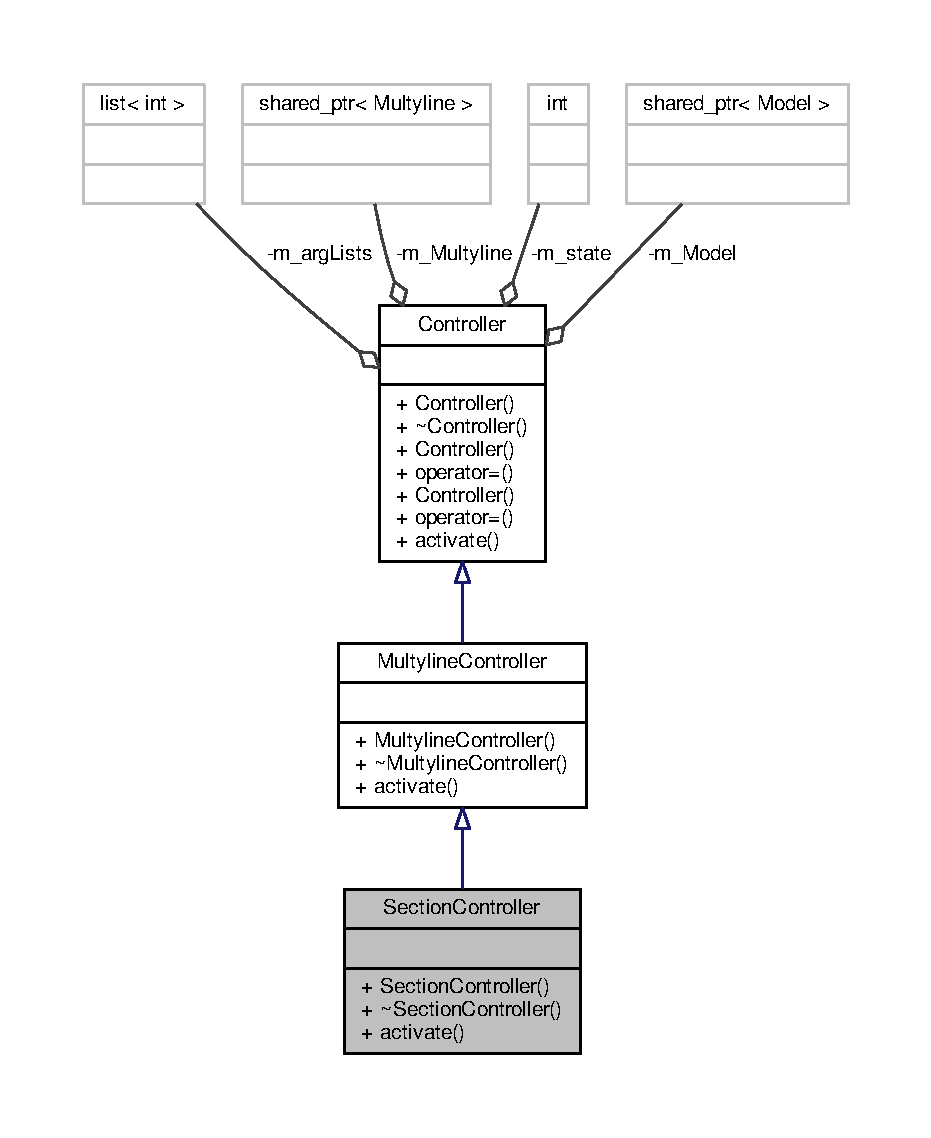
\includegraphics[width=350pt]{class_section_controller__coll__graph}
\end{center}
\end{figure}
\subsection*{Открытые члены}
\begin{DoxyCompactItemize}
\item 
\hyperlink{class_section_controller_a67316b2c4b0ca5c107108a9fa6104c99}{Section\-Controller} (std\-::shared\-\_\-ptr$<$ \hyperlink{class_model}{Model} $>$ \&model)
\item 
\hyperlink{class_section_controller_a33f3cd20b89d17016f066b47d03f9a47}{$\sim$\-Section\-Controller} ()=default
\item 
void \hyperlink{class_section_controller_ac42bb71f574f336a79a2e0a739fbad24}{activate} (int cursor\-Pos\-X, int cursor\-Pos\-Y) override
\end{DoxyCompactItemize}


\subsection{Подробное описание}


См. определение в файле base\-Controller.\-h строка 103



\subsection{Конструктор(ы)}
\hypertarget{class_section_controller_a67316b2c4b0ca5c107108a9fa6104c99}{\index{Section\-Controller@{Section\-Controller}!Section\-Controller@{Section\-Controller}}
\index{Section\-Controller@{Section\-Controller}!SectionController@{Section\-Controller}}
\subsubsection[{Section\-Controller}]{\setlength{\rightskip}{0pt plus 5cm}Section\-Controller\-::\-Section\-Controller (
\begin{DoxyParamCaption}
\item[{std\-::shared\-\_\-ptr$<$ {\bf Model} $>$ \&}]{model}
\end{DoxyParamCaption}
)\hspace{0.3cm}{\ttfamily [inline]}}}\label{class_section_controller_a67316b2c4b0ca5c107108a9fa6104c99}


См. определение в файле base\-Controller.\-h строка 106

\hypertarget{class_section_controller_a33f3cd20b89d17016f066b47d03f9a47}{\index{Section\-Controller@{Section\-Controller}!$\sim$\-Section\-Controller@{$\sim$\-Section\-Controller}}
\index{$\sim$\-Section\-Controller@{$\sim$\-Section\-Controller}!SectionController@{Section\-Controller}}
\subsubsection[{$\sim$\-Section\-Controller}]{\setlength{\rightskip}{0pt plus 5cm}Section\-Controller\-::$\sim$\-Section\-Controller (
\begin{DoxyParamCaption}
{}
\end{DoxyParamCaption}
)\hspace{0.3cm}{\ttfamily [default]}}}\label{class_section_controller_a33f3cd20b89d17016f066b47d03f9a47}


\subsection{Методы}
\hypertarget{class_section_controller_ac42bb71f574f336a79a2e0a739fbad24}{\index{Section\-Controller@{Section\-Controller}!activate@{activate}}
\index{activate@{activate}!SectionController@{Section\-Controller}}
\subsubsection[{activate}]{\setlength{\rightskip}{0pt plus 5cm}void Section\-Controller\-::activate (
\begin{DoxyParamCaption}
\item[{int}]{cursor\-Pos\-X, }
\item[{int}]{cursor\-Pos\-Y}
\end{DoxyParamCaption}
)\hspace{0.3cm}{\ttfamily [inline]}, {\ttfamily [override]}, {\ttfamily [virtual]}}}\label{class_section_controller_ac42bb71f574f336a79a2e0a739fbad24}


Переопределяет метод предка \hyperlink{class_multyline_controller_a5a574a5ca48d2a7e62201e9415a61afe}{Multyline\-Controller}.



См. определение в файле base\-Controller.\-h строка 108



Объявления и описания членов класса находятся в файле\-:\begin{DoxyCompactItemize}
\item 
libs/controllers/\hyperlink{base_controller_8h}{base\-Controller.\-h}\end{DoxyCompactItemize}

\hypertarget{class_square}{\section{Класс Square}
\label{class_square}\index{Square@{Square}}
}


{\ttfamily \#include $<$m4\-\_\-basic.\-h$>$}



Граф наследования\-:Square\-:
\nopagebreak
\begin{figure}[H]
\begin{center}
\leavevmode
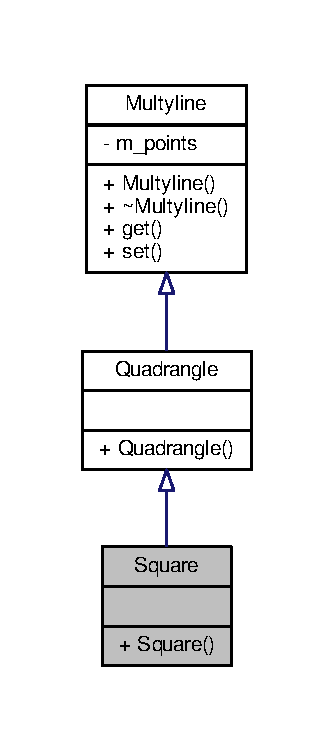
\includegraphics[width=160pt]{class_square__inherit__graph}
\end{center}
\end{figure}


Граф связей класса Square\-:
\nopagebreak
\begin{figure}[H]
\begin{center}
\leavevmode
\includegraphics[width=167pt]{class_square__coll__graph}
\end{center}
\end{figure}
\subsection*{Открытые типы}
\begin{DoxyCompactItemize}
\item 
enum \hyperlink{class_square_afb936005821ce22a9ecfbd2b3a0cfb13}{draw\-Method} \{ \hyperlink{class_square_afb936005821ce22a9ecfbd2b3a0cfb13aaf7215e74b713a4de0eeda3912b2eb82}{side}, 
\hyperlink{class_square_afb936005821ce22a9ecfbd2b3a0cfb13a52ec280a7edeecdef1ebc0439b83e5ac}{diagonal}
 \}
\end{DoxyCompactItemize}
\subsection*{Открытые члены}
\begin{DoxyCompactItemize}
\item 
\hyperlink{class_square_adf29bfeb59b78ed77afef908a3bc2745}{Square} (\hyperlink{class_multyline_ad75d7bb224267d0d7b4c40fd72a1d920}{draw\-Method}, std\-::initializer\-\_\-list$<$ double $>$ \&)
\end{DoxyCompactItemize}


\subsection{Подробное описание}


См. определение в файле m4\-\_\-basic.\-h строка 19



\subsection{Перечисления}
\hypertarget{class_square_afb936005821ce22a9ecfbd2b3a0cfb13}{\index{Square@{Square}!draw\-Method@{draw\-Method}}
\index{draw\-Method@{draw\-Method}!Square@{Square}}
\subsubsection[{draw\-Method}]{\setlength{\rightskip}{0pt plus 5cm}enum {\bf Square\-::draw\-Method}}}\label{class_square_afb936005821ce22a9ecfbd2b3a0cfb13}
\begin{Desc}
\item[Элементы перечислений]\par
\begin{description}
\index{side@{side}!Square@{Square}}\index{Square@{Square}!side@{side}}\item[{\em 
\hypertarget{class_square_afb936005821ce22a9ecfbd2b3a0cfb13aaf7215e74b713a4de0eeda3912b2eb82}{side}\label{class_square_afb936005821ce22a9ecfbd2b3a0cfb13aaf7215e74b713a4de0eeda3912b2eb82}
}]\index{diagonal@{diagonal}!Square@{Square}}\index{Square@{Square}!diagonal@{diagonal}}\item[{\em 
\hypertarget{class_square_afb936005821ce22a9ecfbd2b3a0cfb13a52ec280a7edeecdef1ebc0439b83e5ac}{diagonal}\label{class_square_afb936005821ce22a9ecfbd2b3a0cfb13a52ec280a7edeecdef1ebc0439b83e5ac}
}]\end{description}
\end{Desc}


См. определение в файле m4\-\_\-basic.\-h строка 22



\subsection{Конструктор(ы)}
\hypertarget{class_square_adf29bfeb59b78ed77afef908a3bc2745}{\index{Square@{Square}!Square@{Square}}
\index{Square@{Square}!Square@{Square}}
\subsubsection[{Square}]{\setlength{\rightskip}{0pt plus 5cm}Square\-::\-Square (
\begin{DoxyParamCaption}
\item[{{\bf draw\-Method}}]{, }
\item[{std\-::initializer\-\_\-list$<$ double $>$ \&}]{}
\end{DoxyParamCaption}
)}}\label{class_square_adf29bfeb59b78ed77afef908a3bc2745}


Объявления и описания членов класса находятся в файле\-:\begin{DoxyCompactItemize}
\item 
libs/models/m\-\_\-shapes/\hyperlink{m4__basic_8h}{m4\-\_\-basic.\-h}\end{DoxyCompactItemize}

\hypertarget{class_square_controller}{\section{Класс Square\-Controller}
\label{class_square_controller}\index{Square\-Controller@{Square\-Controller}}
}


{\ttfamily \#include $<$base\-Controller.\-h$>$}



Граф наследования\-:Square\-Controller\-:
\nopagebreak
\begin{figure}[H]
\begin{center}
\leavevmode
\includegraphics[height=550pt]{class_square_controller__inherit__graph}
\end{center}
\end{figure}


Граф связей класса Square\-Controller\-:
\nopagebreak
\begin{figure}[H]
\begin{center}
\leavevmode
\includegraphics[width=350pt]{class_square_controller__coll__graph}
\end{center}
\end{figure}
\subsection*{Открытые члены}
\begin{DoxyCompactItemize}
\item 
\hyperlink{class_square_controller_a64d29b2a5ba3fc6dfe1d9402d32e552a}{Square\-Controller} (std\-::shared\-\_\-ptr$<$ \hyperlink{class_model}{Model} $>$ \&model)
\item 
virtual \hyperlink{class_square_controller_aaac778e973aa3419f0a3dacaed16bdc5}{$\sim$\-Square\-Controller} ()=default
\item 
void \hyperlink{class_square_controller_a169d59d75dd023ed352e7722a3bd2dcc}{activate} (int cursor\-Pos\-X, int cursor\-Pos\-Y) final
\end{DoxyCompactItemize}


\subsection{Подробное описание}


См. определение в файле base\-Controller.\-h строка 185



\subsection{Конструктор(ы)}
\hypertarget{class_square_controller_a64d29b2a5ba3fc6dfe1d9402d32e552a}{\index{Square\-Controller@{Square\-Controller}!Square\-Controller@{Square\-Controller}}
\index{Square\-Controller@{Square\-Controller}!SquareController@{Square\-Controller}}
\subsubsection[{Square\-Controller}]{\setlength{\rightskip}{0pt plus 5cm}Square\-Controller\-::\-Square\-Controller (
\begin{DoxyParamCaption}
\item[{std\-::shared\-\_\-ptr$<$ {\bf Model} $>$ \&}]{model}
\end{DoxyParamCaption}
)\hspace{0.3cm}{\ttfamily [inline]}}}\label{class_square_controller_a64d29b2a5ba3fc6dfe1d9402d32e552a}


См. определение в файле base\-Controller.\-h строка 188

\hypertarget{class_square_controller_aaac778e973aa3419f0a3dacaed16bdc5}{\index{Square\-Controller@{Square\-Controller}!$\sim$\-Square\-Controller@{$\sim$\-Square\-Controller}}
\index{$\sim$\-Square\-Controller@{$\sim$\-Square\-Controller}!SquareController@{Square\-Controller}}
\subsubsection[{$\sim$\-Square\-Controller}]{\setlength{\rightskip}{0pt plus 5cm}virtual Square\-Controller\-::$\sim$\-Square\-Controller (
\begin{DoxyParamCaption}
{}
\end{DoxyParamCaption}
)\hspace{0.3cm}{\ttfamily [virtual]}, {\ttfamily [default]}}}\label{class_square_controller_aaac778e973aa3419f0a3dacaed16bdc5}


\subsection{Методы}
\hypertarget{class_square_controller_a169d59d75dd023ed352e7722a3bd2dcc}{\index{Square\-Controller@{Square\-Controller}!activate@{activate}}
\index{activate@{activate}!SquareController@{Square\-Controller}}
\subsubsection[{activate}]{\setlength{\rightskip}{0pt plus 5cm}void Square\-Controller\-::activate (
\begin{DoxyParamCaption}
\item[{int}]{cursor\-Pos\-X, }
\item[{int}]{cursor\-Pos\-Y}
\end{DoxyParamCaption}
)\hspace{0.3cm}{\ttfamily [inline]}, {\ttfamily [final]}, {\ttfamily [virtual]}}}\label{class_square_controller_a169d59d75dd023ed352e7722a3bd2dcc}


Переопределяет метод предка \hyperlink{class_quadrangle_controller_a2a38c3afba85014f27041e002cfc7950}{Quadrangle\-Controller}.



См. определение в файле base\-Controller.\-h строка 190



Объявления и описания членов класса находятся в файле\-:\begin{DoxyCompactItemize}
\item 
libs/controllers/\hyperlink{base_controller_8h}{base\-Controller.\-h}\end{DoxyCompactItemize}

\hypertarget{class_triangle}{\section{Класс Triangle}
\label{class_triangle}\index{Triangle@{Triangle}}
}


{\ttfamily \#include $<$m3\-\_\-basic.\-h$>$}



Граф наследования\-:Triangle\-:
\nopagebreak
\begin{figure}[H]
\begin{center}
\leavevmode
\includegraphics[width=350pt]{class_triangle__inherit__graph}
\end{center}
\end{figure}


Граф связей класса Triangle\-:
\nopagebreak
\begin{figure}[H]
\begin{center}
\leavevmode
\includegraphics[width=167pt]{class_triangle__coll__graph}
\end{center}
\end{figure}
\subsection*{Открытые члены}
\begin{DoxyCompactItemize}
\item 
\hyperlink{class_triangle_a2487fe242d63ec49a77d522906d8f7ca}{Triangle} (std\-::initializer\-\_\-list$<$ double $>$ \&points)
\end{DoxyCompactItemize}
\subsection*{Дополнительные унаследованные члены}


\subsection{Подробное описание}


См. определение в файле m3\-\_\-basic.\-h строка 6



\subsection{Конструктор(ы)}
\hypertarget{class_triangle_a2487fe242d63ec49a77d522906d8f7ca}{\index{Triangle@{Triangle}!Triangle@{Triangle}}
\index{Triangle@{Triangle}!Triangle@{Triangle}}
\subsubsection[{Triangle}]{\setlength{\rightskip}{0pt plus 5cm}Triangle\-::\-Triangle (
\begin{DoxyParamCaption}
\item[{std\-::initializer\-\_\-list$<$ double $>$ \&}]{points}
\end{DoxyParamCaption}
)\hspace{0.3cm}{\ttfamily [inline]}}}\label{class_triangle_a2487fe242d63ec49a77d522906d8f7ca}


См. определение в файле m3\-\_\-basic.\-h строка 9



Объявления и описания членов класса находятся в файле\-:\begin{DoxyCompactItemize}
\item 
libs/models/m\-\_\-shapes/\hyperlink{m3__basic_8h}{m3\-\_\-basic.\-h}\end{DoxyCompactItemize}

\hypertarget{class_triangle_controller}{\section{Класс Triangle\-Controller}
\label{class_triangle_controller}\index{Triangle\-Controller@{Triangle\-Controller}}
}


{\ttfamily \#include $<$base\-Controller.\-h$>$}



Граф наследования\-:Triangle\-Controller\-:
\nopagebreak
\begin{figure}[H]
\begin{center}
\leavevmode
\includegraphics[width=350pt]{class_triangle_controller__inherit__graph}
\end{center}
\end{figure}


Граф связей класса Triangle\-Controller\-:
\nopagebreak
\begin{figure}[H]
\begin{center}
\leavevmode
\includegraphics[width=350pt]{class_triangle_controller__coll__graph}
\end{center}
\end{figure}
\subsection*{Открытые члены}
\begin{DoxyCompactItemize}
\item 
\hyperlink{class_triangle_controller_ad6c09eeb592bdd4f9afab1aea1d26921}{Triangle\-Controller} (std\-::shared\-\_\-ptr$<$ \hyperlink{class_model}{Model} $>$ \&model)
\item 
virtual \hyperlink{class_triangle_controller_a5eafaed903ec96ae942bf36cfa5c05d4}{$\sim$\-Triangle\-Controller} ()=default
\item 
void \hyperlink{class_triangle_controller_ab86471e4de39ae99bc6198583d173c7b}{activate} (int cursor\-Pos\-X, int cursor\-Pos\-Y) override
\end{DoxyCompactItemize}


\subsection{Подробное описание}


См. определение в файле base\-Controller.\-h строка 118



\subsection{Конструктор(ы)}
\hypertarget{class_triangle_controller_ad6c09eeb592bdd4f9afab1aea1d26921}{\index{Triangle\-Controller@{Triangle\-Controller}!Triangle\-Controller@{Triangle\-Controller}}
\index{Triangle\-Controller@{Triangle\-Controller}!TriangleController@{Triangle\-Controller}}
\subsubsection[{Triangle\-Controller}]{\setlength{\rightskip}{0pt plus 5cm}Triangle\-Controller\-::\-Triangle\-Controller (
\begin{DoxyParamCaption}
\item[{std\-::shared\-\_\-ptr$<$ {\bf Model} $>$ \&}]{model}
\end{DoxyParamCaption}
)\hspace{0.3cm}{\ttfamily [inline]}}}\label{class_triangle_controller_ad6c09eeb592bdd4f9afab1aea1d26921}


См. определение в файле base\-Controller.\-h строка 121

\hypertarget{class_triangle_controller_a5eafaed903ec96ae942bf36cfa5c05d4}{\index{Triangle\-Controller@{Triangle\-Controller}!$\sim$\-Triangle\-Controller@{$\sim$\-Triangle\-Controller}}
\index{$\sim$\-Triangle\-Controller@{$\sim$\-Triangle\-Controller}!TriangleController@{Triangle\-Controller}}
\subsubsection[{$\sim$\-Triangle\-Controller}]{\setlength{\rightskip}{0pt plus 5cm}virtual Triangle\-Controller\-::$\sim$\-Triangle\-Controller (
\begin{DoxyParamCaption}
{}
\end{DoxyParamCaption}
)\hspace{0.3cm}{\ttfamily [virtual]}, {\ttfamily [default]}}}\label{class_triangle_controller_a5eafaed903ec96ae942bf36cfa5c05d4}


\subsection{Методы}
\hypertarget{class_triangle_controller_ab86471e4de39ae99bc6198583d173c7b}{\index{Triangle\-Controller@{Triangle\-Controller}!activate@{activate}}
\index{activate@{activate}!TriangleController@{Triangle\-Controller}}
\subsubsection[{activate}]{\setlength{\rightskip}{0pt plus 5cm}void Triangle\-Controller\-::activate (
\begin{DoxyParamCaption}
\item[{int}]{cursor\-Pos\-X, }
\item[{int}]{cursor\-Pos\-Y}
\end{DoxyParamCaption}
)\hspace{0.3cm}{\ttfamily [inline]}, {\ttfamily [override]}, {\ttfamily [virtual]}}}\label{class_triangle_controller_ab86471e4de39ae99bc6198583d173c7b}


Переопределяет метод предка \hyperlink{class_multyline_controller_a5a574a5ca48d2a7e62201e9415a61afe}{Multyline\-Controller}.



Переопределяется в \hyperlink{class_equilateral_triangle_controller_ac8822ad6419def097652fc8a88426898}{Equilateral\-Triangle\-Controller}, \hyperlink{class_isosceles_triangle_controller_ac060b7bdfdc3c5fc078147e14e31415b}{Isosceles\-Triangle\-Controller} и \hyperlink{class_versatile_triangle_controller_a0d553f2393114a789f3e3964b97dad66}{Versatile\-Triangle\-Controller}.



См. определение в файле base\-Controller.\-h строка 123



Объявления и описания членов класса находятся в файле\-:\begin{DoxyCompactItemize}
\item 
libs/controllers/\hyperlink{base_controller_8h}{base\-Controller.\-h}\end{DoxyCompactItemize}

\hypertarget{class_versatile_quadrangle}{\section{Класс Versatile\-Quadrangle}
\label{class_versatile_quadrangle}\index{Versatile\-Quadrangle@{Versatile\-Quadrangle}}
}


{\ttfamily \#include $<$m4\-\_\-basic.\-h$>$}



Граф наследования\-:Versatile\-Quadrangle\-:
\nopagebreak
\begin{figure}[H]
\begin{center}
\leavevmode
\includegraphics[width=198pt]{class_versatile_quadrangle__inherit__graph}
\end{center}
\end{figure}


Граф связей класса Versatile\-Quadrangle\-:
\nopagebreak
\begin{figure}[H]
\begin{center}
\leavevmode
\includegraphics[width=198pt]{class_versatile_quadrangle__coll__graph}
\end{center}
\end{figure}
\subsection*{Открытые типы}
\begin{DoxyCompactItemize}
\item 
enum \hyperlink{class_versatile_quadrangle_aa897c08c7c9faf1813e7df4194a71e37}{draw\-Method} \{ \hyperlink{class_versatile_quadrangle_aa897c08c7c9faf1813e7df4194a71e37aaae92cad588cdacc57f810f244da32e0}{point4}
 \}
\end{DoxyCompactItemize}
\subsection*{Открытые члены}
\begin{DoxyCompactItemize}
\item 
\hyperlink{class_versatile_quadrangle_a5740f0b17fdca9d9de0dfe52e58412ea}{Versatile\-Quadrangle} (\hyperlink{class_multyline_ad75d7bb224267d0d7b4c40fd72a1d920}{draw\-Method}, std\-::initializer\-\_\-list$<$ double $>$ \&)
\end{DoxyCompactItemize}


\subsection{Подробное описание}


См. определение в файле m4\-\_\-basic.\-h строка 88



\subsection{Перечисления}
\hypertarget{class_versatile_quadrangle_aa897c08c7c9faf1813e7df4194a71e37}{\index{Versatile\-Quadrangle@{Versatile\-Quadrangle}!draw\-Method@{draw\-Method}}
\index{draw\-Method@{draw\-Method}!VersatileQuadrangle@{Versatile\-Quadrangle}}
\subsubsection[{draw\-Method}]{\setlength{\rightskip}{0pt plus 5cm}enum {\bf Versatile\-Quadrangle\-::draw\-Method}}}\label{class_versatile_quadrangle_aa897c08c7c9faf1813e7df4194a71e37}
\begin{Desc}
\item[Элементы перечислений]\par
\begin{description}
\index{point4@{point4}!Versatile\-Quadrangle@{Versatile\-Quadrangle}}\index{Versatile\-Quadrangle@{Versatile\-Quadrangle}!point4@{point4}}\item[{\em 
\hypertarget{class_versatile_quadrangle_aa897c08c7c9faf1813e7df4194a71e37aaae92cad588cdacc57f810f244da32e0}{point4}\label{class_versatile_quadrangle_aa897c08c7c9faf1813e7df4194a71e37aaae92cad588cdacc57f810f244da32e0}
}]\end{description}
\end{Desc}


См. определение в файле m4\-\_\-basic.\-h строка 91



\subsection{Конструктор(ы)}
\hypertarget{class_versatile_quadrangle_a5740f0b17fdca9d9de0dfe52e58412ea}{\index{Versatile\-Quadrangle@{Versatile\-Quadrangle}!Versatile\-Quadrangle@{Versatile\-Quadrangle}}
\index{Versatile\-Quadrangle@{Versatile\-Quadrangle}!VersatileQuadrangle@{Versatile\-Quadrangle}}
\subsubsection[{Versatile\-Quadrangle}]{\setlength{\rightskip}{0pt plus 5cm}Versatile\-Quadrangle\-::\-Versatile\-Quadrangle (
\begin{DoxyParamCaption}
\item[{{\bf draw\-Method}}]{, }
\item[{std\-::initializer\-\_\-list$<$ double $>$ \&}]{}
\end{DoxyParamCaption}
)}}\label{class_versatile_quadrangle_a5740f0b17fdca9d9de0dfe52e58412ea}


Объявления и описания членов класса находятся в файле\-:\begin{DoxyCompactItemize}
\item 
libs/models/m\-\_\-shapes/\hyperlink{m4__basic_8h}{m4\-\_\-basic.\-h}\end{DoxyCompactItemize}

\hypertarget{class_versatile_triangle}{\section{Класс Versatile\-Triangle}
\label{class_versatile_triangle}\index{Versatile\-Triangle@{Versatile\-Triangle}}
}


{\ttfamily \#include $<$m3\-\_\-basic.\-h$>$}



Граф наследования\-:Versatile\-Triangle\-:
\nopagebreak
\begin{figure}[H]
\begin{center}
\leavevmode
\includegraphics[width=180pt]{class_versatile_triangle__inherit__graph}
\end{center}
\end{figure}


Граф связей класса Versatile\-Triangle\-:
\nopagebreak
\begin{figure}[H]
\begin{center}
\leavevmode
\includegraphics[width=180pt]{class_versatile_triangle__coll__graph}
\end{center}
\end{figure}
\subsection*{Закрытые типы}
\begin{DoxyCompactItemize}
\item 
enum \hyperlink{class_versatile_triangle_ac4d324c8cbe82814fe769899adfc8678}{draw\-Method} \{ \hyperlink{class_versatile_triangle_ac4d324c8cbe82814fe769899adfc8678ab3b58d2ea402d320ea64301bc1af59e3}{point1}, 
\hyperlink{class_versatile_triangle_ac4d324c8cbe82814fe769899adfc8678abf098998afad6663f3e41cba9cbca69e}{point2}, 
\hyperlink{class_versatile_triangle_ac4d324c8cbe82814fe769899adfc8678ad47b6fee6cca0e5c5a42d2baf3a81e2b}{point3}
 \}
\end{DoxyCompactItemize}
\subsection*{Закрытые члены}
\begin{DoxyCompactItemize}
\item 
\hyperlink{class_versatile_triangle_aab319a2dd10de4db6eae4adae03e9621}{Versatile\-Triangle} (\hyperlink{class_multyline_ad75d7bb224267d0d7b4c40fd72a1d920}{draw\-Method}, std\-::initializer\-\_\-list$<$ double $>$ \&)
\end{DoxyCompactItemize}
\subsection*{Дополнительные унаследованные члены}


\subsection{Подробное описание}


См. определение в файле m3\-\_\-basic.\-h строка 20



\subsection{Перечисления}
\hypertarget{class_versatile_triangle_ac4d324c8cbe82814fe769899adfc8678}{\index{Versatile\-Triangle@{Versatile\-Triangle}!draw\-Method@{draw\-Method}}
\index{draw\-Method@{draw\-Method}!VersatileTriangle@{Versatile\-Triangle}}
\subsubsection[{draw\-Method}]{\setlength{\rightskip}{0pt plus 5cm}enum {\bf Versatile\-Triangle\-::draw\-Method}\hspace{0.3cm}{\ttfamily [private]}}}\label{class_versatile_triangle_ac4d324c8cbe82814fe769899adfc8678}
\begin{Desc}
\item[Элементы перечислений]\par
\begin{description}
\index{point1@{point1}!Versatile\-Triangle@{Versatile\-Triangle}}\index{Versatile\-Triangle@{Versatile\-Triangle}!point1@{point1}}\item[{\em 
\hypertarget{class_versatile_triangle_ac4d324c8cbe82814fe769899adfc8678ab3b58d2ea402d320ea64301bc1af59e3}{point1}\label{class_versatile_triangle_ac4d324c8cbe82814fe769899adfc8678ab3b58d2ea402d320ea64301bc1af59e3}
}]\index{point2@{point2}!Versatile\-Triangle@{Versatile\-Triangle}}\index{Versatile\-Triangle@{Versatile\-Triangle}!point2@{point2}}\item[{\em 
\hypertarget{class_versatile_triangle_ac4d324c8cbe82814fe769899adfc8678abf098998afad6663f3e41cba9cbca69e}{point2}\label{class_versatile_triangle_ac4d324c8cbe82814fe769899adfc8678abf098998afad6663f3e41cba9cbca69e}
}]\index{point3@{point3}!Versatile\-Triangle@{Versatile\-Triangle}}\index{Versatile\-Triangle@{Versatile\-Triangle}!point3@{point3}}\item[{\em 
\hypertarget{class_versatile_triangle_ac4d324c8cbe82814fe769899adfc8678ad47b6fee6cca0e5c5a42d2baf3a81e2b}{point3}\label{class_versatile_triangle_ac4d324c8cbe82814fe769899adfc8678ad47b6fee6cca0e5c5a42d2baf3a81e2b}
}]\end{description}
\end{Desc}


См. определение в файле m3\-\_\-basic.\-h строка 22



\subsection{Конструктор(ы)}
\hypertarget{class_versatile_triangle_aab319a2dd10de4db6eae4adae03e9621}{\index{Versatile\-Triangle@{Versatile\-Triangle}!Versatile\-Triangle@{Versatile\-Triangle}}
\index{Versatile\-Triangle@{Versatile\-Triangle}!VersatileTriangle@{Versatile\-Triangle}}
\subsubsection[{Versatile\-Triangle}]{\setlength{\rightskip}{0pt plus 5cm}Versatile\-Triangle\-::\-Versatile\-Triangle (
\begin{DoxyParamCaption}
\item[{{\bf draw\-Method}}]{, }
\item[{std\-::initializer\-\_\-list$<$ double $>$ \&}]{}
\end{DoxyParamCaption}
)\hspace{0.3cm}{\ttfamily [private]}}}\label{class_versatile_triangle_aab319a2dd10de4db6eae4adae03e9621}


Объявления и описания членов класса находятся в файле\-:\begin{DoxyCompactItemize}
\item 
libs/models/m\-\_\-shapes/\hyperlink{m3__basic_8h}{m3\-\_\-basic.\-h}\end{DoxyCompactItemize}

\hypertarget{class_versatile_triangle_controller}{\section{Класс Versatile\-Triangle\-Controller}
\label{class_versatile_triangle_controller}\index{Versatile\-Triangle\-Controller@{Versatile\-Triangle\-Controller}}
}


{\ttfamily \#include $<$base\-Controller.\-h$>$}



Граф наследования\-:Versatile\-Triangle\-Controller\-:
\nopagebreak
\begin{figure}[H]
\begin{center}
\leavevmode
\includegraphics[height=550pt]{class_versatile_triangle_controller__inherit__graph}
\end{center}
\end{figure}


Граф связей класса Versatile\-Triangle\-Controller\-:
\nopagebreak
\begin{figure}[H]
\begin{center}
\leavevmode
\includegraphics[width=350pt]{class_versatile_triangle_controller__coll__graph}
\end{center}
\end{figure}
\subsection*{Открытые члены}
\begin{DoxyCompactItemize}
\item 
\hyperlink{class_versatile_triangle_controller_a56d71d54f87562a6bef7978293e681e1}{Versatile\-Triangle\-Controller} (std\-::shared\-\_\-ptr$<$ \hyperlink{class_model}{Model} $>$ \&model)
\item 
\hyperlink{class_versatile_triangle_controller_aed1703ed1565b8693a896e044be4475e}{$\sim$\-Versatile\-Triangle\-Controller} ()=default
\item 
void \hyperlink{class_versatile_triangle_controller_a0d553f2393114a789f3e3964b97dad66}{activate} (int cursor\-Pos\-X, int cursor\-Pos\-Y) final
\end{DoxyCompactItemize}


\subsection{Подробное описание}


См. определение в файле base\-Controller.\-h строка 131



\subsection{Конструктор(ы)}
\hypertarget{class_versatile_triangle_controller_a56d71d54f87562a6bef7978293e681e1}{\index{Versatile\-Triangle\-Controller@{Versatile\-Triangle\-Controller}!Versatile\-Triangle\-Controller@{Versatile\-Triangle\-Controller}}
\index{Versatile\-Triangle\-Controller@{Versatile\-Triangle\-Controller}!VersatileTriangleController@{Versatile\-Triangle\-Controller}}
\subsubsection[{Versatile\-Triangle\-Controller}]{\setlength{\rightskip}{0pt plus 5cm}Versatile\-Triangle\-Controller\-::\-Versatile\-Triangle\-Controller (
\begin{DoxyParamCaption}
\item[{std\-::shared\-\_\-ptr$<$ {\bf Model} $>$ \&}]{model}
\end{DoxyParamCaption}
)\hspace{0.3cm}{\ttfamily [inline]}}}\label{class_versatile_triangle_controller_a56d71d54f87562a6bef7978293e681e1}


См. определение в файле base\-Controller.\-h строка 134

\hypertarget{class_versatile_triangle_controller_aed1703ed1565b8693a896e044be4475e}{\index{Versatile\-Triangle\-Controller@{Versatile\-Triangle\-Controller}!$\sim$\-Versatile\-Triangle\-Controller@{$\sim$\-Versatile\-Triangle\-Controller}}
\index{$\sim$\-Versatile\-Triangle\-Controller@{$\sim$\-Versatile\-Triangle\-Controller}!VersatileTriangleController@{Versatile\-Triangle\-Controller}}
\subsubsection[{$\sim$\-Versatile\-Triangle\-Controller}]{\setlength{\rightskip}{0pt plus 5cm}Versatile\-Triangle\-Controller\-::$\sim$\-Versatile\-Triangle\-Controller (
\begin{DoxyParamCaption}
{}
\end{DoxyParamCaption}
)\hspace{0.3cm}{\ttfamily [default]}}}\label{class_versatile_triangle_controller_aed1703ed1565b8693a896e044be4475e}


\subsection{Методы}
\hypertarget{class_versatile_triangle_controller_a0d553f2393114a789f3e3964b97dad66}{\index{Versatile\-Triangle\-Controller@{Versatile\-Triangle\-Controller}!activate@{activate}}
\index{activate@{activate}!VersatileTriangleController@{Versatile\-Triangle\-Controller}}
\subsubsection[{activate}]{\setlength{\rightskip}{0pt plus 5cm}void Versatile\-Triangle\-Controller\-::activate (
\begin{DoxyParamCaption}
\item[{int}]{cursor\-Pos\-X, }
\item[{int}]{cursor\-Pos\-Y}
\end{DoxyParamCaption}
)\hspace{0.3cm}{\ttfamily [inline]}, {\ttfamily [final]}, {\ttfamily [virtual]}}}\label{class_versatile_triangle_controller_a0d553f2393114a789f3e3964b97dad66}


Переопределяет метод предка \hyperlink{class_triangle_controller_ab86471e4de39ae99bc6198583d173c7b}{Triangle\-Controller}.



См. определение в файле base\-Controller.\-h строка 136



Объявления и описания членов класса находятся в файле\-:\begin{DoxyCompactItemize}
\item 
libs/controllers/\hyperlink{base_controller_8h}{base\-Controller.\-h}\end{DoxyCompactItemize}

\hypertarget{class_view}{\section{Класс View}
\label{class_view}\index{View@{View}}
}


{\ttfamily \#include $<$view.\-h$>$}



Граф связей класса View\-:
\nopagebreak
\begin{figure}[H]
\begin{center}
\leavevmode
\includegraphics[width=350pt]{class_view__coll__graph}
\end{center}
\end{figure}
\subsection*{Открытые члены}
\begin{DoxyCompactItemize}
\item 
\hyperlink{class_view_a44ad60a768422d3fa8fbd7576950080a}{View} ()
\item 
\hyperlink{class_view_ad0dc854db9aabbea98a334dec89f785c}{$\sim$\-View} ()
\item 
void \hyperlink{class_view_a081268f0c9e7145c8dbb731ff3fa59a8}{set\-Controller} (const \hyperlink{class_main_controller}{Main\-Controller} \&)
\item 
void \hyperlink{class_view_a5f2dfc50df34d5001d640ae4f344cf81}{set\-Canvas} (const \hyperlink{class_canvas}{Canvas} \&)
\item 
std\-::unique\-\_\-ptr$<$ \hyperlink{class_button}{Button} $>$ \& \hyperlink{class_view_a39afbf509a2dfbcdd3b893d080f08fd4}{add\-Button} (const int \&p\-\_\-x, const int \&p\-\_\-y, const int \&s\-\_\-x, const int \&s\-\_\-y)
\end{DoxyCompactItemize}
\subsection*{Закрытые данные}
\begin{DoxyCompactItemize}
\item 
std\-::shared\-\_\-ptr$<$ \hyperlink{class_main_controller}{Main\-Controller} $>$ \hyperlink{class_view_ade0c47df7c220ec738183dce973fcc2d}{m\-\_\-controller}
\item 
std\-::shared\-\_\-ptr$<$ \hyperlink{class_canvas}{Canvas} $>$ \hyperlink{class_view_a54ba1f3b0fa09cedb0267e1c95b12a6e}{m\-\_\-canvas}
\item 
std\-::vector$<$ std\-::unique\-\_\-ptr\\*
$<$ \hyperlink{class_button}{Button} $>$ $>$ \hyperlink{class_view_a628fc37c28703cfe87c9e903a48709dc}{m\-\_\-buttons}
\end{DoxyCompactItemize}


\subsection{Подробное описание}


См. определение в файле view.\-h строка 13



\subsection{Конструктор(ы)}
\hypertarget{class_view_a44ad60a768422d3fa8fbd7576950080a}{\index{View@{View}!View@{View}}
\index{View@{View}!View@{View}}
\subsubsection[{View}]{\setlength{\rightskip}{0pt plus 5cm}View\-::\-View (
\begin{DoxyParamCaption}
{}
\end{DoxyParamCaption}
)\hspace{0.3cm}{\ttfamily [inline]}}}\label{class_view_a44ad60a768422d3fa8fbd7576950080a}


См. определение в файле view.\-h строка 16

\hypertarget{class_view_ad0dc854db9aabbea98a334dec89f785c}{\index{View@{View}!$\sim$\-View@{$\sim$\-View}}
\index{$\sim$\-View@{$\sim$\-View}!View@{View}}
\subsubsection[{$\sim$\-View}]{\setlength{\rightskip}{0pt plus 5cm}View\-::$\sim$\-View (
\begin{DoxyParamCaption}
{}
\end{DoxyParamCaption}
)\hspace{0.3cm}{\ttfamily [inline]}}}\label{class_view_ad0dc854db9aabbea98a334dec89f785c}


См. определение в файле view.\-h строка 17



\subsection{Методы}
\hypertarget{class_view_a39afbf509a2dfbcdd3b893d080f08fd4}{\index{View@{View}!add\-Button@{add\-Button}}
\index{add\-Button@{add\-Button}!View@{View}}
\subsubsection[{add\-Button}]{\setlength{\rightskip}{0pt plus 5cm}std\-::unique\-\_\-ptr$<${\bf Button}$>$\& View\-::add\-Button (
\begin{DoxyParamCaption}
\item[{const int \&}]{p\-\_\-x, }
\item[{const int \&}]{p\-\_\-y, }
\item[{const int \&}]{s\-\_\-x, }
\item[{const int \&}]{s\-\_\-y}
\end{DoxyParamCaption}
)\hspace{0.3cm}{\ttfamily [inline]}}}\label{class_view_a39afbf509a2dfbcdd3b893d080f08fd4}


См. определение в файле view.\-h строка 41

\hypertarget{class_view_a5f2dfc50df34d5001d640ae4f344cf81}{\index{View@{View}!set\-Canvas@{set\-Canvas}}
\index{set\-Canvas@{set\-Canvas}!View@{View}}
\subsubsection[{set\-Canvas}]{\setlength{\rightskip}{0pt plus 5cm}void View\-::set\-Canvas (
\begin{DoxyParamCaption}
\item[{const {\bf Canvas} \&}]{}
\end{DoxyParamCaption}
)\hspace{0.3cm}{\ttfamily [inline]}}}\label{class_view_a5f2dfc50df34d5001d640ae4f344cf81}


См. определение в файле view.\-h строка 31

\hypertarget{class_view_a081268f0c9e7145c8dbb731ff3fa59a8}{\index{View@{View}!set\-Controller@{set\-Controller}}
\index{set\-Controller@{set\-Controller}!View@{View}}
\subsubsection[{set\-Controller}]{\setlength{\rightskip}{0pt plus 5cm}void View\-::set\-Controller (
\begin{DoxyParamCaption}
\item[{const {\bf Main\-Controller} \&}]{}
\end{DoxyParamCaption}
)\hspace{0.3cm}{\ttfamily [inline]}}}\label{class_view_a081268f0c9e7145c8dbb731ff3fa59a8}


См. определение в файле view.\-h строка 24



\subsection{Данные класса}
\hypertarget{class_view_a628fc37c28703cfe87c9e903a48709dc}{\index{View@{View}!m\-\_\-buttons@{m\-\_\-buttons}}
\index{m\-\_\-buttons@{m\-\_\-buttons}!View@{View}}
\subsubsection[{m\-\_\-buttons}]{\setlength{\rightskip}{0pt plus 5cm}std\-::vector$<$std\-::unique\-\_\-ptr$<${\bf Button}$>$ $>$ View\-::m\-\_\-buttons\hspace{0.3cm}{\ttfamily [private]}}}\label{class_view_a628fc37c28703cfe87c9e903a48709dc}


См. определение в файле view.\-h строка 48

\hypertarget{class_view_a54ba1f3b0fa09cedb0267e1c95b12a6e}{\index{View@{View}!m\-\_\-canvas@{m\-\_\-canvas}}
\index{m\-\_\-canvas@{m\-\_\-canvas}!View@{View}}
\subsubsection[{m\-\_\-canvas}]{\setlength{\rightskip}{0pt plus 5cm}std\-::shared\-\_\-ptr$<${\bf Canvas}$>$ View\-::m\-\_\-canvas\hspace{0.3cm}{\ttfamily [private]}}}\label{class_view_a54ba1f3b0fa09cedb0267e1c95b12a6e}


См. определение в файле view.\-h строка 47

\hypertarget{class_view_ade0c47df7c220ec738183dce973fcc2d}{\index{View@{View}!m\-\_\-controller@{m\-\_\-controller}}
\index{m\-\_\-controller@{m\-\_\-controller}!View@{View}}
\subsubsection[{m\-\_\-controller}]{\setlength{\rightskip}{0pt plus 5cm}std\-::shared\-\_\-ptr$<${\bf Main\-Controller}$>$ View\-::m\-\_\-controller\hspace{0.3cm}{\ttfamily [private]}}}\label{class_view_ade0c47df7c220ec738183dce973fcc2d}


См. определение в файле view.\-h строка 43



Объявления и описания членов класса находятся в файле\-:\begin{DoxyCompactItemize}
\item 
libs/\hyperlink{view_8h}{view.\-h}\end{DoxyCompactItemize}

\hypertarget{class_view_object}{\section{Класс View\-Object}
\label{class_view_object}\index{View\-Object@{View\-Object}}
}


{\ttfamily \#include $<$view\-Object.\-h$>$}



Граф наследования\-:View\-Object\-:
\nopagebreak
\begin{figure}[H]
\begin{center}
\leavevmode
\includegraphics[width=279pt]{class_view_object__inherit__graph}
\end{center}
\end{figure}


Граф связей класса View\-Object\-:
\nopagebreak
\begin{figure}[H]
\begin{center}
\leavevmode
\includegraphics[width=249pt]{class_view_object__coll__graph}
\end{center}
\end{figure}
\subsection*{Открытые члены}
\begin{DoxyCompactItemize}
\item 
\hyperlink{class_view_object_ad27ccab8cf4c80453b30662db99791fe}{View\-Object} (const int p\-\_\-x, const int p\-\_\-y, const int s\-\_\-x, const int s\-\_\-y)
\item 
virtual \hyperlink{class_view_object_a64ed22a30924b733a2ea3d4d4768a2eb}{$\sim$\-View\-Object} ()
\item 
void \hyperlink{class_view_object_a6eea2ef2da8adbf3dd619c11d98f17f5}{set\-Controller} (\hyperlink{class_controller}{Controller} \&)
\item 
void \hyperlink{class_view_object_a55bd898aab839a0729a8f82a7ddd4c66}{on\-Click} ()
\end{DoxyCompactItemize}
\subsection*{Защищенные данные}
\begin{DoxyCompactItemize}
\item 
std\-::unique\-\_\-ptr$<$ \hyperlink{class_controller}{Controller} $>$ \hyperlink{class_view_object_a789d23851e93ed1bd9b1be1bd5544bbd}{m\-\_\-conroller}
\end{DoxyCompactItemize}
\subsection*{Закрытые данные}
\begin{DoxyCompactItemize}
\item 
int \hyperlink{class_view_object_a8759396c35582ac724b320133b9be326}{pos\-\_\-x}
\item 
int \hyperlink{class_view_object_a0a3348dc8dc5d381b319075ad7ea44d9}{pos\-\_\-y}
\item 
int \hyperlink{class_view_object_a484420a1d615725e2d0cdb84d18bcb0a}{size\-\_\-x}
\item 
int \hyperlink{class_view_object_a5373493aa3161f641a30d999790fa06f}{size\-\_\-y}
\end{DoxyCompactItemize}


\subsection{Подробное описание}


См. определение в файле view\-Object.\-h строка 11



\subsection{Конструктор(ы)}
\hypertarget{class_view_object_ad27ccab8cf4c80453b30662db99791fe}{\index{View\-Object@{View\-Object}!View\-Object@{View\-Object}}
\index{View\-Object@{View\-Object}!ViewObject@{View\-Object}}
\subsubsection[{View\-Object}]{\setlength{\rightskip}{0pt plus 5cm}View\-Object\-::\-View\-Object (
\begin{DoxyParamCaption}
\item[{const int}]{p\-\_\-x, }
\item[{const int}]{p\-\_\-y, }
\item[{const int}]{s\-\_\-x, }
\item[{const int}]{s\-\_\-y}
\end{DoxyParamCaption}
)\hspace{0.3cm}{\ttfamily [inline]}}}\label{class_view_object_ad27ccab8cf4c80453b30662db99791fe}


См. определение в файле view\-Object.\-h строка 22

\hypertarget{class_view_object_a64ed22a30924b733a2ea3d4d4768a2eb}{\index{View\-Object@{View\-Object}!$\sim$\-View\-Object@{$\sim$\-View\-Object}}
\index{$\sim$\-View\-Object@{$\sim$\-View\-Object}!ViewObject@{View\-Object}}
\subsubsection[{$\sim$\-View\-Object}]{\setlength{\rightskip}{0pt plus 5cm}virtual View\-Object\-::$\sim$\-View\-Object (
\begin{DoxyParamCaption}
{}
\end{DoxyParamCaption}
)\hspace{0.3cm}{\ttfamily [inline]}, {\ttfamily [virtual]}}}\label{class_view_object_a64ed22a30924b733a2ea3d4d4768a2eb}


См. определение в файле view\-Object.\-h строка 23



\subsection{Методы}
\hypertarget{class_view_object_a55bd898aab839a0729a8f82a7ddd4c66}{\index{View\-Object@{View\-Object}!on\-Click@{on\-Click}}
\index{on\-Click@{on\-Click}!ViewObject@{View\-Object}}
\subsubsection[{on\-Click}]{\setlength{\rightskip}{0pt plus 5cm}void View\-Object\-::on\-Click (
\begin{DoxyParamCaption}
{}
\end{DoxyParamCaption}
)}}\label{class_view_object_a55bd898aab839a0729a8f82a7ddd4c66}
\hypertarget{class_view_object_a6eea2ef2da8adbf3dd619c11d98f17f5}{\index{View\-Object@{View\-Object}!set\-Controller@{set\-Controller}}
\index{set\-Controller@{set\-Controller}!ViewObject@{View\-Object}}
\subsubsection[{set\-Controller}]{\setlength{\rightskip}{0pt plus 5cm}void View\-Object\-::set\-Controller (
\begin{DoxyParamCaption}
\item[{{\bf Controller} \&}]{}
\end{DoxyParamCaption}
)}}\label{class_view_object_a6eea2ef2da8adbf3dd619c11d98f17f5}


\subsection{Данные класса}
\hypertarget{class_view_object_a789d23851e93ed1bd9b1be1bd5544bbd}{\index{View\-Object@{View\-Object}!m\-\_\-conroller@{m\-\_\-conroller}}
\index{m\-\_\-conroller@{m\-\_\-conroller}!ViewObject@{View\-Object}}
\subsubsection[{m\-\_\-conroller}]{\setlength{\rightskip}{0pt plus 5cm}std\-::unique\-\_\-ptr$<${\bf Controller}$>$ View\-Object\-::m\-\_\-conroller\hspace{0.3cm}{\ttfamily [protected]}}}\label{class_view_object_a789d23851e93ed1bd9b1be1bd5544bbd}


См. определение в файле view\-Object.\-h строка 38

\hypertarget{class_view_object_a8759396c35582ac724b320133b9be326}{\index{View\-Object@{View\-Object}!pos\-\_\-x@{pos\-\_\-x}}
\index{pos\-\_\-x@{pos\-\_\-x}!ViewObject@{View\-Object}}
\subsubsection[{pos\-\_\-x}]{\setlength{\rightskip}{0pt plus 5cm}int View\-Object\-::pos\-\_\-x\hspace{0.3cm}{\ttfamily [private]}}}\label{class_view_object_a8759396c35582ac724b320133b9be326}


См. определение в файле view\-Object.\-h строка 40

\hypertarget{class_view_object_a0a3348dc8dc5d381b319075ad7ea44d9}{\index{View\-Object@{View\-Object}!pos\-\_\-y@{pos\-\_\-y}}
\index{pos\-\_\-y@{pos\-\_\-y}!ViewObject@{View\-Object}}
\subsubsection[{pos\-\_\-y}]{\setlength{\rightskip}{0pt plus 5cm}int View\-Object\-::pos\-\_\-y\hspace{0.3cm}{\ttfamily [private]}}}\label{class_view_object_a0a3348dc8dc5d381b319075ad7ea44d9}


См. определение в файле view\-Object.\-h строка 41

\hypertarget{class_view_object_a484420a1d615725e2d0cdb84d18bcb0a}{\index{View\-Object@{View\-Object}!size\-\_\-x@{size\-\_\-x}}
\index{size\-\_\-x@{size\-\_\-x}!ViewObject@{View\-Object}}
\subsubsection[{size\-\_\-x}]{\setlength{\rightskip}{0pt plus 5cm}int View\-Object\-::size\-\_\-x\hspace{0.3cm}{\ttfamily [private]}}}\label{class_view_object_a484420a1d615725e2d0cdb84d18bcb0a}


См. определение в файле view\-Object.\-h строка 42

\hypertarget{class_view_object_a5373493aa3161f641a30d999790fa06f}{\index{View\-Object@{View\-Object}!size\-\_\-y@{size\-\_\-y}}
\index{size\-\_\-y@{size\-\_\-y}!ViewObject@{View\-Object}}
\subsubsection[{size\-\_\-y}]{\setlength{\rightskip}{0pt plus 5cm}int View\-Object\-::size\-\_\-y\hspace{0.3cm}{\ttfamily [private]}}}\label{class_view_object_a5373493aa3161f641a30d999790fa06f}


См. определение в файле view\-Object.\-h строка 43



Объявления и описания членов класса находятся в файле\-:\begin{DoxyCompactItemize}
\item 
libs/views/\hyperlink{view_object_8h}{view\-Object.\-h}\end{DoxyCompactItemize}

\chapter{Файлы}
\hypertarget{controller_8cpp}{\section{Файл libs/controller.cpp}
\label{controller_8cpp}\index{libs/controller.\-cpp@{libs/controller.\-cpp}}
}

\hypertarget{controller_8h}{\section{Файл libs/controller.h}
\label{controller_8h}\index{libs/controller.\-h@{libs/controller.\-h}}
}
{\ttfamily \#include $<$string.\-h$>$}\\*
{\ttfamily \#include \char`\"{}model.\-h\char`\"{}}\\*
Граф включаемых заголовочных файлов для controller.\-h\-:
\nopagebreak
\begin{figure}[H]
\begin{center}
\leavevmode
\includegraphics[width=350pt]{controller_8h__incl}
\end{center}
\end{figure}
Граф файлов, в которые включается этот файл\-:
\nopagebreak
\begin{figure}[H]
\begin{center}
\leavevmode
\includegraphics[width=350pt]{controller_8h__dep__incl}
\end{center}
\end{figure}
\subsection*{Классы}
\begin{DoxyCompactItemize}
\item 
class \hyperlink{class_main_controller}{Main\-Controller}
\end{DoxyCompactItemize}

\hypertarget{base_controller_8h}{\section{Файл libs/controllers/base\-Controller.h}
\label{base_controller_8h}\index{libs/controllers/base\-Controller.\-h@{libs/controllers/base\-Controller.\-h}}
}
{\ttfamily \#include $<$list$>$}\\*
{\ttfamily \#include $<$iostream$>$}\\*
{\ttfamily \#include \char`\"{}../models/m\-\_\-multyline.\-h\char`\"{}}\\*
Граф включаемых заголовочных файлов для base\-Controller.\-h\-:
\nopagebreak
\begin{figure}[H]
\begin{center}
\leavevmode
\includegraphics[width=327pt]{base_controller_8h__incl}
\end{center}
\end{figure}
Граф файлов, в которые включается этот файл\-:
\nopagebreak
\begin{figure}[H]
\begin{center}
\leavevmode
\includegraphics[width=331pt]{base_controller_8h__dep__incl}
\end{center}
\end{figure}
\subsection*{Классы}
\begin{DoxyCompactItemize}
\item 
class \hyperlink{class_controller}{Controller}
\item 
class \hyperlink{class_create_controller}{Create\-Controller}
\item 
class \hyperlink{class_load_controller}{Load\-Controller}
\item 
class \hyperlink{class_save_controller}{Save\-Controller}
\item 
class \hyperlink{class_delete_controller}{Delete\-Controller}
\item 
class \hyperlink{class_multyline_controller}{Multyline\-Controller}
\item 
class \hyperlink{class_section_controller}{Section\-Controller}
\item 
class \hyperlink{class_triangle_controller}{Triangle\-Controller}
\item 
class \hyperlink{class_versatile_triangle_controller}{Versatile\-Triangle\-Controller}
\item 
class \hyperlink{class_isosceles_triangle_controller}{Isosceles\-Triangle\-Controller}
\item 
class \hyperlink{class_equilateral_triangle_controller}{Equilateral\-Triangle\-Controller}
\item 
class \hyperlink{class_quadrangle_controller}{Quadrangle\-Controller}
\item 
class \hyperlink{class_square_controller}{Square\-Controller}
\item 
class \hyperlink{class_rectangle_controller}{Rectangle\-Controller}
\item 
class \hyperlink{class_rhombous_controller}{Rhombous\-Controller}
\item 
class \hyperlink{class_parallelogram_controller}{Parallelogram\-Controller}
\end{DoxyCompactItemize}

\hypertarget{model_8cpp}{\section{Файл libs/model.cpp}
\label{model_8cpp}\index{libs/model.\-cpp@{libs/model.\-cpp}}
}
{\ttfamily \#include \char`\"{}model.\-h\char`\"{}}\\*
Граф включаемых заголовочных файлов для model.\-cpp\-:
\nopagebreak
\begin{figure}[H]
\begin{center}
\leavevmode
\includegraphics[width=350pt]{model_8cpp__incl}
\end{center}
\end{figure}

\hypertarget{model_8h}{\section{Файл libs/model.h}
\label{model_8h}\index{libs/model.\-h@{libs/model.\-h}}
}
{\ttfamily \#include $<$string$>$}\\*
{\ttfamily \#include $<$memory$>$}\\*
{\ttfamily \#include $<$map$>$}\\*
{\ttfamily \#include $<$iostream$>$}\\*
{\ttfamily \#include \char`\"{}models/m\-\_\-multyline.\-h\char`\"{}}\\*
Граф включаемых заголовочных файлов для model.\-h\-:
\nopagebreak
\begin{figure}[H]
\begin{center}
\leavevmode
\includegraphics[width=350pt]{model_8h__incl}
\end{center}
\end{figure}
Граф файлов, в которые включается этот файл\-:
\nopagebreak
\begin{figure}[H]
\begin{center}
\leavevmode
\includegraphics[width=350pt]{model_8h__dep__incl}
\end{center}
\end{figure}
\subsection*{Классы}
\begin{DoxyCompactItemize}
\item 
class \hyperlink{class_model}{Model}
\end{DoxyCompactItemize}

\hypertarget{m__multyline_8cpp}{\section{Файл libs/models/m\-\_\-multyline.cpp}
\label{m__multyline_8cpp}\index{libs/models/m\-\_\-multyline.\-cpp@{libs/models/m\-\_\-multyline.\-cpp}}
}

\hypertarget{m__multyline_8h}{\section{Файл libs/models/m\-\_\-multyline.h}
\label{m__multyline_8h}\index{libs/models/m\-\_\-multyline.\-h@{libs/models/m\-\_\-multyline.\-h}}
}
{\ttfamily \#include $<$vector$>$}\\*
{\ttfamily \#include \char`\"{}m\-\_\-point.\-h\char`\"{}}\\*
Граф включаемых заголовочных файлов для m\-\_\-multyline.\-h\-:
\nopagebreak
\begin{figure}[H]
\begin{center}
\leavevmode
\includegraphics[width=210pt]{m__multyline_8h__incl}
\end{center}
\end{figure}
Граф файлов, в которые включается этот файл\-:
\nopagebreak
\begin{figure}[H]
\begin{center}
\leavevmode
\includegraphics[width=350pt]{m__multyline_8h__dep__incl}
\end{center}
\end{figure}
\subsection*{Классы}
\begin{DoxyCompactItemize}
\item 
class \hyperlink{class_multyline}{Multyline}
\end{DoxyCompactItemize}

\hypertarget{m__point_8cpp}{\section{Файл libs/models/m\-\_\-point.cpp}
\label{m__point_8cpp}\index{libs/models/m\-\_\-point.\-cpp@{libs/models/m\-\_\-point.\-cpp}}
}

\hypertarget{m__point_8h}{\section{Файл libs/models/m\-\_\-point.h}
\label{m__point_8h}\index{libs/models/m\-\_\-point.\-h@{libs/models/m\-\_\-point.\-h}}
}
Граф файлов, в которые включается этот файл\-:
\nopagebreak
\begin{figure}[H]
\begin{center}
\leavevmode
\includegraphics[width=350pt]{m__point_8h__dep__incl}
\end{center}
\end{figure}
\subsection*{Классы}
\begin{DoxyCompactItemize}
\item 
class \hyperlink{class_point}{Point}
\end{DoxyCompactItemize}

\hypertarget{m2__section_8cpp}{\section{Файл libs/models/m\-\_\-shapes/m2\-\_\-section.cpp}
\label{m2__section_8cpp}\index{libs/models/m\-\_\-shapes/m2\-\_\-section.\-cpp@{libs/models/m\-\_\-shapes/m2\-\_\-section.\-cpp}}
}

\hypertarget{m2__section_8h}{\section{Файл libs/models/m\-\_\-shapes/m2\-\_\-section.h}
\label{m2__section_8h}\index{libs/models/m\-\_\-shapes/m2\-\_\-section.\-h@{libs/models/m\-\_\-shapes/m2\-\_\-section.\-h}}
}
{\ttfamily \#include \char`\"{}../m\-\_\-multyline.\-h\char`\"{}}\\*
Граф включаемых заголовочных файлов для m2\-\_\-section.\-h\-:
\nopagebreak
\begin{figure}[H]
\begin{center}
\leavevmode
\includegraphics[width=201pt]{m2__section_8h__incl}
\end{center}
\end{figure}
\subsection*{Классы}
\begin{DoxyCompactItemize}
\item 
class \hyperlink{class_section}{Section}
\end{DoxyCompactItemize}

\hypertarget{m3__basic_8cpp}{\section{Файл libs/models/m\-\_\-shapes/m3\-\_\-basic.cpp}
\label{m3__basic_8cpp}\index{libs/models/m\-\_\-shapes/m3\-\_\-basic.\-cpp@{libs/models/m\-\_\-shapes/m3\-\_\-basic.\-cpp}}
}

\hypertarget{m3__basic_8h}{\section{Файл libs/models/m\-\_\-shapes/m3\-\_\-basic.h}
\label{m3__basic_8h}\index{libs/models/m\-\_\-shapes/m3\-\_\-basic.\-h@{libs/models/m\-\_\-shapes/m3\-\_\-basic.\-h}}
}
{\ttfamily \#include \char`\"{}../m\-\_\-multyline.\-h\char`\"{}}\\*
Граф включаемых заголовочных файлов для m3\-\_\-basic.\-h\-:
\nopagebreak
\begin{figure}[H]
\begin{center}
\leavevmode
\includegraphics[width=201pt]{m3__basic_8h__incl}
\end{center}
\end{figure}
\subsection*{Классы}
\begin{DoxyCompactItemize}
\item 
class \hyperlink{class_triangle}{Triangle}
\item 
class \hyperlink{class_versatile_triangle}{Versatile\-Triangle}
\item 
class \hyperlink{class_isosceles_triangle}{Isosceles\-Triangle}
\item 
class \hyperlink{class_equilateral_triangle}{Equilateral\-Triangle}
\end{DoxyCompactItemize}

\hypertarget{m4__basic_8cpp}{\section{Файл libs/models/m\-\_\-shapes/m4\-\_\-basic.cpp}
\label{m4__basic_8cpp}\index{libs/models/m\-\_\-shapes/m4\-\_\-basic.\-cpp@{libs/models/m\-\_\-shapes/m4\-\_\-basic.\-cpp}}
}

\hypertarget{m4__basic_8h}{\section{Файл libs/models/m\-\_\-shapes/m4\-\_\-basic.h}
\label{m4__basic_8h}\index{libs/models/m\-\_\-shapes/m4\-\_\-basic.\-h@{libs/models/m\-\_\-shapes/m4\-\_\-basic.\-h}}
}
{\ttfamily \#include \char`\"{}../m\-\_\-multyline.\-h\char`\"{}}\\*
Граф включаемых заголовочных файлов для m4\-\_\-basic.\-h\-:
\nopagebreak
\begin{figure}[H]
\begin{center}
\leavevmode
\includegraphics[width=201pt]{m4__basic_8h__incl}
\end{center}
\end{figure}
\subsection*{Классы}
\begin{DoxyCompactItemize}
\item 
class \hyperlink{class_quadrangle}{Quadrangle}
\item 
class \hyperlink{class_square}{Square}
\item 
class \hyperlink{class_rectangle}{Rectangle}
\item 
class \hyperlink{class_rhombous}{Rhombous}
\item 
class \hyperlink{class_parallelogram}{Parallelogram}
\item 
class \hyperlink{class_versatile_quadrangle}{Versatile\-Quadrangle}
\end{DoxyCompactItemize}

\hypertarget{view_8h}{\section{Файл libs/view.h}
\label{view_8h}\index{libs/view.\-h@{libs/view.\-h}}
}
{\ttfamily \#include $<$memory$>$}\\*
{\ttfamily \#include $<$vector$>$}\\*
{\ttfamily \#include \char`\"{}views/v\-\_\-button.\-h\char`\"{}}\\*
{\ttfamily \#include \char`\"{}views/v\-\_\-canvas.\-h\char`\"{}}\\*
{\ttfamily \#include \char`\"{}controller.\-h\char`\"{}}\\*
Граф включаемых заголовочных файлов для view.\-h\-:
\nopagebreak
\begin{figure}[H]
\begin{center}
\leavevmode
\includegraphics[width=350pt]{view_8h__incl}
\end{center}
\end{figure}
Граф файлов, в которые включается этот файл\-:
\nopagebreak
\begin{figure}[H]
\begin{center}
\leavevmode
\includegraphics[width=350pt]{view_8h__dep__incl}
\end{center}
\end{figure}
\subsection*{Классы}
\begin{DoxyCompactItemize}
\item 
class \hyperlink{class_view}{View}
\end{DoxyCompactItemize}

\hypertarget{v__button_8h}{\section{Файл libs/views/v\-\_\-button.h}
\label{v__button_8h}\index{libs/views/v\-\_\-button.\-h@{libs/views/v\-\_\-button.\-h}}
}
{\ttfamily \#include $<$string$>$}\\*
{\ttfamily \#include \char`\"{}view\-Object.\-h\char`\"{}}\\*
{\ttfamily \#include \char`\"{}../controllers/base\-Controller.\-h\char`\"{}}\\*
{\ttfamily \#include \char`\"{}../model.\-h\char`\"{}}\\*
Граф включаемых заголовочных файлов для v\-\_\-button.\-h\-:
\nopagebreak
\begin{figure}[H]
\begin{center}
\leavevmode
\includegraphics[width=350pt]{v__button_8h__incl}
\end{center}
\end{figure}
Граф файлов, в которые включается этот файл\-:
\nopagebreak
\begin{figure}[H]
\begin{center}
\leavevmode
\includegraphics[width=303pt]{v__button_8h__dep__incl}
\end{center}
\end{figure}
\subsection*{Классы}
\begin{DoxyCompactItemize}
\item 
class \hyperlink{class_button}{Button}
\end{DoxyCompactItemize}

\hypertarget{v__canvas_8h}{\section{Файл libs/views/v\-\_\-canvas.h}
\label{v__canvas_8h}\index{libs/views/v\-\_\-canvas.\-h@{libs/views/v\-\_\-canvas.\-h}}
}
{\ttfamily \#include $<$memory$>$}\\*
{\ttfamily \#include \char`\"{}../model.\-h\char`\"{}}\\*
{\ttfamily \#include \char`\"{}view\-Object.\-h\char`\"{}}\\*
Граф включаемых заголовочных файлов для v\-\_\-canvas.\-h\-:
\nopagebreak
\begin{figure}[H]
\begin{center}
\leavevmode
\includegraphics[width=350pt]{v__canvas_8h__incl}
\end{center}
\end{figure}
Граф файлов, в которые включается этот файл\-:
\nopagebreak
\begin{figure}[H]
\begin{center}
\leavevmode
\includegraphics[width=303pt]{v__canvas_8h__dep__incl}
\end{center}
\end{figure}
\subsection*{Классы}
\begin{DoxyCompactItemize}
\item 
class \hyperlink{class_canvas}{Canvas}
\end{DoxyCompactItemize}

\hypertarget{view_object_8h}{\section{Файл libs/views/view\-Object.h}
\label{view_object_8h}\index{libs/views/view\-Object.\-h@{libs/views/view\-Object.\-h}}
}
{\ttfamily \#include $<$memory$>$}\\*
{\ttfamily \#include \char`\"{}../view.\-h\char`\"{}}\\*
{\ttfamily \#include \char`\"{}../controllers/base\-Controller.\-h\char`\"{}}\\*
Граф включаемых заголовочных файлов для view\-Object.\-h\-:
\nopagebreak
\begin{figure}[H]
\begin{center}
\leavevmode
\includegraphics[width=350pt]{view_object_8h__incl}
\end{center}
\end{figure}
Граф файлов, в которые включается этот файл\-:
\nopagebreak
\begin{figure}[H]
\begin{center}
\leavevmode
\includegraphics[width=331pt]{view_object_8h__dep__incl}
\end{center}
\end{figure}
\subsection*{Классы}
\begin{DoxyCompactItemize}
\item 
class \hyperlink{class_view_object}{View\-Object}
\end{DoxyCompactItemize}

\hypertarget{main_8cpp}{\section{Файл src/main.cpp}
\label{main_8cpp}\index{src/main.\-cpp@{src/main.\-cpp}}
}
{\ttfamily \#include \char`\"{}../libs/model.\-h\char`\"{}}\\*
{\ttfamily \#include \char`\"{}../libs/view.\-h\char`\"{}}\\*
Граф включаемых заголовочных файлов для main.\-cpp\-:
\nopagebreak
\begin{figure}[H]
\begin{center}
\leavevmode
\includegraphics[width=350pt]{main_8cpp__incl}
\end{center}
\end{figure}
\subsection*{Функции}
\begin{DoxyCompactItemize}
\item 
int \hyperlink{main_8cpp_ae66f6b31b5ad750f1fe042a706a4e3d4}{main} ()
\end{DoxyCompactItemize}


\subsection{Функции}
\hypertarget{main_8cpp_ae66f6b31b5ad750f1fe042a706a4e3d4}{\index{main.\-cpp@{main.\-cpp}!main@{main}}
\index{main@{main}!main.cpp@{main.\-cpp}}
\subsubsection[{main}]{\setlength{\rightskip}{0pt plus 5cm}int main (
\begin{DoxyParamCaption}
{}
\end{DoxyParamCaption}
)}}\label{main_8cpp_ae66f6b31b5ad750f1fe042a706a4e3d4}


См. определение в файле main.\-cpp строка 5


%--- End generated contents ---

% Index
\newpage
\phantomsection
\addcontentsline{toc}{chapter}{Алфавитный указатель}
\printindex

\end{document}
